% interacttfssample.tex
% v1.05 - August 2017

\documentclass[suppldata, dvipdfmx]{interact}

%\usepackage{epstopdf}% To incorporate .eps illustrations using PDFLaTeX, etc.
%\usepackage[caption=false]{subfig}% Support for small, `sub' figures and tables
%\usepackage[nolists,tablesfirst]{endfloat}% To `separate' figures and tables from text if required
\usepackage[format=hang]{caption}
\usepackage[format=hang, subrefformat=parens]{subcaption}
\captionsetup{compatibility=false}
%\usepackage{algorithm}
%\usepackage{algorithmic}
\usepackage{hyperref}
\usepackage{amsmath,amssymb}

\usepackage{pgf,tikz,pgfplots}
\usepackage{mathrsfs}
\usetikzlibrary{arrows}

%\usepackage[doublespacing]{setspace}% To produce a `double spaced' document if required
%\setlength\parindent{24pt}% To increase paragraph indentation when line spacing is doubled
%\setlength\bibindent{2em}% To increase hanging indent in bibliography when line spacing is doubled

\usepackage[numbers,sort&compress]{natbib}% Citation support using natbib.sty
\bibpunct[, ]{[}{]}{,}{n}{,}{,}% Citation support using natbib.sty
%\renewcommand\bibfont{\fontsize{10}{12}\selectfont}% Bibliography support using natbib.sty

\theoremstyle{plain}% Theorem-like structures provided by amsthm.sty
\newtheorem{theorem}{Theorem}[section]
\newtheorem{lemma}[theorem]{Lemma}
\newtheorem{corollary}[theorem]{Corollary}
\newtheorem{proposition}[theorem]{Proposition}
%author added this line:
\newtheorem{conjecture}[theorem]{Conjecture}

\theoremstyle{definition}
\newtheorem{definition}[theorem]{Definition}
\newtheorem{example}[theorem]{Example}

\theoremstyle{remark}
\newtheorem{remark}{Remark}
\newtheorem{notation}{Notation}


\theoremstyle{problemstyle}

\newtheorem{problem}{Problem}[section] % Comment out [section] to remove section number dependence

\maxdeadcycles=200

\date{\empty}

\begin{document}

%\articletype{ARTICLE TEMPLATE}% Specify the article type or omit as appropriate

\title{Polyhedra with Spherical Faces and Four-Dimensional Kleinian Groups}

\author{
\name{Kento Nakamura\textsuperscript{a}, Yoshiaki Araki\textsuperscript{b}
 and Kazushi Ahara\textsuperscript{c}}
\affil{\textsuperscript{a}Graduate School of Advanced Mathematical
Sciences, Meiji University, Tokyo, Japan;
\textsuperscript{b}Japan Tessellation Design Association;\\
\textsuperscript{c}School of Interdisciplinary Mathematical Sciences
, Meiji University, Tokyo, Japan.}
}

\maketitle

\begin{abstract}
 Quasi-Fuchsian fractals, which are announced by Ahara and Araki in 2003,
 are not only showing us three-dimensional fractal phenomena but also
 giving us opportunities for experimenting with high dimensional
 Kleinian groups.
 Nakamura and Ahara introduce an algorithm called Iterated Inversion
 System (IIS) in 2016 and 2017 to render these fractals, well-optimized
 in parallel processing.  Nakamura develops and opens a system that
 enables us to simulate the limit sets of sphairahedra easily.

These unusual objects have many faces of studies, mathematics, computer
graphics, and esthetics. In this article, we focus on observations of
the mathematics side, classify the variations of sphairahedra, observe
propositions, and rearrange some open problems. 

\end{abstract}

\begin{keywords}
visualization; fractals; Kleinian groups; circle inversion;
 sphere inversion
\end{keywords}

%\tableofcontents
% convert lowerHalfLimit.jpg -bordercolor 'rgb(150, 150, 150)' -border 10 lowerHalfLimit.jpg
\section{Introduction}

\begin{figure}[h!tbp]
  \begin{minipage}[t]{0.25\textwidth}
   \centering
   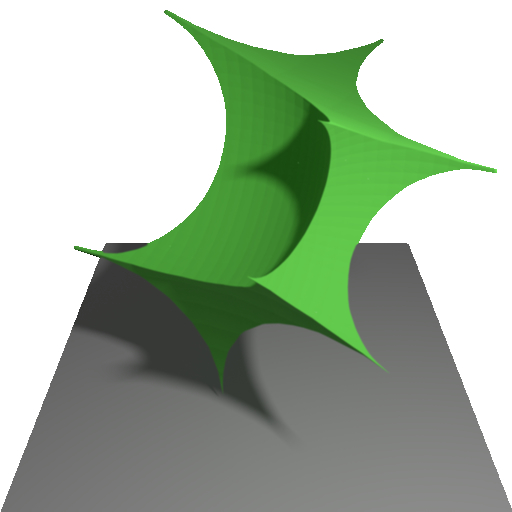
\includegraphics[height=1.2in, keepaspectratio]{./img/introduction/cube.jpg}
   \caption{Cubic sphairahedron.}
   \label{fig:cubeSphaira}
  \end{minipage}
  \hspace*{\fill}
 \begin{minipage}[t]{0.75\textwidth}
  \begin{minipage}[t]{0.25\textwidth}
   \centering
   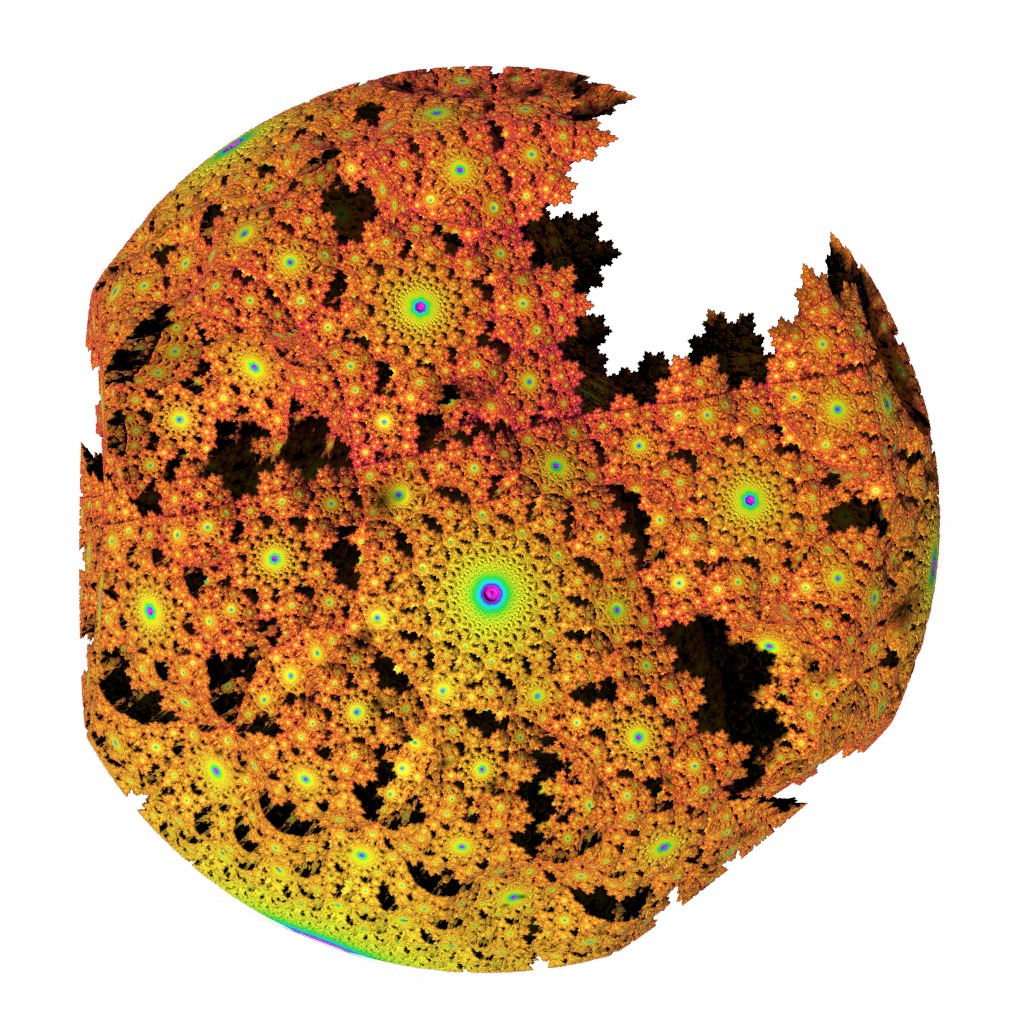
\includegraphics[height=1.2in,
   keepaspectratio]{./img/introduction/quasiSphere1.jpg}
   \subcaption{}
   \label{fig:quasi-sphere1}
  \end{minipage}
  \hspace*{\fill}
  \begin{minipage}[t]{0.25\textwidth}
   \centering
   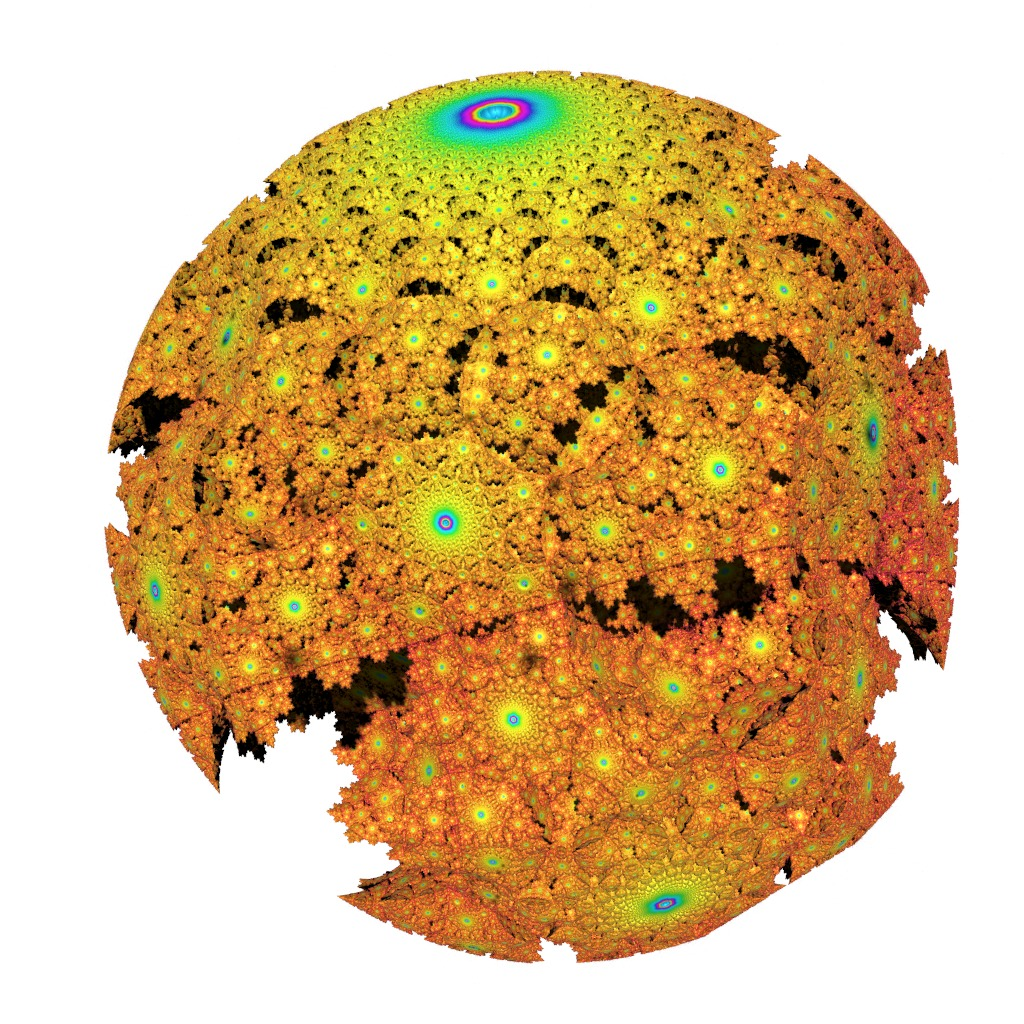
\includegraphics[height=1.2in,
   keepaspectratio]{./img/introduction/quasiSphere2.jpg}
   \subcaption{}
   \label{fig:quasi-sphere2}
  \end{minipage}
  \hspace*{\fill}
  \begin{minipage}[t]{0.25\textwidth}
   \centering
   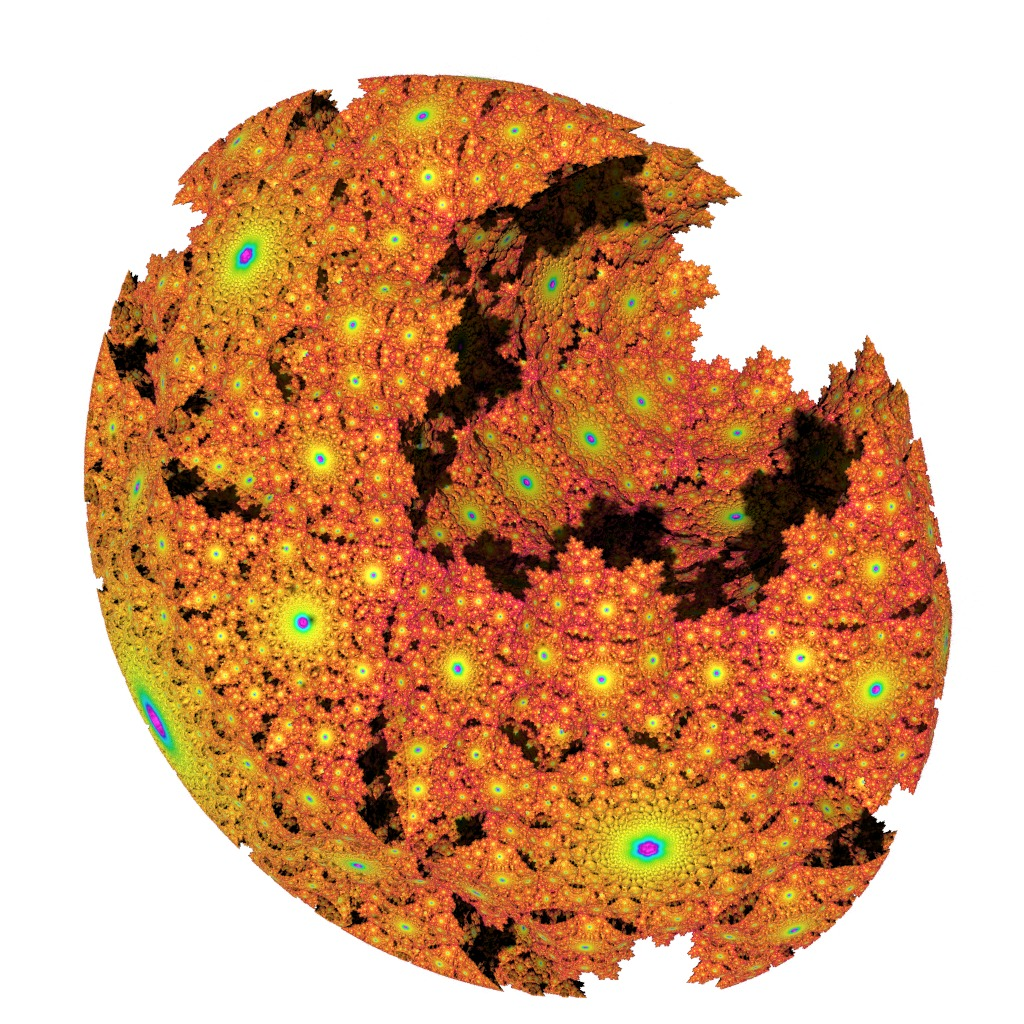
\includegraphics[height=1.2in,
   keepaspectratio]{./img/introduction/quasiSphere3.jpg}
   \subcaption{}
   \label{fig:quasi-sphereZoom}
  \end{minipage}
  \hspace*{\fill}
  \caption{Images of a quasi-sphere rendered in different viewpoints.}
  \label{fig:quasi-sphere}
 \end{minipage}
\end{figure}

\subsection{Background}

The main target of this paper is a visualization of four-dimensional
Kleinian groups, which is a discrete subgroup of the isometry group of
that four-hyperbolic space $H^4$. A four-dimensional Kleinian group $G$ acts
on $S^3$, the boundary of $H^4$ as a M\"obius transformation on
$S^3$. \par
There are few studies about a finitely generated M\"obius group on $S^3$,
and we start at a group arising from a sphairahedron introduced by Ahara
and Araki in 2003\cite{AharaAraki}.
Sphairahedron is a coined word combining two words 'sphaira' (a prefix
that means 'spherical') and 'hedron' (a suffix comes from 'polyhedron.')
It looks like a polyhedron, but each face is a part of a sphere. See
Figure \ref{fig:cubeSphaira}. It shows a cubic sphairahedron. The
polyhedral structure of the sphairahedron coincides with that of a usual cube.  In the sequel, if there is no confusion, we simply call it {\it a cube}.

We consider a group $G$ generated by the inversion of the six faces. An
inversion is an orientation reversing isometry. Thus we consider an
extended M\"obius transformation group; that is, we include both
orientation preserving and orientation reversion M\"obius transformations
and $\text{M\"ob}(S^3)$ denotes a group generated by all
sphere-inversions in $S^3$.

The group $G$ may give a tiling by sphairahedra in $S^3$. In some cases, the
boundary of the tiling space converges to a three-dimensional fractal
configuration. This boundary is the limit set of $G$. If it is
homeomorphic to a two-dimensional sphere $S^2$, we call it
\textit{quasi-sphere} and the group $G$ a quasi-fuchsian group. We show
an example of a quasi-sphere in Figure \ref{fig:quasi-sphere}.

Ahara and Araki studied graphics and mathematics about a sphairahedron
and a quasi-sphere in ICG 2002, that is, an international conference about
computer graphics.
The paper introduces mathematical background than the way of the rendering
graphics and it shows the simplest parameter space of cubic sphairahedra
and some rendered images of the limit set by POV-Ray.
After that, Ahara presented a paper written in Japanese\cite{AharaJa},
showing the varieties of sphairahedra and dimensions of parameter space.

In the graphical aspect, in 2012, Knighty developed a script to render
quasi-spheres in real-time under limited conditions\footnote{\url{http://www.fractalforums.com/ifs-iterated-function-systems/another-3d-kleinian/}}.
In 2014, J\'er\'emie Brunet published a book of
fractal paintings named ``L'art fractal''. One of his works in the book called
``Quasi-Quasi-Grail'' is based on Ahara and Araki fractal.

In 2017, a breakthrough came out.
Nakamura and Ahara developed an algorithm called
\textit{Iterated Inversion System (IIS)}\cite{bridges2016}\cite{bridges2017}.
They combine IIS and Sphere tracing\cite{sphereTracing},
 which is a kind of ray tracing,
and their technique allows us to render quasi-spheres dramatically fast.
IIS is a way to render CG related to a finitely generated group, whose
generators are symmetry transformations or inversions.
It determines a color on the screen pixel by pixel, thus, it get easy to parallelize and render an image fast.
Rendering quasi-sphere using IIS and sphere tracing is published in
Bridges\cite{bridges2018}, an international conference about mathematics
and arts.
This shows not only the way for CG but also an algorithm for mathematical art.

Note that there are many pictures of three-dimensional in this paper,
but it is hard to gaze their whole appearances only on paper. We can see a fractal renderer, more pictures, and more movies based on sphairahedra in
the web site\footnote{\url{https://sphairahedron.net}} of the first author.

This paper is organaized as follows.
In Section 1, we survey the history of sphairahedra and quasi-spheres.
In Section 2, we prepare the definitions of a sphairahedron and its tiling group.
In Section 3, we show some propositions about the parameter spaces of various kinds of sphairahedra.
In Section 4, we introduce some observations.

The authors thank their colleague Shoichi Fujita in their laboratory.
He provides valuable comments for them  to complete the calculations of
the parameter spaces of cake sphairahedra.


\section{Preparation}

\subsection{sphairahedron}

\begin{figure}[h!tbp]
  \begin{minipage}[t]{0.3\textwidth}
   \centering
   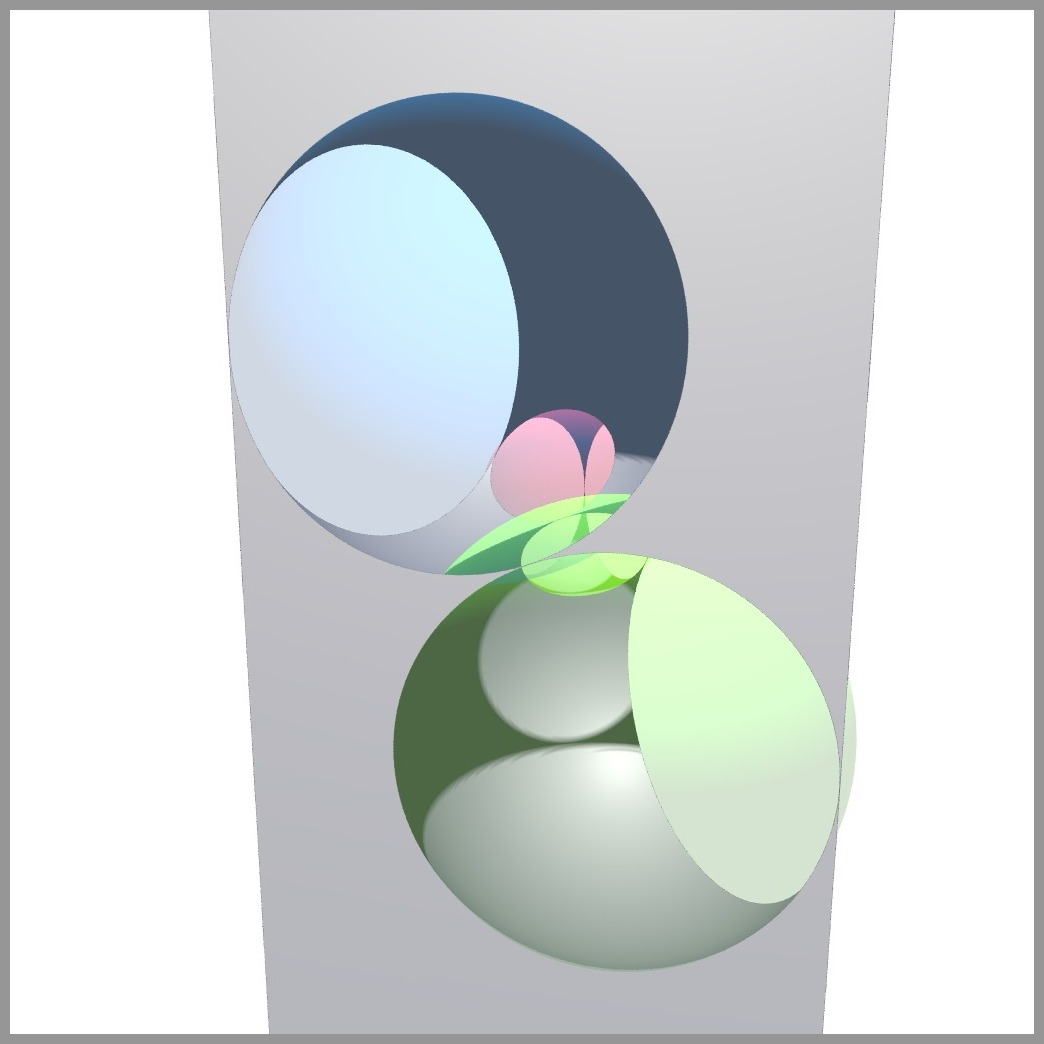
\includegraphics[width=1.2in, height=1.2in, keepaspectratio]
   {./img/sphairahedralPrism/sphairaAll.jpg}
   \subcaption{Complement $A$}
   \label{fig:sphairaPrismAll}
  \end{minipage}
  \hspace*{\fill}
  \begin{minipage}[t]{0.3\textwidth}
   \centering
   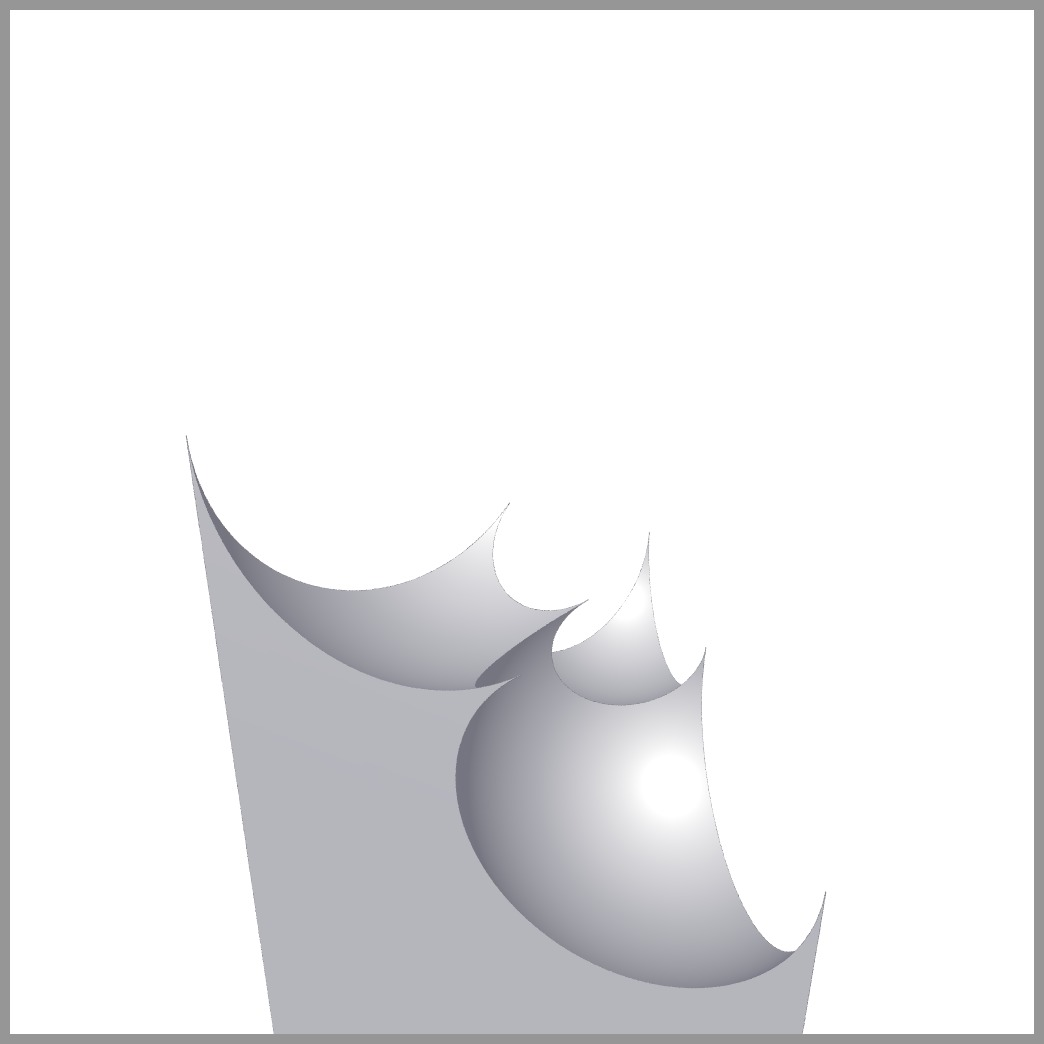
\includegraphics[width=1.2in, height=1.2in, keepaspectratio]
   {./img/sphairahedralPrism/sphairaHalf.jpg}
   \subcaption{Infinite}
   \label{fig:sphairaPrismHalf}
  \end{minipage}
  \hspace*{\fill}
  \begin{minipage}[t]{0.3\textwidth}
   \centering
   
\includegraphics[width=1.2in, height=1.2in,
   keepaspectratio]{./img/sphairahedralPrism/sphairahedron.jpg}
   \subcaption{Finite}
   \label{fig:sphairahedronFinite}
  \end{minipage}
  \hspace*{\fill}
  \caption{sphairahedron.}
  \label{fig:sphairahedron}
 \end{figure}

\begin{figure}[h!tbp]
 \begin{minipage}[t]{0.6\textwidth}
  \begin{minipage}[t]{0.3\textwidth}
   \centering
   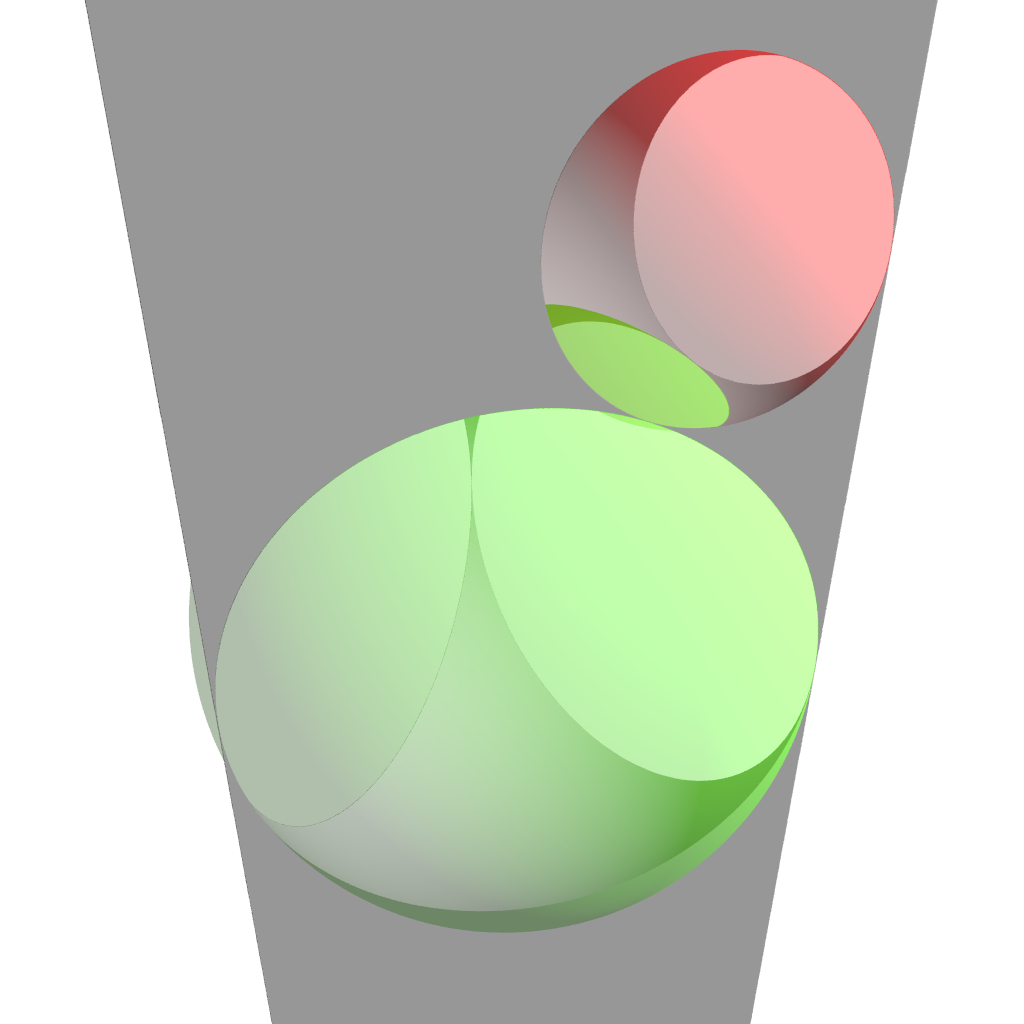
\includegraphics[width=1.2in, height=1.2in,
   keepaspectratio]{./img/sphairahedralPrism/semiSphairaAll.jpg}
   \subcaption{Complement $A$}
   \label{fig:semi-sphairaAll}
  \end{minipage}
  \hspace*{\fill}
  \begin{minipage}[t]{0.3\textwidth}
   \centering
   
\includegraphics[width=1.2in, height=1.2in,
   keepaspectratio]{./img/sphairahedralPrism/semiSphairaHalf.jpg}
   \subcaption{Infinite}
   \label{fig:semi-sphairaHalf}
  \end{minipage}
  \hspace*{\fill}
  \caption{Semi-sphairahedron.}
  \label{fig:semi-sphairahedron}
 \end{minipage}
 \begin{minipage}[t]{0.3\textwidth}
  \centering
 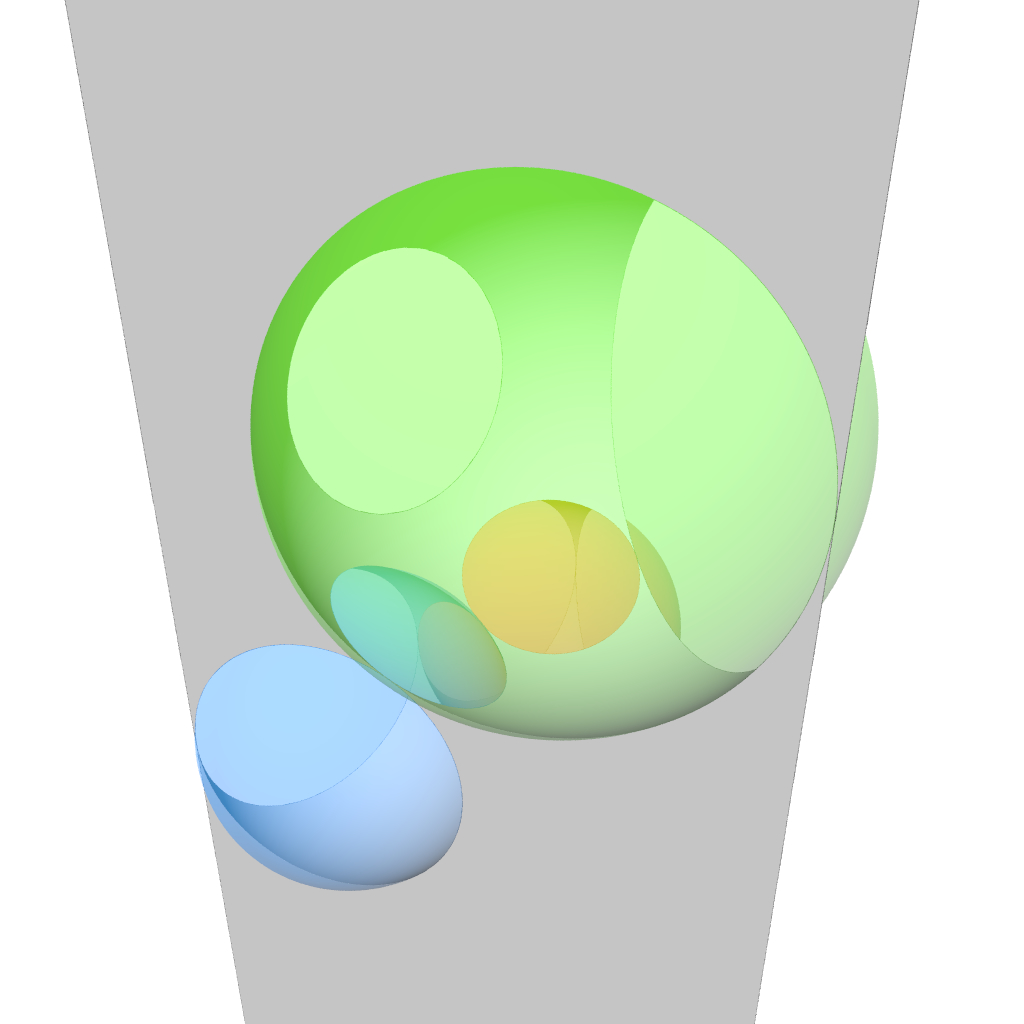
\includegraphics[width=1.2in, height=1.2in,
 keepaspectratio]{./img/sphairahedralPrism/hole.jpg}
 \caption{Sphairahedron with hole.}
  \label{fig:brokenHole}
 \end{minipage}
\end{figure}

We describe the definition of a sphairahedron used in \cite{bridges2018}.
\begin{definition}
Let $S^3 = R^3 \cup \{\infty\}$ be the three-dimensional sphere and let
$\overline{D_1},~\overline{D_2},\ldots,~\overline{D_p}$ be
three-dimensional closed balls or closed half-spaces in $S^3$.
We consider the complement $A$ of the union of these balls, that is,
$A = S^3 \setminus (\overline{D_1} \cup \overline{D_2} \cup ... \cup \overline{D_p})$.
If the following two conditions are satisfies, we call the component $T$ of $A$ a {\it sphairahedron.} \par
(a) \ $A$ consists of two connected components and all components are simply-connected.\par
(b) \ $T$ is a component of $A$, and for any $i$, a part of $O_i=\partial\overline{D_i}$ is a face of $T$.
\end{definition}
The image in Figure \ref{fig:sphairahedron}\subref{fig:sphairaPrismHalf}\subref{fig:sphairahedronFinite}
is an example of a sphairahedron.

By definition, a sphairahedron has faces, edges, and
vertexes. We define \emph{ideality} and \emph{rationality} of a sphairahedron.

\begin{definition}
(1)\ Let $T$ be a sphairahedron.  For each vertex, if all edges passing through the vertex are tangential to each other, we call it an \emph{ideal} sphairahedron.\par
(2)\ Let $T$ be a sphairahedron.  For each edge, if the dihedral angle at the edge is rational (that is, the angle equals to $\pi/n$, where $n$ is a natural number,) we call it an \emph{rational} sphairahedron.
\end{definition}

In the sequel, we mainly consider an ideal rational sphairahedron.
When one of the vertices is the infinite-point $\infty$ of $S^3$,
we call the sphairahedron \textit{infinite sphairahedron}.
One example is shown in Figure
\ref{fig:sphairahedron}\subref{fig:sphairaPrismHalf}.
Here, we consider a triangular prism with infinitely length and we hollow
out it by three balls, and select one of the connected components as a  sphairahedron.  A face adjacent to the infinite vertex is a plane, the boundary of the half space.  Thus the neighborhood of the infinite vertex is a prism.

When the closure of a sphairahedron does not contain the infinite point,
we call it \textit{finite sphairahedron}.
See Figure\ref{fig:sphairahedron}\subref{fig:sphairahedronFinite}.

%--------
% We hollow out the $S^3$ with six balls: we remove three half-spaces
% (three balls with infinite radius,) from $S^3$ and obtain the prism of
% infinite length, and we scoop out the prism by the remaining
% three-colored transparent balls as in Figure
% \ref{fig:sphairahedron}\subref{fig:sphairaPrismAll}.
% $A$ is composed of two parts, and each of the components is simply connected.
% Since it has six faces, and these faces are arranged as those of faces of
% a cube, it is called a cubic sphairahedron.
% Especially, the sphairahedron showned in Figure
% \ref{fig:sphairahedron}\subref{fig:sphairaPrismHalf}
% is also called an \textit{infinite type sphairahedron},
% because one of the vertexes of the sphairahedron is at the infinity.
% Similarly, the shape hollowed out by six finite balls in Figure
% \ref{fig:sphairahedron}\subref{fig:sphairahedronFinite} is called a
% \textit{finite type sphairahedron}.
%----------

Moreover, we can loosen the definition of an ideal rational sphairahedron,
that is, we allow the case $A$ has simply connected three or more components.

\begin{definition}
Let $\overline{D_1}, \overline{D_2},\ldots, \overline{D_p}$ be ball or
half-space in $S^3$.  Let $A$ be the complement of the unions of
$\overline{D_i}$'s.  If the following three conditions are satisfies, we call the subset $T$ {\it a semi-sphairahedron.}\par
(a) \ $A$ has more than two connected components and all
components are simply connected. \par
(b) \ $T$ is a component or the union of two (or more) components, and the closure $\text{Cl}(T)$ is connected. \par
(c) \ For any $i$, a subset of $O_i=\partial \overline{D_i}$ is a face of $T$.
\end{definition}
Figure \ref{fig:semi-sphairahedron}\subref{fig:semi-sphairaAll} shows an
example of a ideal rational semi-sphairahedron.  We can get this shape by scooping a
triangle prism out by two balls.  Complement $A$ consists of three
connected components. Lower two of them are tetrahedra, and the upper
one is a pentahedron.  If we set $T$ to be the unions of lower two components,
then $T$ is a semi-sphairahedron and we can regard it as a sphairahedron with a singular point.  See Figure \ref{fig:semi-sphairahedron}\subref{fig:semi-sphairaHalf}.


Remark that Ahara and Araki \cite{AharaAraki},
and Kageyama \cite{kageyama} did not deal with semi-sphairahedra and their rendering images.

Other than semi-sphairahedra, we have much more 'sphairahedron-like
shapes' in the ideal and rational situation.  See Figure \ref{fig:brokenHole}. In this
figure, we see a hole indicated by an arrow at one of the faces.  This shape does not generate a
sphairahedron, but we can apply the tiling method in the below section,
and we have a (non-simply-connected) limit set.  We have not classified
these figures mathematically yet, but possibly it occurs some
interesting geometry problems from here.


\subsection{Limit set}\label{constructFractal}

\begin{figure}[h!tbp]
 \begin{minipage}[t]{0.18\textwidth}
  \centering
  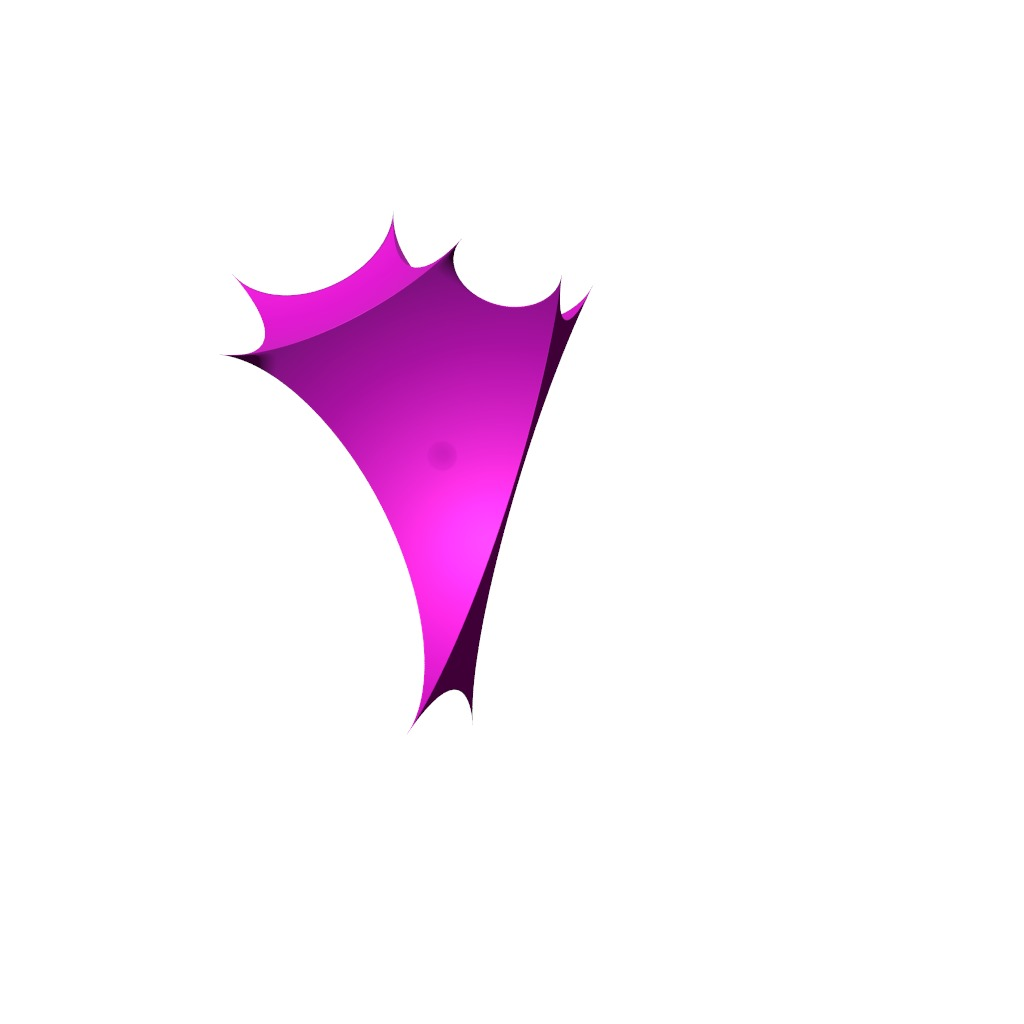
\includegraphics[width=1in, height=1in, keepaspectratio]{./img/constructFractal/finiteProcess/step1.jpg}
  \subcaption{Step 1}
  \label{fig:sphaira-step1}
 \end{minipage}
 \hspace*{\fill}
 \begin{minipage}[t]{0.18\textwidth}
  \centering
  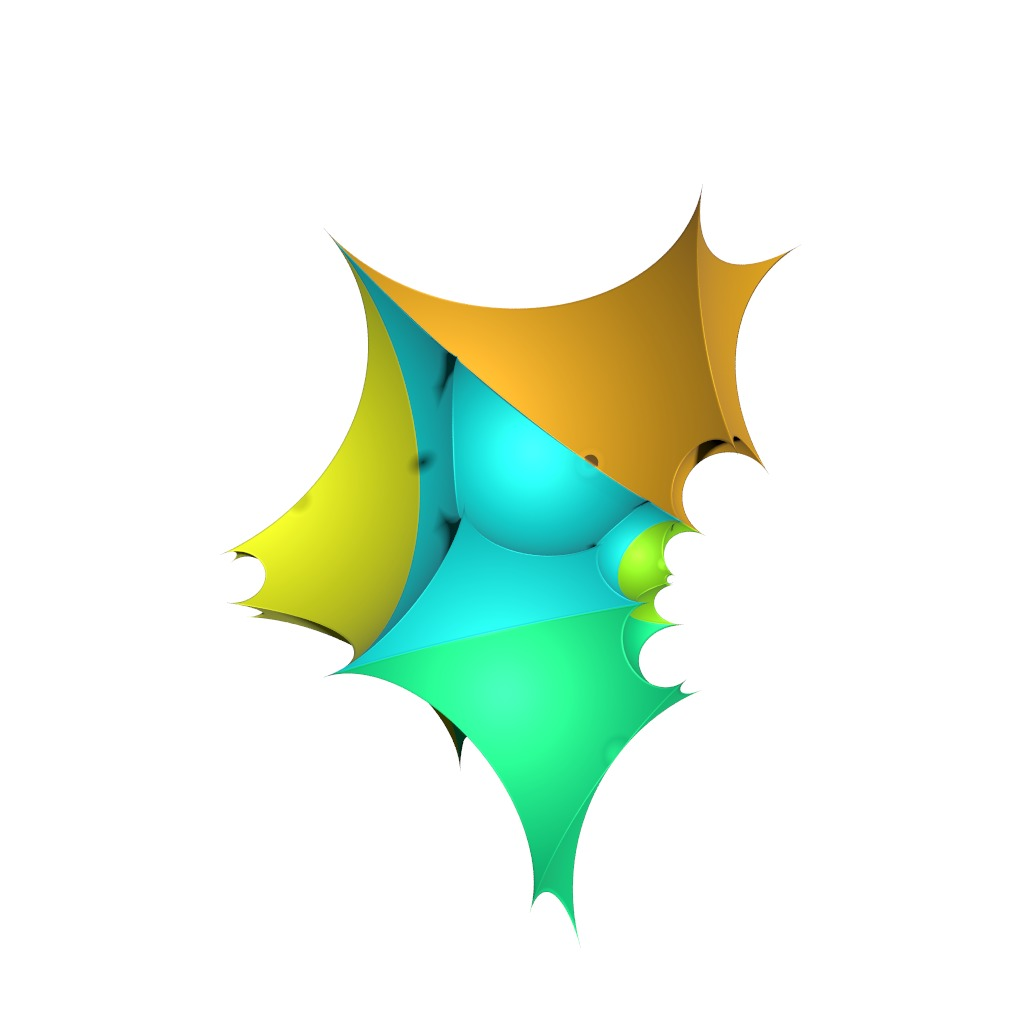
\includegraphics[width=1in, height=1in, keepaspectratio]{./img/constructFractal/finiteProcess/step2.jpg}
  \subcaption{Step 2}
  \label{fig:sphaira-step2}
 \end{minipage}
 \hspace*{\fill}
 \begin{minipage}[t]{0.18\textwidth}
  \centering
  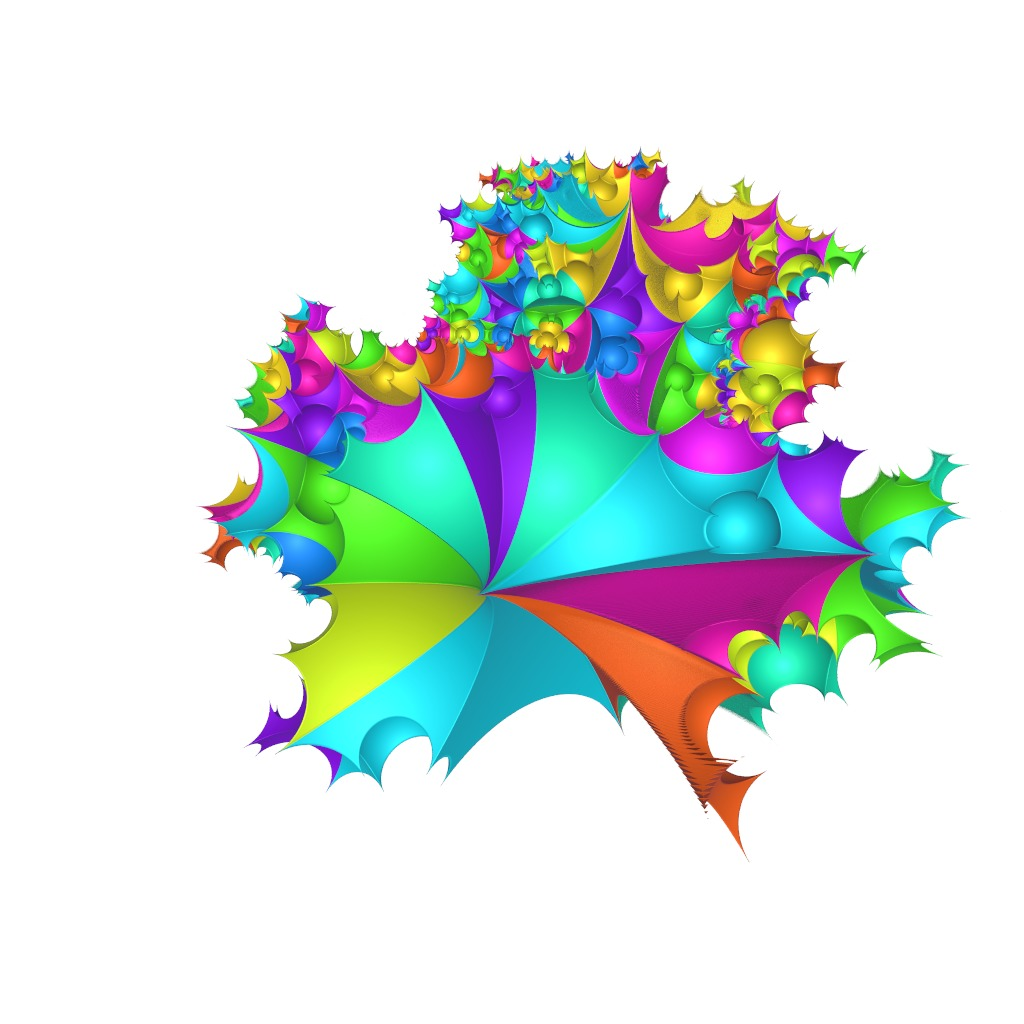
\includegraphics[width=1in, height=1in, keepaspectratio]{./img/constructFractal/finiteProcess/step5.jpg}
  \subcaption{Step 5}
  \label{fig:sphaira-step5}
 \end{minipage}
 \hspace*{\fill}
 \begin{minipage}[t]{0.18\textwidth}
  \centering
  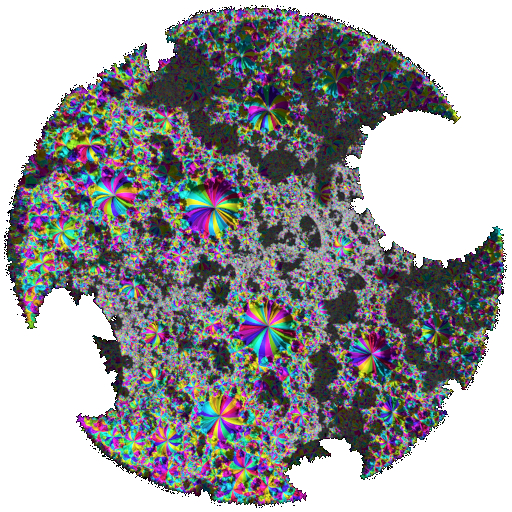
\includegraphics[width=1in, height=1in, keepaspectratio]{./img/constructFractal/finiteProcess/step10.jpg}
  \subcaption{Step 10}
  \label{fig:sphaira-step10}
 \end{minipage}
 \hspace*{\fill}
 \begin{minipage}[t]{0.18\textwidth}
  \centering
  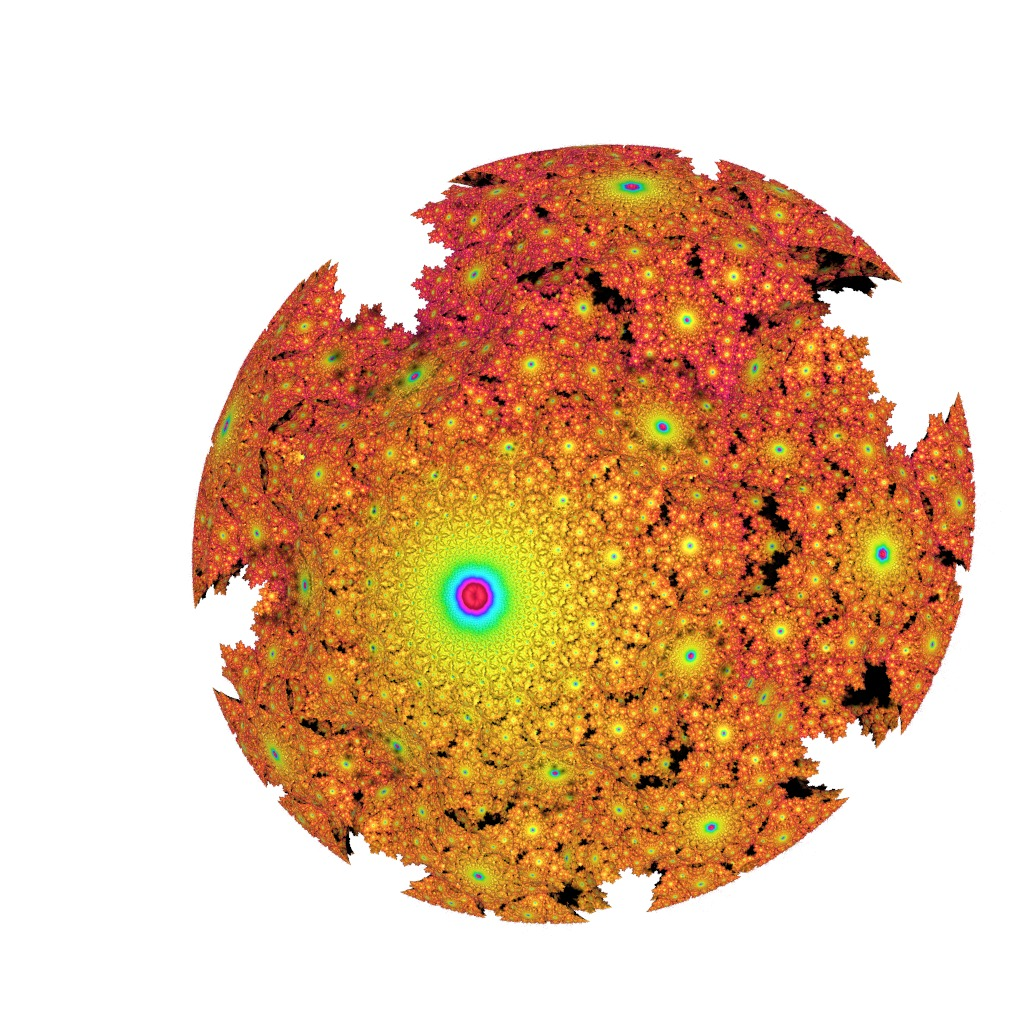
\includegraphics[width=1in, height=1in, keepaspectratio]{./img/constructFractal/finiteProcess/final.jpg}
  \subcaption{Final image}
  \label{fig:sphaira-final}
 \end{minipage}
 \hspace*{\fill}
 \caption{Tiling of a finite cubic}
 \label{fig:sphairahedronTile}
\end{figure}

Let $T$ be a sphairahedron.  Let $\overline{D_i}$ ($i = 1,2,\ldots, p$) be the closed ball of $T$ and $O_i$ be the boundary sphere of $\overline{D_i}$.  Suppose that a map $\varphi_i:S^3 \to S^3$ is the inversion map of $O_i$.  $\varphi_i$ is an orientation-reversing M\"obius map on $S^3$ and let the {\it tiling group} $G=G(T)$ be a group generated by all $\varphi_i$'s.  That is,
\[
 G = G(T) := \langle\varphi_1, \varphi_2, \ldots , \varphi_p  \rangle < \text{Mob}(S^3)
\]

For a subgroup $G$ of
$\text{Mob}(S^3)$, let the {\it discontinuity set} $\Omega(G)$ be
\[
\Omega(G) = \left\{ x \in S^3 \left| \hspace{1mm}
\begin{minipage}{8cm}
the point $x$ possesses a neighborhood $U(x)$
such that the intersection $U(x) \cap gU(x)$ is empty for all but finite
elements $g\in G$
\end{minipage}
 \right. \right\}.
\]
The complement $\Lambda(G) := S^3 \backslash \Omega(G)$ is called the
{\it limit set} of the group $G$. $G$ is a (4 dimensional) {\it Kleinian group} if $\Omega(G)$ is
not empty\footnote{Usually we consider a Kleinian group as a properly discontinuous subset of the {\it orientation preserving} M\"obius transformation group $\text{Mob}_+(S^3)$, however we weaken the condition of orientation preserving.}. The limit set $\Lambda(G)$ consists either of 0 or 1 or 2 or
infinitely many points. Here we consider only the case that $\Lambda(G)$
is infinite and two-dimensional.
A Kleinian group $G$ is called a
{\it 3-Kleinian group} if $\Lambda(G)$ is a round sphere. This means that $G$ can be reduced into the Kleinian group $\text{Mob}(S^2)$ in the usual sense.
A Kleinian group $G$ is called a
{\it quasi-fuchsian group} if $\Lambda(G)$ is homeomorphic to a closed sphere,
and there exists a homeomorphism $f:S^3 \rightarrow S^3$ which conjugates
$G$ to a 3-Kleinian group. If $G$ is a quasi-fuchsian group, the limit set
$\Lambda(G)$ may be a fractal sphere, that is, a sphere embedded in $S^3$ with
 fractal structure.

%球面体をタイリングすることができる。(ポアンカレの多面体定理)
Let $L$ be the tiling generated by a tile $T$ and a transform group $G$, that is, the piece set of $L$ consists of $g(T)$ for all $g\in G$.  We represent $L$ by the pair $(T,G)$.  The rationality condition guarantees the local consistency of tiling satisfies because of Poincare's polyhedron theorem.

%実際に、群$G$の長さが短い要素から考えていくと、その和集合はローカルには球体と同相な図形の$S^3$へのはめ込み(局所的な埋め込み)になる。
Let $|L|_k$ be the interior of the union of tiles $g(\text{Cl}(T))$ such that the word length of $g\in G$ is less than $k+1$.  That is,
\[
|L|_k := \text{Int}\left( \bigcup _{(\text{length of }g)<k+1} g(\text{Cl}(T)) \right).
\]
At least for a small $k$, $|L|_k$ is homeomorphic to a open 3-ball $B^3$.  For a large $k$ there are no guarantee to be a 3-ball, though if we consider the universal covering $\widetilde{|L|_k}$ of the union of tiles, $\widetilde{|L|_k}$ is a ball for any $k$.  There is a natural immersion $i_k:\widetilde{|L|_k}\to|L|_k\subset S^3$.  The tiling $L=(T,G)$ is {\it embedded} in $S^3$ if the immersion $i_k$ is an embedding for any $k$.  Whether a given tiling $L$ can be embedded in $S^3$ depends on the shape of the fundamental sphairahedron $T$ and it is not trivial to show this.  We call the limit $\displaystyle\bigcup_k|L|_k$ {\it the total tiling space}.

Using sphairahedron.net\cite{sphairahedron_net}, we can observe rendered images of $|L|_k$.  See Figure \ref{fig:sphairahedronTile}.   In Figure
\ref{fig:sphairahedronTile}\subref{fig:sphaira-step1} we see the fundamental sphairahedron with six faces.  $|L|_1, |L|_5, |L|_{10}$ is shown in Figure
\ref{fig:sphairahedronTile}\subref{fig:sphaira-step2}\subref{fig:sphaira-step5}\subref{fig:sphaira-step10}.
In these figure, adjacent tiles have different colors.  In Figure
\ref{fig:sphairahedronTile}\subref{fig:sphaira-step10}, outside tiles
are so small and we see the union in gray color.  These figures suggest
us that $|L|_k$'s are embedded in $S^3$.  Figure
\ref{fig:sphairahedronTile}\subref{fig:sphaira-final} shows a rendering
image for a large enough $k$.  In this figure we use another algorithm(,
detemining a color by $k$ on the hue circle) to render the image and we
success to color the shape properly. 

We show another example of $|L|_k$ in Figure \ref{fig:sphairahedralPrismTile}.  In this example the fundamental tile is an infinite sphairahedron.  The resulting shape in Figure \ref{fig:sphairahedralPrismTile}\subref{fig:sphairaPrismFinal} looks like a terrain of scenic beauty.

Observation using simulator repeatedly is beneficial to find conjecture.
Here we present a conjecture after observation of the simulations by
sphairahedron.net\cite{sphairahedron_net}.

\begin{conjecture}
If $T$ is an ideal rational sphairahedron, and $G$ is the tiling group of $T$, then the tiling $L=(T,G)$ is embedded in $S^3$.
\end{conjecture}

Here we see the limit set of the group $G$.  In fact it is well-known that the limit set is the closure of the accumulation point set of an orbit.  Using this characteristic, we have the following.

\begin{lemma}
If the tiling $L=(T,G)$ is embedded in $S^3$, then we have
\[
\Lambda(G) =\partial\left(\bigcup_k |L|_k\right)
\]
\end{lemma}

\begin{figure}[h!tbp]
 \begin{minipage}[t]{0.18\textwidth}
  \centering
  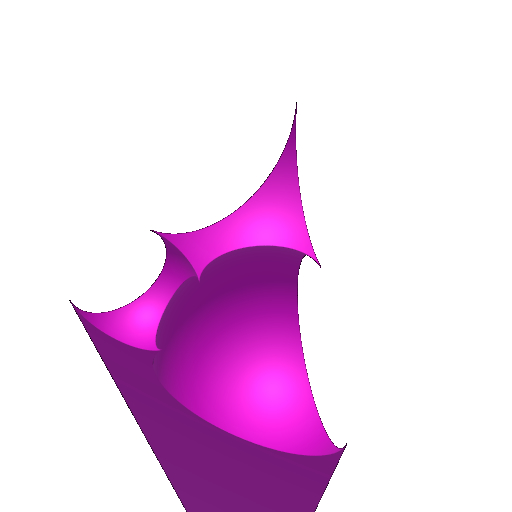
\includegraphics[height=1.1in, keepaspectratio]{./img/constructFractal/terrainProcess/step1.jpg}
  \subcaption{Step 1}
  \label{fig:terrainStep1}
 \end{minipage}
 \hspace*{\fill}
 \begin{minipage}[t]{0.18\textwidth}
  \centering
  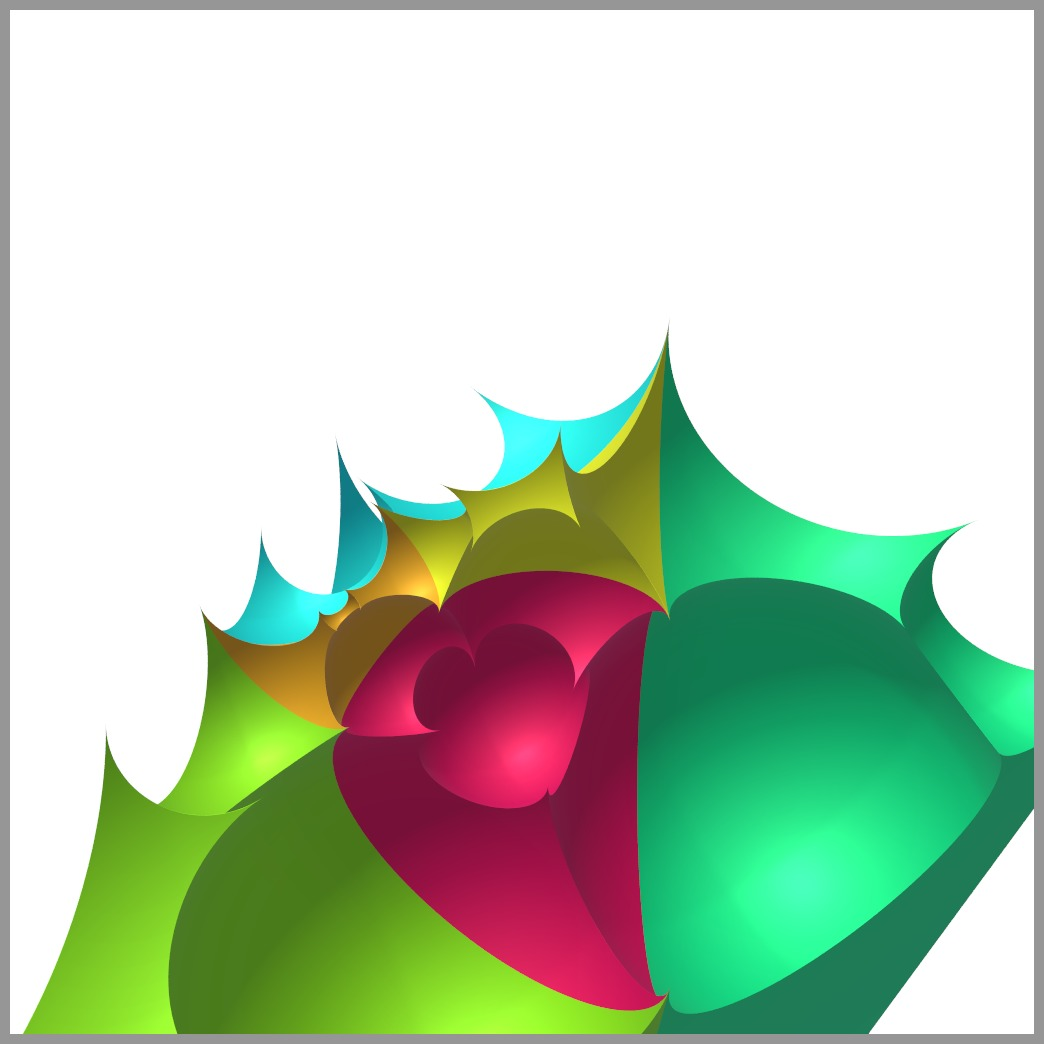
\includegraphics[height=1.1in, keepaspectratio]{./img/constructFractal/terrainProcess/step2.jpg}
  \subcaption{Step 2}
  \label{fig:terrainStep2}
 \end{minipage}
 \hspace*{\fill}
 \begin{minipage}[t]{0.18\textwidth}
  \centering
  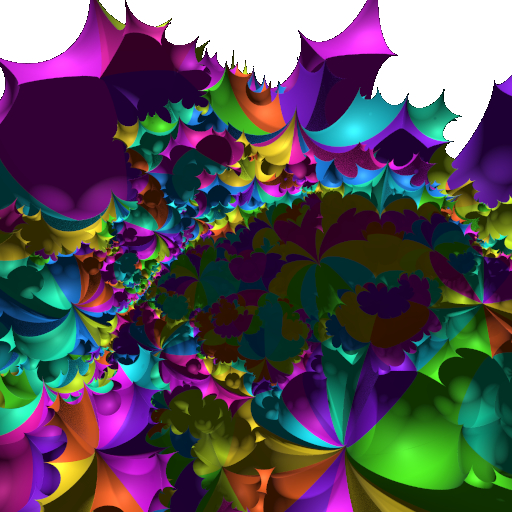
\includegraphics[height=1.1in, keepaspectratio]{./img/constructFractal/terrainProcess/step5.jpg}
  \subcaption{Step 5}
  \label{fig:terrainStep5}
 \end{minipage}
 \hspace*{\fill}
 \begin{minipage}[t]{0.18\textwidth}
  \centering
  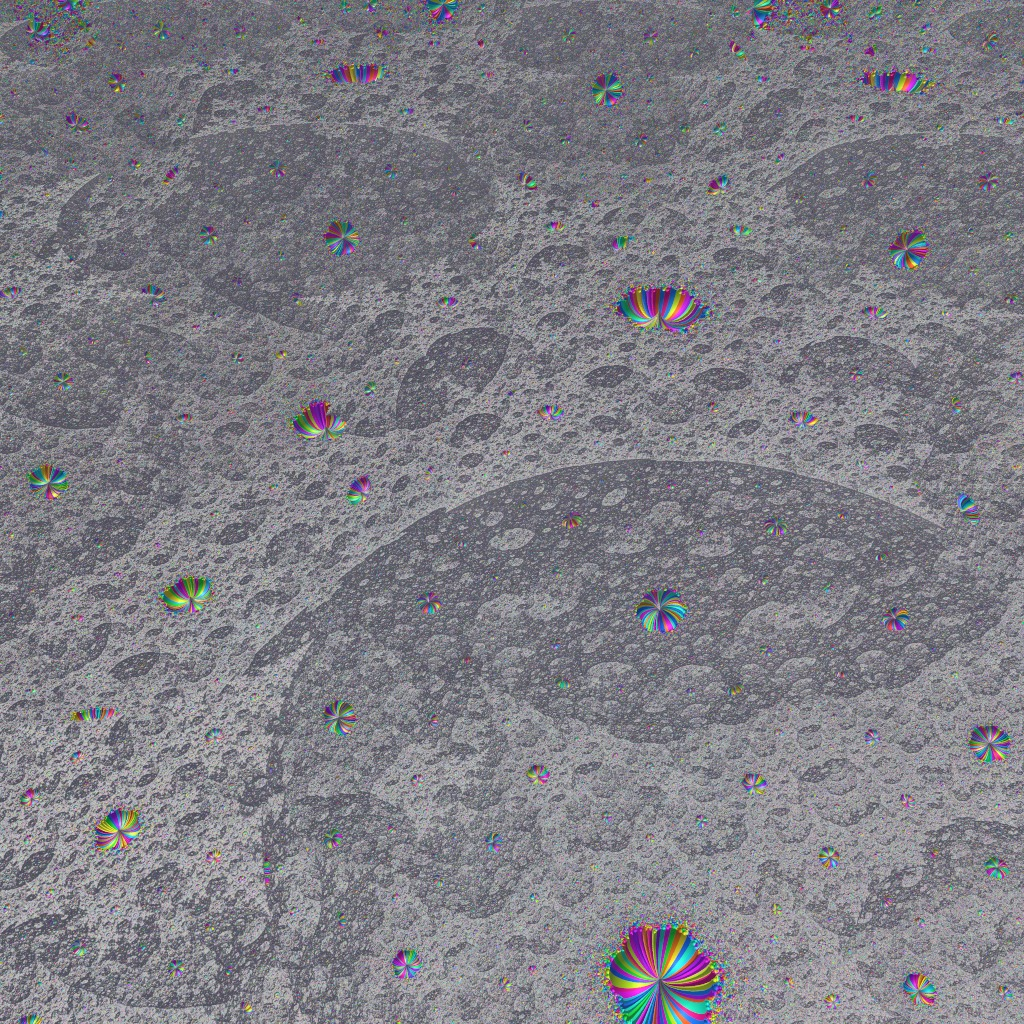
\includegraphics[height=1.1in, keepaspectratio]{./img/constructFractal/terrainProcess/step20.jpg}
  \subcaption{Step 20}
  \label{fig:terrainStep20}
 \end{minipage}
 \hspace*{\fill}
 \begin{minipage}[t]{0.18\textwidth}
  \centering
  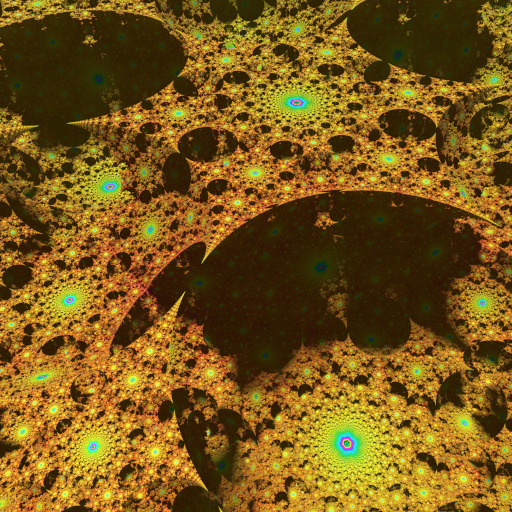
\includegraphics[height=1.1in, keepaspectratio]{./img/constructFractal/terrainProcess/final.jpg}
  \subcaption{Final image}
  \label{fig:sphairaPrismFinal}
 \end{minipage}
 \caption{Tiling of a infinite cubic sphairahedron.}
 \label{fig:sphairahedralPrismTile}
\end{figure}

\begin{figure}[h!tbp]
  \centering
 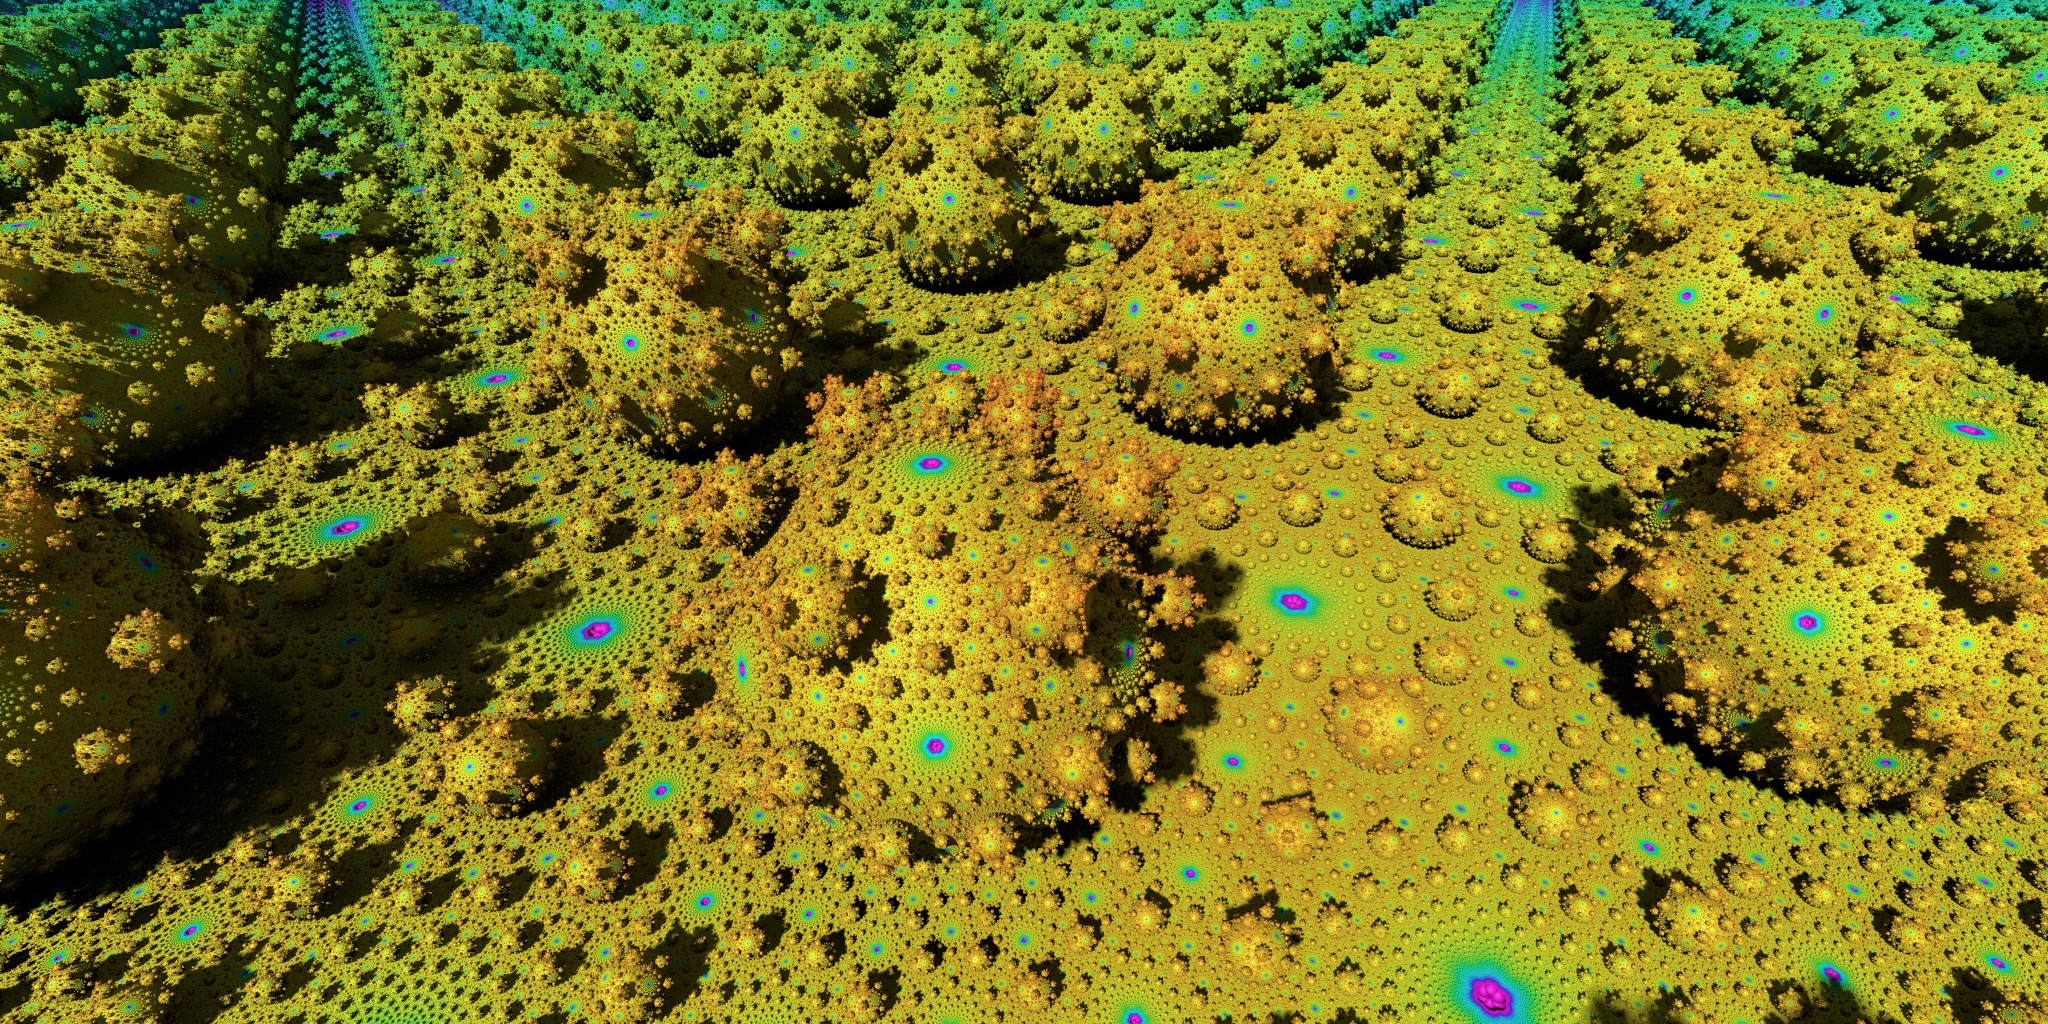
\includegraphics[width=3in,
 keepaspectratio]{./img/constructFractal/semi-terrain.jpg}
 \caption{Plane and infinite number of balls touching to the ground.}
  \label{fig:semiSphairaSpheres}
\end{figure}

%semi-sphairahedronについてはここで書く。
In the same way as above, a semi-sphairahedron
can be tiled by the inversions of its faces.
Though the fundamental tile may be not connected and each $|L|_k$ is not connected nor the group is not quasi-fuchsian, the closure $\text{Closure}(|L|_k)$ is connected.
See an example in Figure \ref{fig:semiSphairaSpheres}.  Here we see an plane and infinite number of balls touching to the ground and to each other.  We call this shape {\it snowball fractal.}  Such shape can occur lower side of the plane, that is, we see only one plane but there are infinite number of spherical pitfalls underground.

%%対称性については、「数学的知見」のところで扱う。
%Also, an infinite sphairahedron can be tiled, as presented in Figure
%\ref{fig:sphairahedralPrismTile}.
%The pattern converges to fractal terrain owing to reflections over side
%faces of the sphairahedron, as shown in Figure
%\ref{fig:sphairahedralPrismTile}\subref{fig:terrainStep1}.
%In the fractal terrain, we can find symmetry easily.
%For example, we can see hexagram-like terrain patterns in Figure
%\ref{fig:sphairahedralPrismTile}\subref{fig:sphairaPrismFinal}.
%These patterns are originated from the dihedral angles of the side faces of
%$\pi / 3$.
%
%
%In the images of fractals within this paper, each tile of the
%sphairahedra is colored according to the
%number of inversions.
%We use the color wheel to determine their color,
%and the tile's color varies in order of red, yellow, green, and blue.
%In Figure \ref{fig:sphairahedronTile}\subref{fig:sphaira-step1} $\sim$ \subref{fig:sphaira-step10} and
%Figure \ref{fig:sphairahedralPrismTile}\subref{fig:terrainStep1} $\sim$ \subref{fig:terrainStep20},
%we refer color wheel with large steps to visualize each tile clearly.
%On the other hand, in the other images, we refer the wheel with smaller
%steps, and we find lots of tiles with many inversions in the blue
%parts of the fractal.

%Up to this point, we showed tiling patterns without gaps between the tiles and
%intersections of the tiles.
%However, not every sphairahedra can generate such proper tiling patterns.
%To obtain them, we have to consider two mathematical properties
%of the original sphairahedron. That is, the sphairahedron should be
%rational and ideal.
%In the following sections, we will introduce these properties and
%compute parameter space for the rational ideal sphairahedron.

\section{Parameter Spaces of Rational Ideal Sphairahedra}

\subsection{Classification of Sphairahedra}

%We are interested in finding examples of quasi-fuchsian sub-group of
%M\"ob$_{+}(S^3)$, the group of orientation preserving M\"obius
%transformation on $S^3 = R^3 \bigcup \{\infty\}$.
%For a subgroup $G$ of
%Mob$_+(S^3)$, let the discontinuity set $\Omega(G)$ be
%$$
%\Omega(G) = \left\{ x \in S^3 \left| \hspace{1mm}
%\begin{minipage}{8cm}
%the point x possesses a neighborhood $(x)$
%such that the intersection $U(x) \cap gU(x)$ is empty for all but finite
%elements $g\in G$
%\end{minipage}
% \right. \right\}.
%$$
%The complement $\Lambda(G) := S^3 \backslash \Omega(G)$ is called the
%limit set of the group $G$. $G$ is a Kleinian group if $\Omega(G)$ is
%not empty. The limit set $\Lambda(G)$ consists either of 0 or 1 or 2 or
%infinitely many points. Here we consider only the case that $\Lambda(G)$
%is infinite and two-dimensional. A Kleinian group $G$ is a fuchsian
%group if $\Lambda(G)$ is a closed round sphere. $G$ is called a
%quasi-fuchsian group is $\Lambda(G)$ is homeomorphic to a closed sphere,
%and there exists a homeomorphism $f:S^3 \rightarrow S^3$ which conjugates
%$G$ to a fuchsian group. If $G$ is a quasi-fuchsian group, the limit set
%$\Lambda(G)$ may be a fractal sphere, that is, a sphere in $S^3$ with
%fractal structure.

%In two dimensional case, that is, $G$ is a subgroup of M\"ob$_+(S^2)$
%(or equivalently M\"ob$_+(H^3)$, we have many examples of quasi-fuchsian
%groups.) One of the important examples is a kissing Schottky group.
%Let $O_1^+, O_2^+, O_1^-, O_2^-$ be circles in $S^2$ such that
%$O_1^{\pm}$ are tangential to $O_2^{\pm}$. Let $f_i$ be a M\"obius
%transformation which maps the exterior of $O_i^+$ onto the interior of
%$O_i^{-}$ for $i = 1, 2$ and let a group $G$ be generated by $f_1, f_2$.
%(Remark that $\Lambda$ is homeomorphic to a circle if a set of the
%tangent points is equivalent under the action of $G$. See p.157 of
%\cite{indra}.)
%If the four circles are disjoint to each
%other, we call $G$ a Schottky group and $\Lambda(G)$ is an infinite set
%but is not homeomorphic to a circle. We may consider the case that
%$O_1^{\pm}$ intersects to $O_2^{\pm}$ by $\pi/n$ for a natural number
%$n$. In this case, we also have a circle-wise limit set $\Lambda(G)$.
%See p361 of \cite{indra}.

%The Coxeter-like group is another example. Consider 4 (or more) circles in
%$S^2$ (we call them 'initial circles.') Let $\tilde G$ be a group generated
%by the inversions of these initial circles. Here we assume that any two
%initial circles are disjoint or tangential or intersecting  by angle
%$\pi/n$ for $n \in N$. Then a subgroup $G$, which is defined by a set of
%all even-length-elements of $\tilde G$, is well-defined.
%
%In this article, we consider an extension of kissing Schottky groups and
%Coxeter-like groups to M\"ob($S^3$). In order to do that, we have to
%obtain a set of initial spheres (instead of 'initial circles') with some
%conditions. the following new problem of Euclidean geometry is
%one of the good approaches.

%\begin{problem}
% Let $S^3 = R^3 \bigcup {\infty}$. Find a polyhedron in $S^3$ satisfying
% the following conditions.
% \begin{description}
%  \item[Condition 1:] Each face of a polyhedron is a sphere in $S^3$.
%  \item[Condition 2 (rationality):] For each edge, the face-angle equals $\pi/n$
%             for a natural number $n$.
%  \item[Condition 3 (ideality):] For each vertex, edges with the vertex are
%             mutually tangent at the vertex.
% \end{description}
%\end{problem}

%In the following sections, we derive rational ideal sphairahedron.

In this section we consider ideal rational sphairahedra of various types.
In order to classify such sphairahedra, we need three steps.  In the first step, we classify the polyhedral structure of a sphairahedron.  See Figure \ref{fig:tetrahedronFinite} for a tetraheron.  This example is a sphairahedron of tetrahedron type, this means that the polyhedral structure is same as that of a tetrahedron as in Figure \ref{fig:tetrahedronFaces}.
In the second step, we classify combinations of dihedral angles of edges.  In tetrahedron case, there are three combinations as seen in Figure \ref{fig:tetrahedronCombinations}.  Here a number $n$ at each edge means that the dihedral angle at the edge is $\pi / n$.
In the third step, we calculate the parameter space of the shape of sphairahedra.  Here we assume that two sphairahedra $T_1, T_2$ are equivalent if there exists a (orientation preserving/reversing) M\"obius transformation $f$ on $S^3$ such that $f(T_1) = T_2$.  In the tetrahedron case, the parameter space consists of only one point.

%阿原荒木の仕事
Ahara and Araki \cite{AharaAraki} determine all of combinations of dihedral angles of the cubic sphairahedra and they show one of the parameter space without a proof.
%阿原の仕事
Ahara \cite{AharaJa} determines all of polyhedral structures of sphairahedra with 5 or 6 faces.  He also shows the number of combinations of dihedral angles for each structure without a proof.
Ahara and Araki \cite{AharaAraki2} determines all of the parameter spaces for the cube case with a proof.  This paper was quoted in other papers, however it is an unpublished preprint.
%影山さんの仕事(の関連部分)の紹介
Kageyama \cite{kageyama} quotes the result of \cite{AharaAraki2} in his master thesis in order to prove
the existence of other variations of sphairahedra.
%この論文での守備範囲の紹介
In this chapter, we show the parameter spaces of sphairahedra with 5 or
6 faces, including current results.
The proof repeats similar discussions as those in \cite{AharaAraki2},
and we enumerate the results in Appendix.


%Usually, a polyhedron has planar faces. But easily, we can consider an
%extension of a polyhedron such that the faces are a part of a
%sphere. (Hence each edge is an arc.) If we have such polyhedron with
%the above conditions, we consider spheres of the faces as initial
%spheres. Easily we can consider a Coxeter-like group generated by the
%inversions of them.

%In this article, we first consider a polyhedron with the same cellular
%structure as that of a cube. (Hence the number of the initial spheres is
%6.) And we have the following result.

%\begin{theorem}\label{main}
% If a polyhedron with the above conditions is of cubic (that is,
% the one skeleton of the polyhedron is the same as that of a cube), then
% there are seven combinations of face-angles. For each combination of
% face-angles, a set of conformagl equivalent classes of polyhedra is two
% dimensional.
%\end{theorem}

%Once we have a polyhedron $P$ with the above conditions, we may consider
%a Coxeter-like subgroup $G=G(P)$ of M\"ob$_+(S^3)$. Through proving this
%theorem, we obtain that for each combination of dihedral angles, there is a
%polyhedron such that the limit set $\Lambda(G)$ is a round sphere. So,
%other polyhedra give us quasi-fuchsian groups. So we get a family of
%a quasi-fuchsian group with two parameters. At the same time, we have a
%family of fractal spheres with two parameters.

% This paper is organized as follows. In the section 2 we will show the
% above theorem. In the section 4 we consider other type
% of polyhedra and show a similar theorems.

\subsubsection{General lemmas}
We prepare some lemmas to execute classifications.

\begin{lemma}\label{lemma:sum}
Suppose that there are $k$ edges with a vertex. Then the sum of
 dihedral angles of these three edges is $(k-2)\pi$.  If $k=3$ then the combination of dihedral angles is
one of $\left( \frac{\pi}{3}, \frac{\pi}{3}, \frac{\pi}{3}\right)$, $\left( \frac{\pi}{2}, \frac{\pi}{4}, \frac{\pi}{4}\right)$, and $\left( \frac{\pi}{2}, \frac{\pi}{3}, \frac{\pi}{6}\right)$.
If $k=4$ then the combination of dihedral angles is
$\left( \frac{\pi}{2}, \frac{\pi}{2}, \frac{\pi}{2}, \frac{\pi}{2}\right)$. The case $k>4$ cannot happen.
\end{lemma}

\begin{proof}
 Let $\phi$ be a M\"obius transformation such that it maps the vertex to
 the infinite-point. Then all of edges with the vertex are mapped to
 parallel lines, and they form a prism. If we consider a
 regular section of a prism, then the internal angles of the section
 are equal to dihedral angles, and the sum of them is $(k-1)\pi$.  This
 completes the proof.  We easily have all combinations of dihedral angles.
\end{proof}

Next, we prepare some lemmas to calculate the parameter space of sphairahedra. First, we recall simple conditions to be equivalent of two sphairahedra.  This lemma is clear because it is well known that these transformations are M\"obius transformations.

\begin{lemma} \label{lemma:equivalentOfSH}
Suppose that two sphairahedra $T_1, T_2$ satisfy that $T_2=\varphi(T_1)$, where $\varphi$ is a parallel translation or a rotation or a dilation or a plane-symmetry or a composite of these transformations.  Then $T_1, T_2$ are equivalent.
\end{lemma}

\subsubsection{Situation 1}
Next, we consider a infinite sphairahedron without loss of generality.  In fact, $T$ is a spahairahedron, and  let $P$ be one of vertices and let $\varphi$ be a M\"obius transformation satisfying $\varphi(P)=\infty$.  Thus, $T'=\varphi(T)$ has the infinite vertex, and we may assume that one of the vertices is the infinite point.

Beacause of the ideality of a sphairahedron, all edges with the infinite vertex are parallel straight lines.  Using rotations, we assume that these edges are parallel to the $z$-axis.  It follows that the faces with the finite vertex are perpendicular with $xy$-plane.

Let $A$ be one of finite vertices next to the infinite vertex, that is, there exists an edge $e_{12}$ that connects $A$ and $\infty$.  After applying translations, we assume that the edge $e_{12}$ lies on the $z$-axis.  In fact we suppose the followings as Situation 1:
\begin{align*}
A &= (0,0,z_A),\\
\overline{D_1}  &= \{ (x,y,z) \mid 0 \le y \} \cup \{\infty\} ,\\
\overline{D_2}  &= \{ (x,y,z) \mid 0 \le x\sin\theta_{12} - y\cos\theta_{12} \}\cup \{\infty\} ,\\
\overline{D_3}  &= \{ (x-x_3)^2+(y-y_3)^2+(z-z_3)^2 \le r_3^2 \}, \\
O_i & = \partial(\overline{D_i}) \qquad(i=1,2,3,)
\end{align*}
where the vertex $A$ is on the $z$-axis, $\overline{D_i}$'s are closed balls, $\theta_{12}$ is the dihedral angle of $S_1$ and $S_2$,  $(x_3, y_3, z_3)$ is the center of the face $O_3$, and $r_3$ is the radius of $O_3$.  We assume that $A$ is the intersection of $O_1, O_2, O_3$.  We have the following equation including dihedral angles and  $x_3, y_3, z_3, r_3$.

\begin{lemma} \label{lemma:CenterOfSphere}
In Situation (1), suppose $\theta_{13}$ is the dihedral angle of $S_1$ and $S_3$   We have the followings.\par
(1) $z_3=z_A$,\par
(2) $r_3^2 = x_3^2+y_3^2$, \par
(3) $x_3\cos\theta_{13} - y_3\sin\theta_{13}=0$.\par
Conversely, if $\overline{D_3}$ satisfies (1), (2) then the edges $O_1 \cap O_2$, $O_1 \cap O_3$, $O_2 \cap O_3$ are tangent to each other at $A$.  If $\overline{D_3}$ satisfies (1), (2), and (3) then the dihedral angle of $S_1$ and $S_3$ is $\theta_{13}$.
\end{lemma}

\begin{figure}[h!tbp]
 \centering
 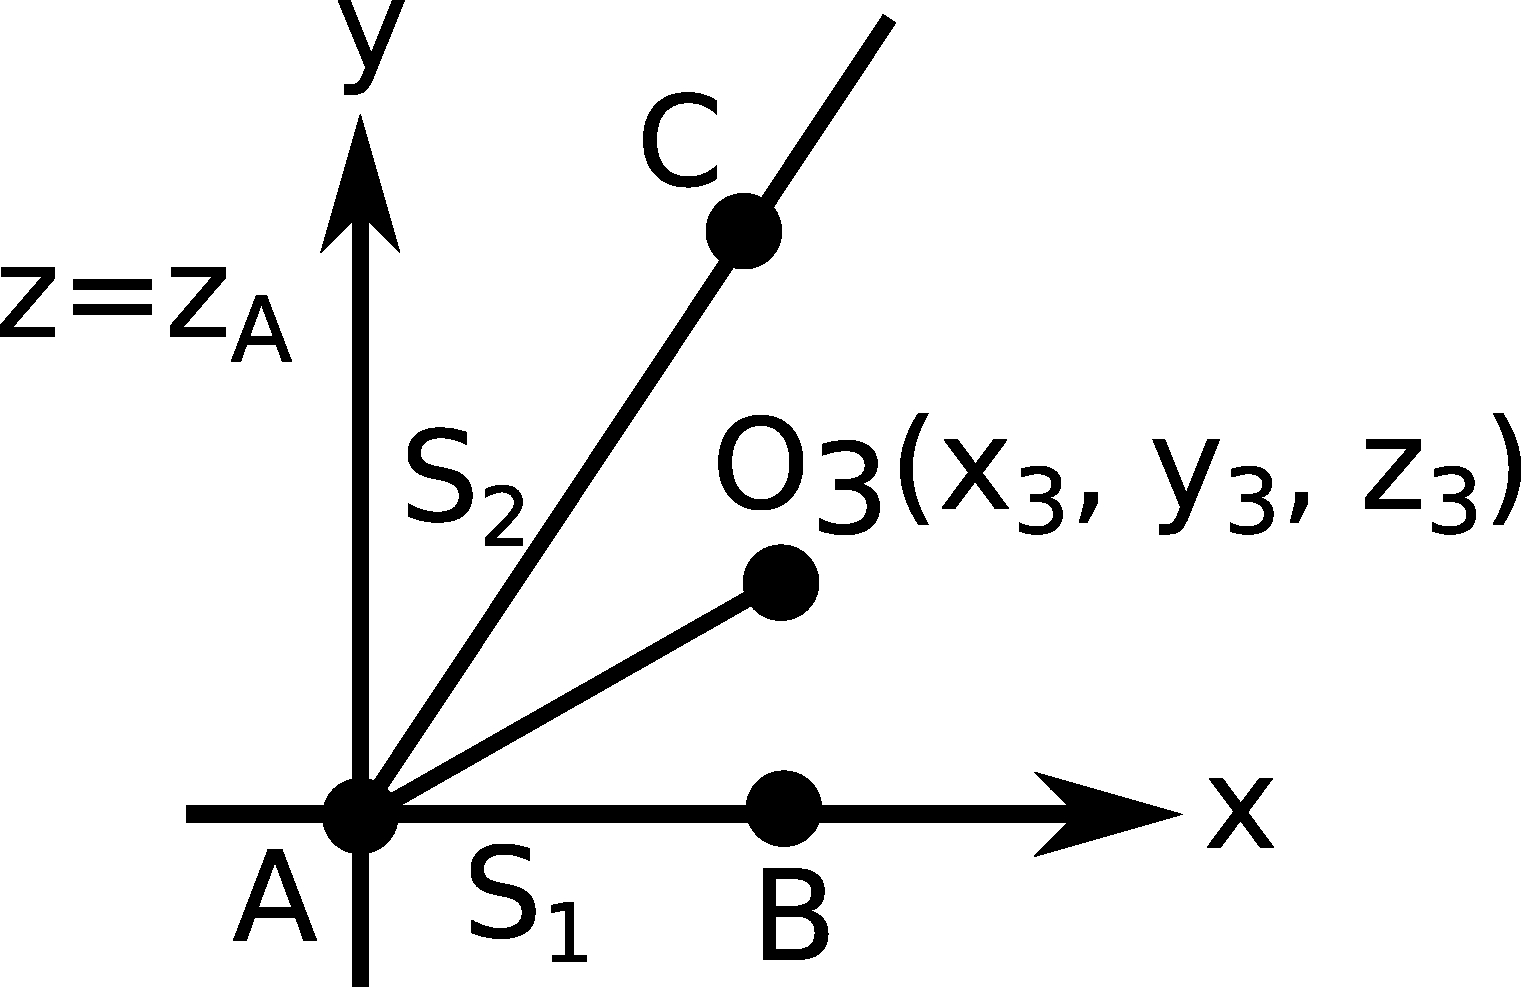
\includegraphics[width=1.5in, height=1.5in,
 keepaspectratio]{./img/HexahedraWithSphericalFaces/sectionAtVertex.jpg}
 \caption{Section at $a=z_A$.}
 \label{fig:sectionAtVertex}
 \hspace*{\fill}
\end{figure}

\begin{proof}
Figure \ref{fig:sectionAtVertex} shows the section at $z=z_A$.  Let points $B, C$ be as seen in Figure \ref{fig:sectionAtVertex}.  By definition, $\angle BAC=\theta_{12}$.  Let $e_{13}$ be the intersection of the plane $S_1$ and the sphere $S_3$.  Then $e_{13}$ is a circle on the $xz$ plane and it is tangent to the $z$-axis at $A$ because of the ideality.  Therefore the height $z_3$ of the center $O_3$ must be the same as that $A$, and we have $z_3 = z_A$.\par
The center $O_3$ of $S_3$ lies on the section $z=z_A$ and the sphere $S_3$ includes the point $A$, hence $r_3^2 = x_3^2+y_3^2$.
Because the dihedral angle of the plane $S_1$ and the sphere $S_3$ is $\theta_{13}$,  the angle $\angle BAO_3$ is $\frac{\pi}{2}-\theta_{13}$.  $x_3\cos\theta_{13} - y_3\sin\theta_{13}=0$ follows immediately.
\end{proof}

\begin{remark}
If the vertex $A$ is of degree $3$, the same observation works on the dihedral angle $\theta_{23}$ of $S_2$ and $S_3$.  In fact $\angle O_3AC=\frac{\pi}{2}-\theta_{23}$ in Figure \ref{fig:sectionAtVertex}.  Thus we have $\theta_{12}+\theta_{23}+\theta_{13}=\pi$ and this equation is compatible with Lemma \ref{lemma:sum}.
\end{remark}

After considering more general situations, we obtain the following corollary.

\begin{corollary}\label{cor:tangencyOfEdge}
Let each $O_1, O_2, O_3$ be a sphere or a plane.  Let $e_{ij}=O_i\cap O_j$ be a non-empty edge and let $\theta_{ij}$ be the dihedral angle of $O_i$ and $O_j$. Suppose that $\theta_{12}+\theta_{23}+\theta_{13}=\pi$ and that $e_{12}$ and $e_{13}$ are  tangent to each other at a point $P$.  Then $e_{12}$, $e_{13}$ and $e_{23}$ are tangent at $P$ and $O_1\cap O_2\cap O_3=\{ P \}$.
\end{corollary}
%%%%%%%%%%%%%%%%%%%%%%%%%%%%

\subsubsection{Situation 2}
We need another situation as Situation 2:
\begin{align*}
\overline{D_1}  &= \{ (x,y,z) \mid y \le 0 \} \cup \{\infty\} ,\\
A &= (0,0,0)\\
\overline{D_2}  &= \{ (x,y,z) \mid (x-x_2)^2+(y-y_2)^2+(z-z_2)^2<r_2^2\}\\
B &= (w,0,z_B)\\
\overline{D_3}  &= \{ (x,y,z) \mid (x-x_3)^2+(y-y_3)^2+(z-z_3)^2<r_3^2\}\\
O_i & = \partial(\overline{D_i}) \qquad(i=1,2,3,)
\end{align*}
where
\begin{align*}
z_2&=0,\  r_2^2=x_2^2+y_2^2,\  x_2\cos\theta_{12}-y_2\sin\theta_{12}=0,\ 0 < y_2\\
z_3&=z_B,\  r_3^2=(x_3-w)^2+y_3^2,\  (x_3-w)\cos\theta_{13}+y_2\sin\theta_{13}=0,\ 0<y_3,
\end{align*}
and $w (0<w), \theta_{12} (0<\theta_{12}\le \frac{\pi}{2}), \theta_{13}  (0<\theta_{13}\le \frac{\pi}{2})$ are constants.  From Lemma \ref{lemma:CenterOfSphere}, the dihedral angle of $O_1$ and $O_2$ (resp. $O_1$ and $O_3$) is $\theta_{12}$ (resp. $\theta_{13}$.)


The following lemma gives a condition that two edges $O_1\cap O_2$ and $O_1\cap O_3$ are tangent to each other.

\begin{lemma} \label{lemma:twoCirclesChain}
We consider a section by $y=0$ in Situation 2 as seen in Figure \ref{fig:twoCirclesChain}.  The left side circle is $O_1\cap O_2$ and the right side circle is $O_1\cap O_3$.  The left circle is tangent to $x=0$ at $A$ and it has the center $C$.  The right circle is tangent to $x=w$ at $B$ and it has the center $D$. \par
If and only if two circles are tangent to each other, the following equation holds.
\[
r_2\sin\theta_{12}+r_3\sin\theta_{13}=\dfrac{w^2+z^2}{2w}
\]
\end{lemma}

\begin{figure}[h!tbp]
  \centering
  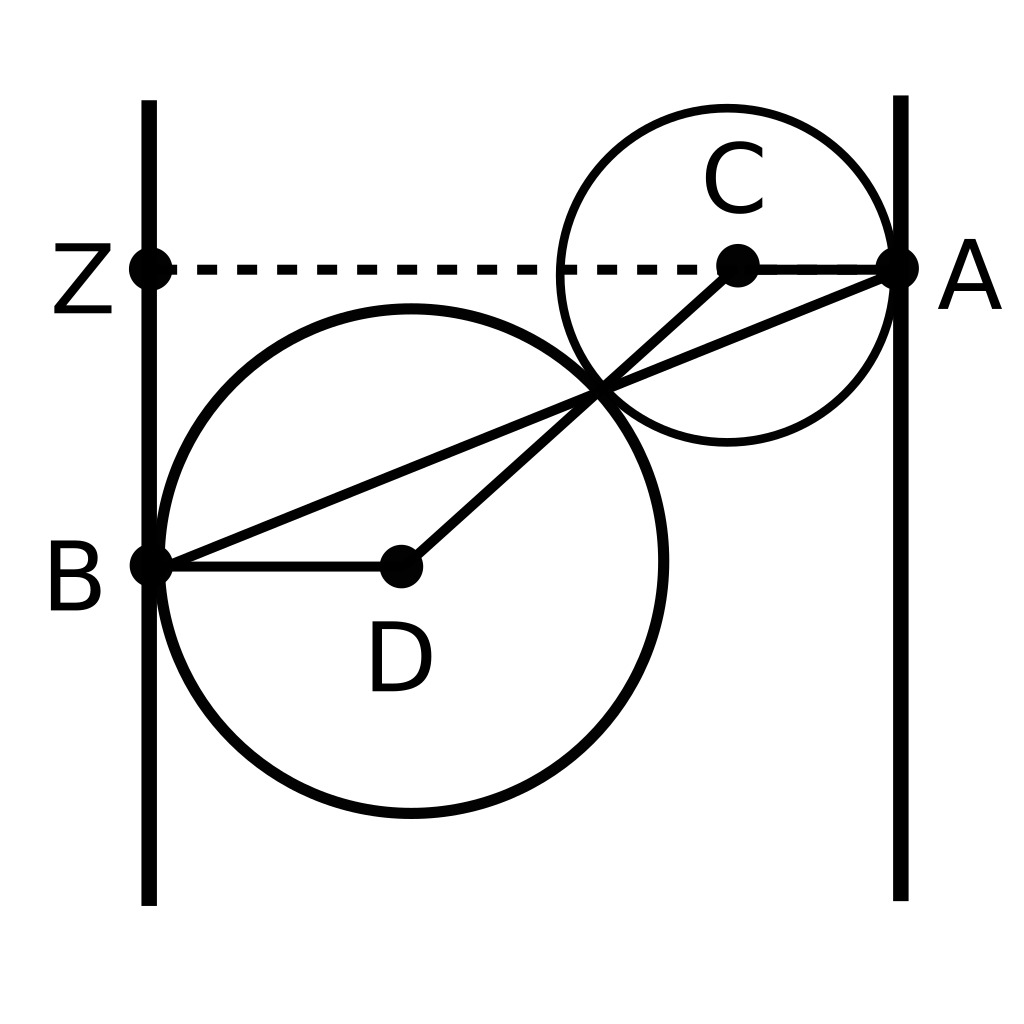
\includegraphics[width=1.5in, height=1.5in,
  keepaspectratio]{./img/HexahedraWithSphericalFaces/twoCirclesSlice.jpg}
 \caption{Two tangent circles.}
 \label{fig:twoCirclesChain}
\end{figure}

\begin{proof}
The proof is very elementary, and we show it by simplified description.  Let $\theta$ be $\angle CAB$.  We have
\[
\dfrac{w}{\sin\theta}  = \sqrt{w^2+z^2}
 = (r_2\sin\theta_{12}+r_3\sin\theta_{13})\cdot(2\sin\theta ).
\]
The equation $r_2\sin\theta_{12}+r_3\sin\theta_{13}=\dfrac{w^2+z^2}{2w}$ follows immediately from these two equations.  It is easy to show the converse proposition.
\end{proof}

\begin{lemma} \label{lemma:twoCirclesChainAngle}
Suppose that the condition of the above lemma is satisfies.\par
(1)\ The dihedral angle $\theta_{23}$ of $O_2$ and $O_3$ is equal to $\pi - \theta_{12} - \theta_{13}$ \par
(2)\ The intersection edge $e_{23}$ of $O_2$ and $O_3$ is tangent to the two circle in Figure \ref{fig:twoCirclesChain} at the tangent point in the same figure.
\end{lemma}

\begin{proof}
From the cosine law, we have
\[
\cos (\pi - \theta_{23}) = \dfrac{r_2^2+r_3^2 - \{(x_2-x_3)^2+(y_2-y_3)^2+(z_2-z_3)^2\}}{2 r_2r_3}.
\]
The coordinates of the centers of $O_2$ and $O_3$ are given by
$(x_2,y_2,z_2)=(r_2\sin\theta_{12},  r_2\cos\theta_{12}, 0)$, and
$(x_3,y_3,z_3)=(w - r_3\sin\theta_{13},  r_3\cos\theta_{13}, z_B)$.
Using $z_B^2+w^2 = 2w(r_2\sin\theta_{12}+r_3\sin\theta_{13})$, we have
\[
(x_2-x_3)^2+(y_2-y_3)^2+(z_2-z_3)^2=r_2^2+r_3^2-2r_2r_3\cos(\theta_{12}+\theta_{13}).
\]
Thus $\cos (\pi - \theta_{23})=\cos(\theta_{12}+\theta_{13})$ and $\theta_{23} = \pi - \theta_{12} - \theta_{13}$.\par
(2)\ Let $P$ be the tangent point in Figure \ref{fig:twoCirclesChain}.  Applying the result of (1) to Corollary \ref{cor:tangencyOfEdge}, we show that $e_{23}$ is tangent to $O_1\cap O_2=e_{12}$ and $O_1\cap O_3=e_{13}$ at $P$.  The proof completes.

\end{proof}

\subsection{Tetrahedron}\label{section:tetrahedron}

\begin{figure}[h!tbp]
  \begin{minipage}[t]{0.5\textwidth}
   \centering
   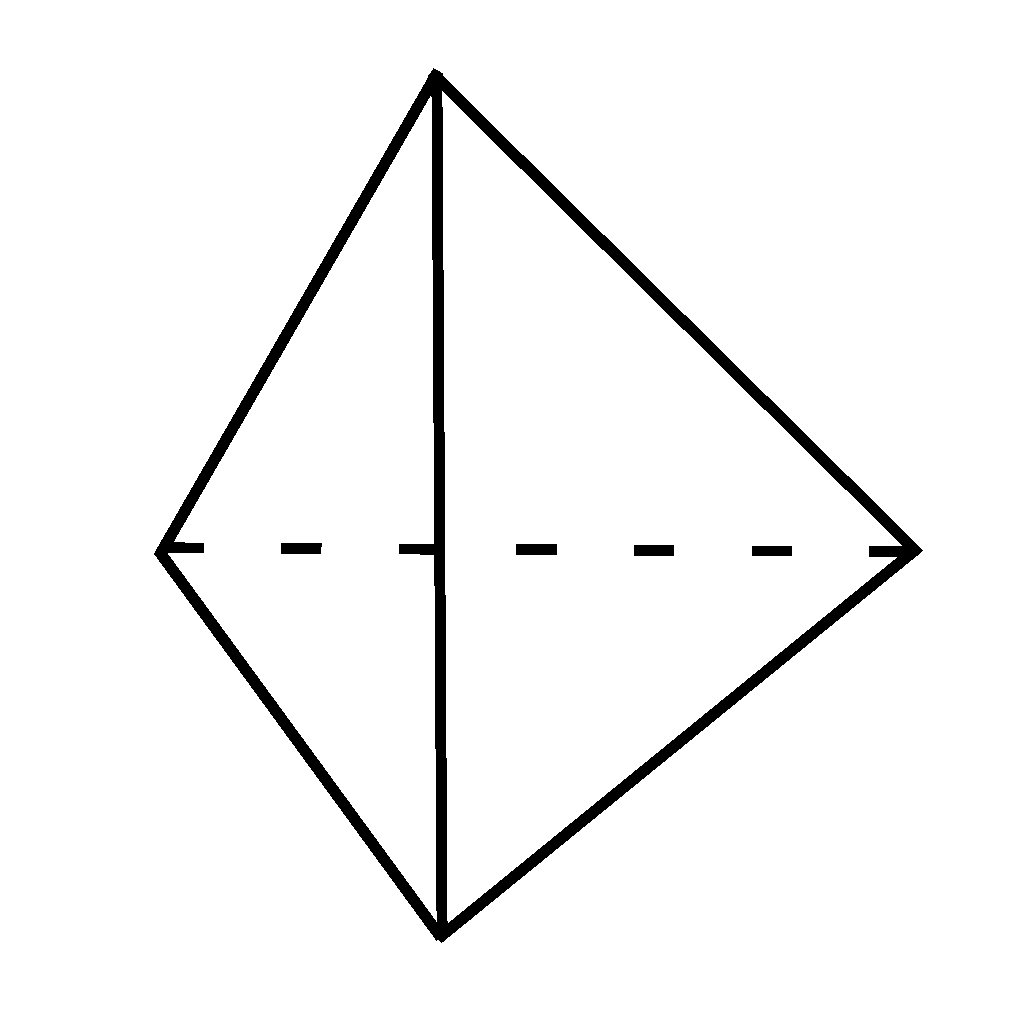
\includegraphics[width=1in, keepaspectratio]{./img/HexahedraWithSphericalFaces/tetrahedron/tetrahedron.jpg}
   \caption{Tetrahedron.}
   \label{fig:tetrahedron}
  \end{minipage}
 \hspace*{\fill}
  \begin{minipage}[t]{0.5\textwidth}
   \centering
   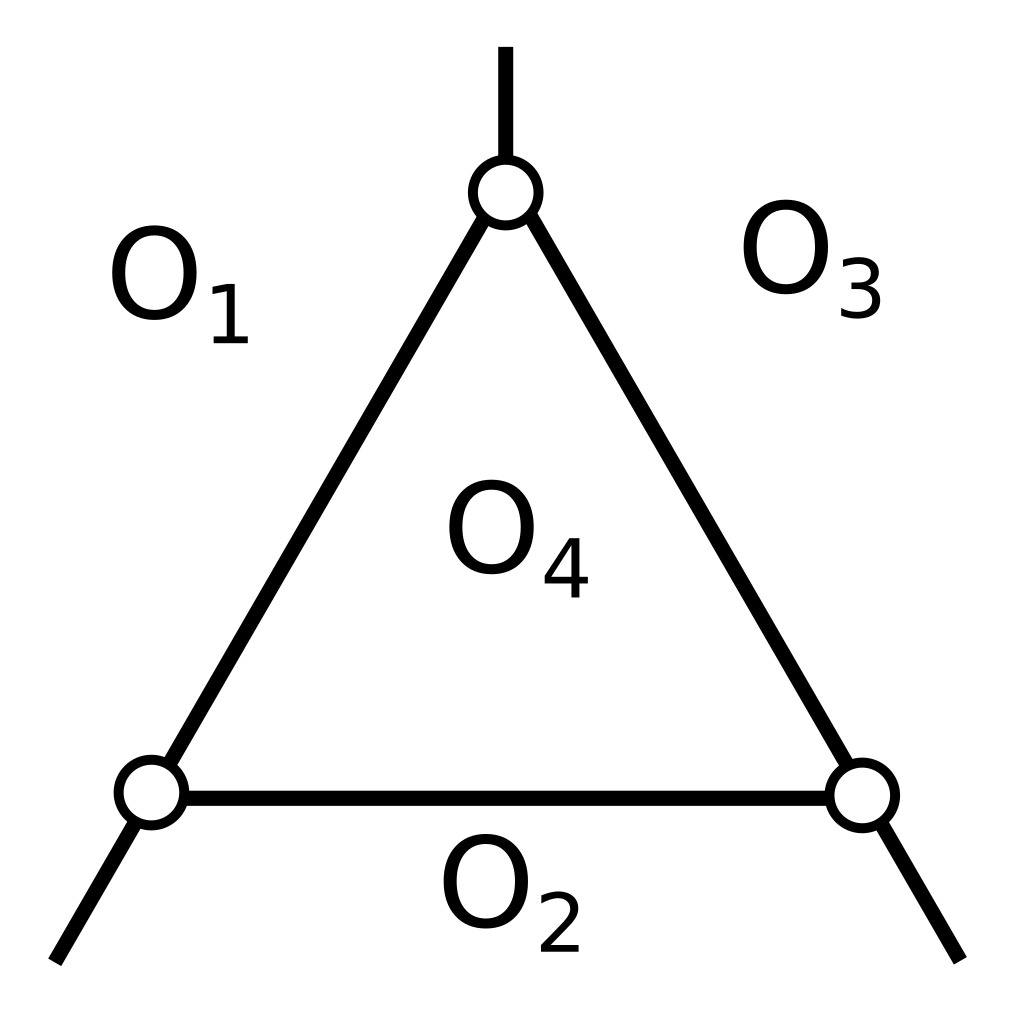
\includegraphics[width=1in, keepaspectratio]{./img/HexahedraWithSphericalFaces/tetrahedron/faces.jpg}
   \caption{Polyhedral structure.}
   \label{fig:tetrahedronFaces}
  \end{minipage}
 \hspace*{\fill}
 \end{figure}

\begin{figure}[h!tbp]
  \begin{minipage}[t]{0.23\textwidth}
   \centering
   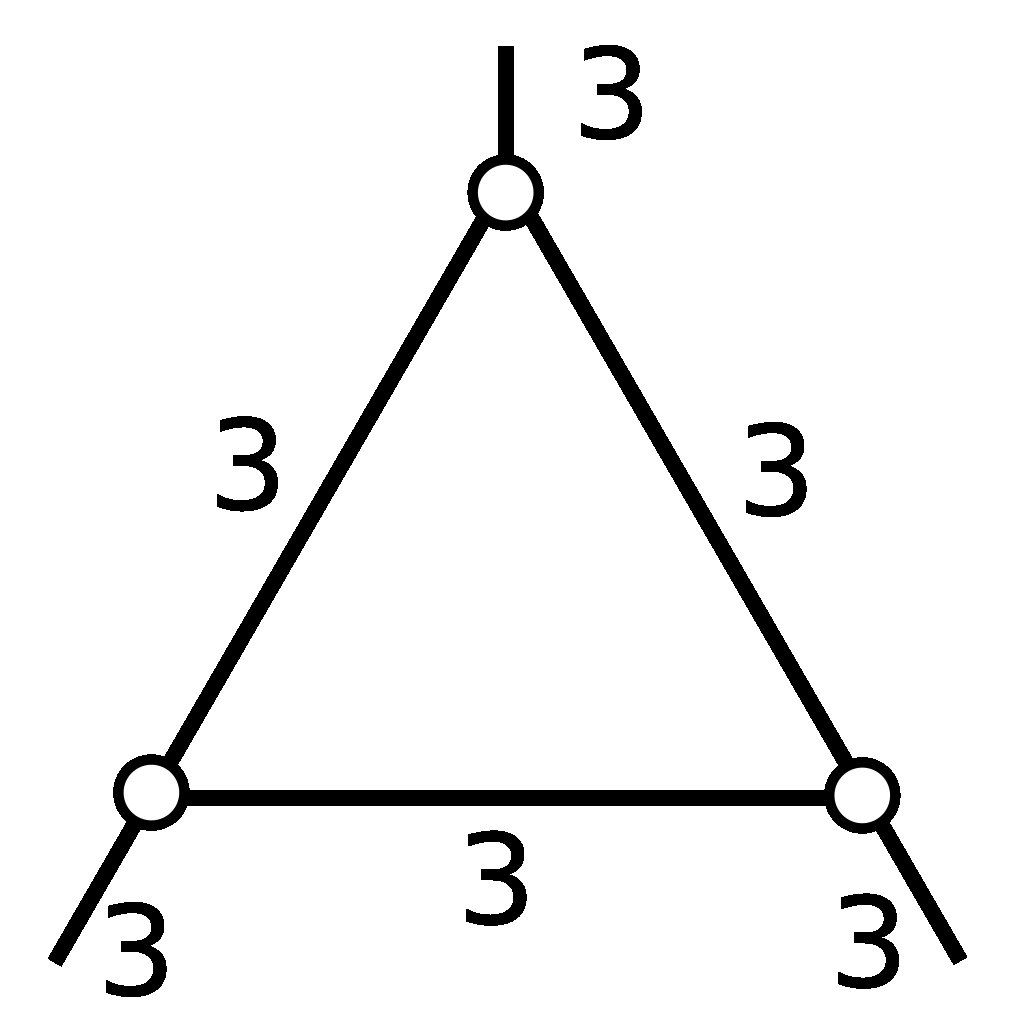
\includegraphics[width=1in,
   keepaspectratio]{./img/HexahedraWithSphericalFaces/tetrahedron/a.jpg}
   \subcaption{Type 1}
   \label{fig:tetrahedronType1}
  \end{minipage}
  \hspace*{\fill}
  \begin{minipage}[t]{0.23\textwidth}
   \centering
   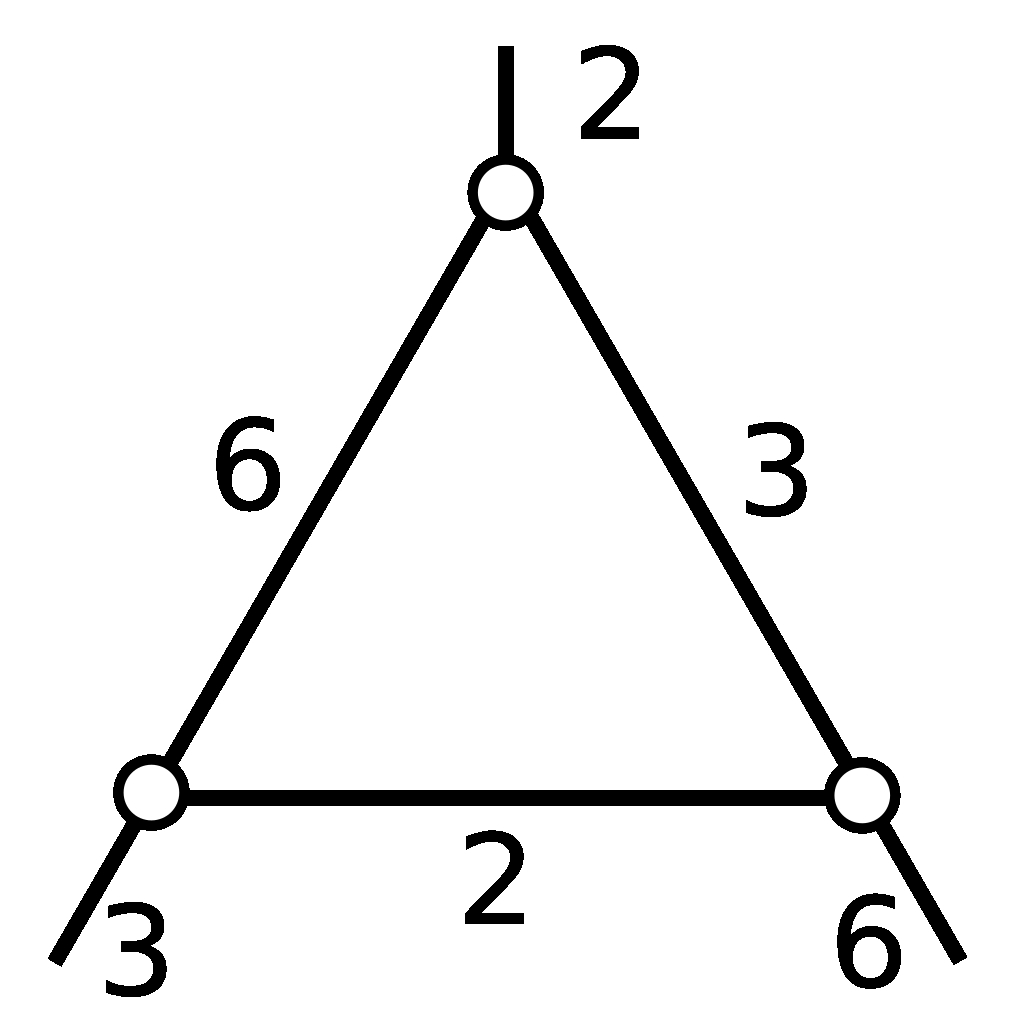
\includegraphics[width=1in, keepaspectratio]{./img/HexahedraWithSphericalFaces/tetrahedron/b.jpg}
   \subcaption{Type 2}
   \label{fig:tetrahedronType2}
  \end{minipage}
 \hspace*{\fill}
  \begin{minipage}[t]{0.23\textwidth}
   \centering
   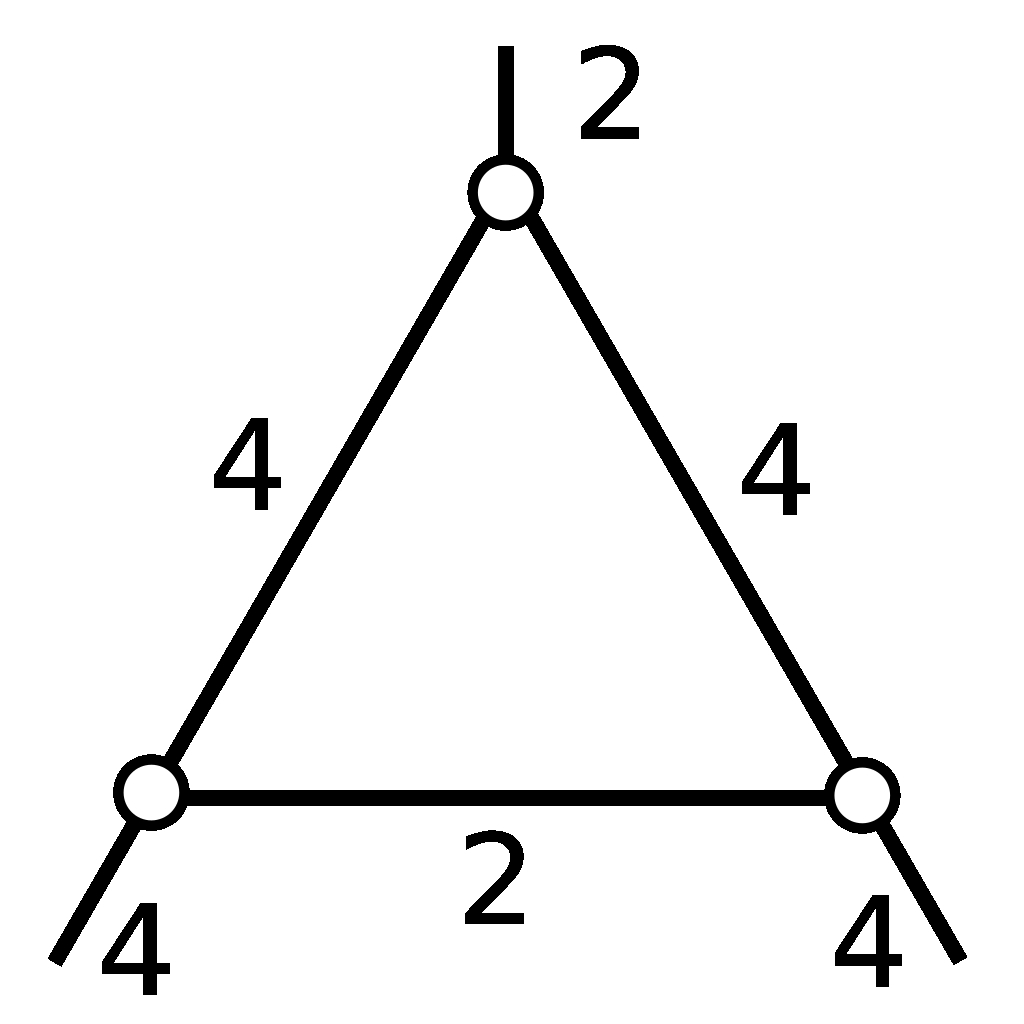
\includegraphics[width=1in, keepaspectratio]{./img/HexahedraWithSphericalFaces/tetrahedron/c.jpg}
   \subcaption{Type 3}
   \label{fig:tetrahedronType3}
  \end{minipage}
 \hspace*{\fill}
 \caption{Types of combinations of dihedral angles.}
 \label{fig:tetrahedronCombinations}
\end{figure}

\begin{figure}[h!tbp]
  \begin{minipage}[t]{0.23\textwidth}
   \centering
   
\includegraphics[width=1.3in,
   keepaspectratio]{./img/sphairahedron/tetrahedron/sphairahedronInf.jpg}
   \subcaption{}
   \label{fig:tetrahedronInf}
  \end{minipage}
  \hspace*{\fill}
  \begin{minipage}[t]{0.23\textwidth}
   \centering
   \includegraphics[width=1.3in, keepaspectratio]{./img/sphairahedron/tetrahedron/limitsetInf.jpg}
   \subcaption{}
   \label{fig:tetrahedronLimitInf}
  \end{minipage}
 \hspace*{\fill}
  \begin{minipage}[t]{0.23\textwidth}
   \centering
   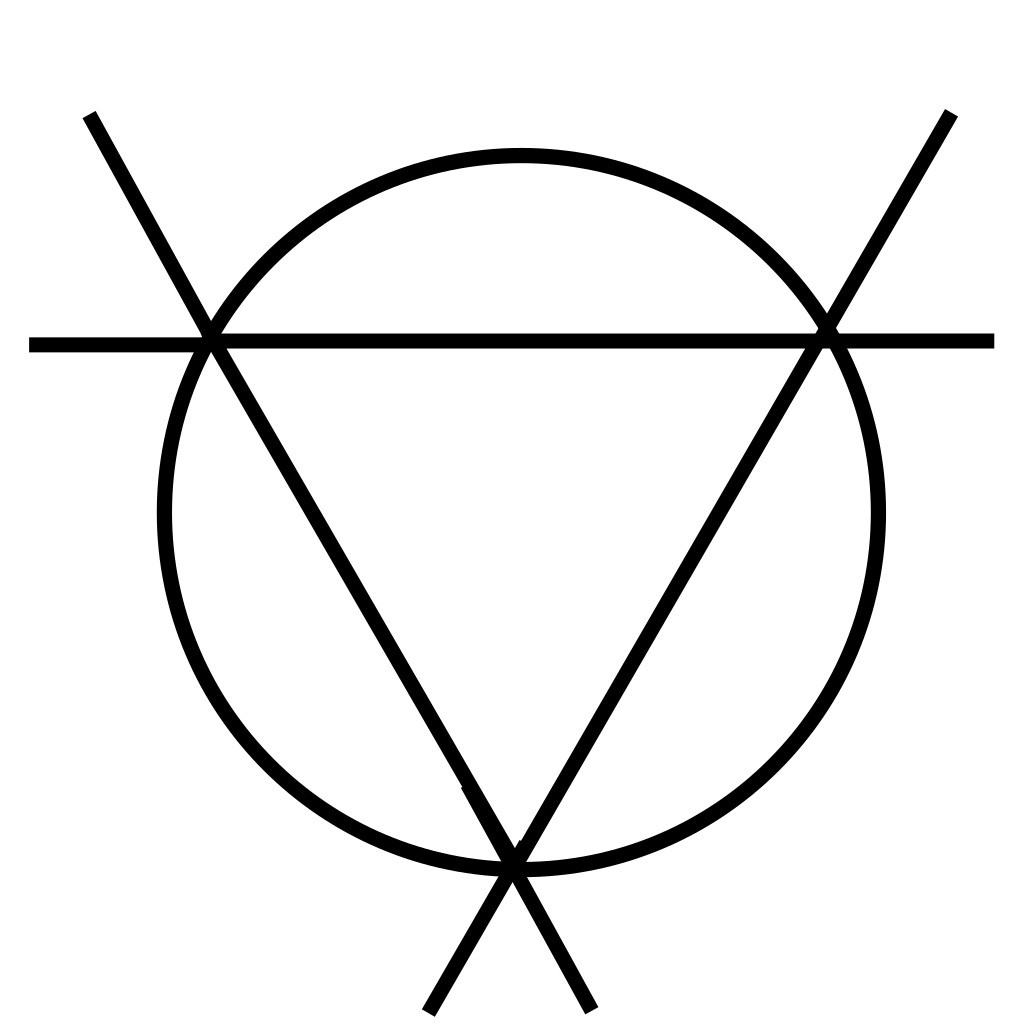
\includegraphics[width=1.3in, keepaspectratio]{./img/HexahedraWithSphericalFaces/tetrahedron/slice_a.jpg}
   \subcaption{}
   \label{fig:tetrahedronSliceA}
  \end{minipage}
 \hspace*{\fill}
  \begin{minipage}[t]{0.23\textwidth}
   \centering
   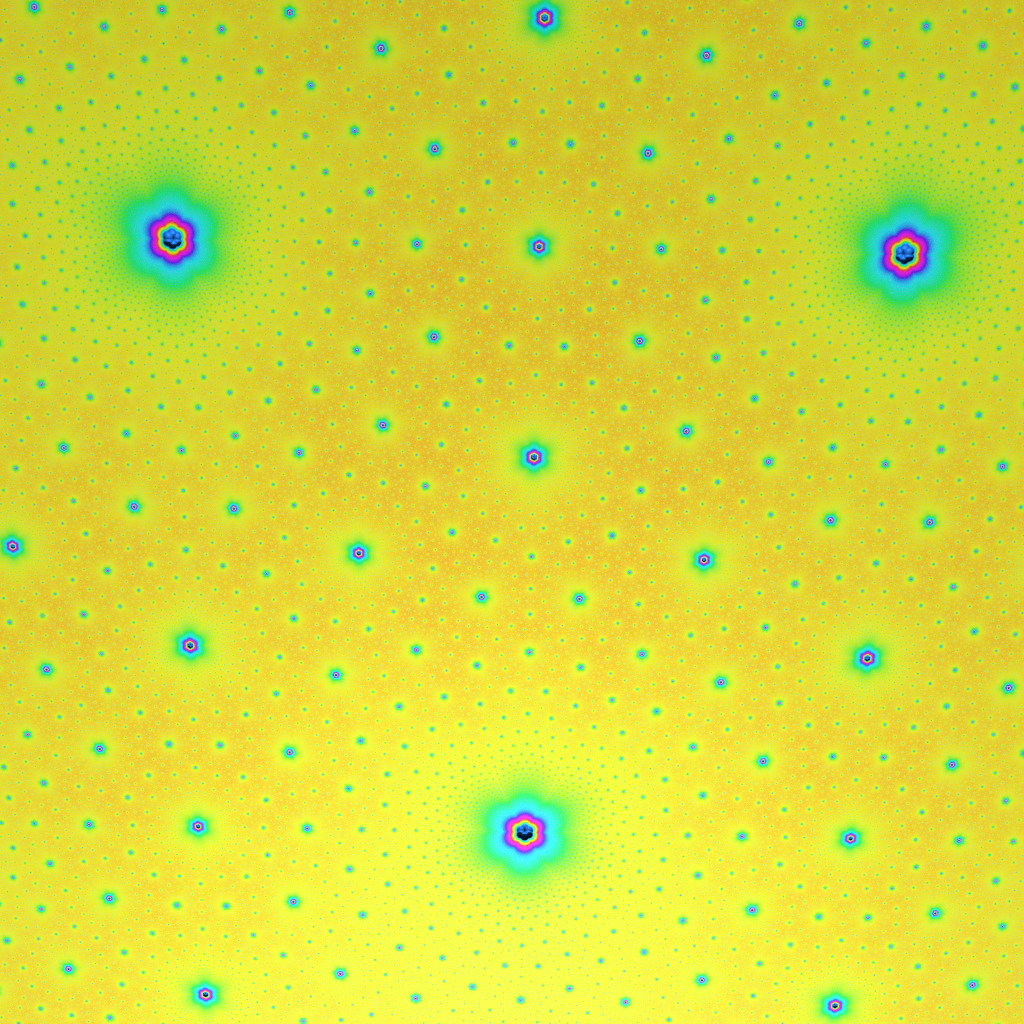
\includegraphics[width=1.3in, keepaspectratio]{./img/sphairahedron/tetrahedron/limitsetAbove_a.jpg}
   \subcaption{}
   \label{fig:tetrahedronLimitsetAboveA}
  \end{minipage}
 \hspace*{\fill}
 \caption{A tetrahedron of type 1.}
 \label{fig:tetrahedronInf_a}
\end{figure}

\begin{figure}[h!tbp]
  \begin{minipage}[t]{0.23\textwidth}
   \centering
   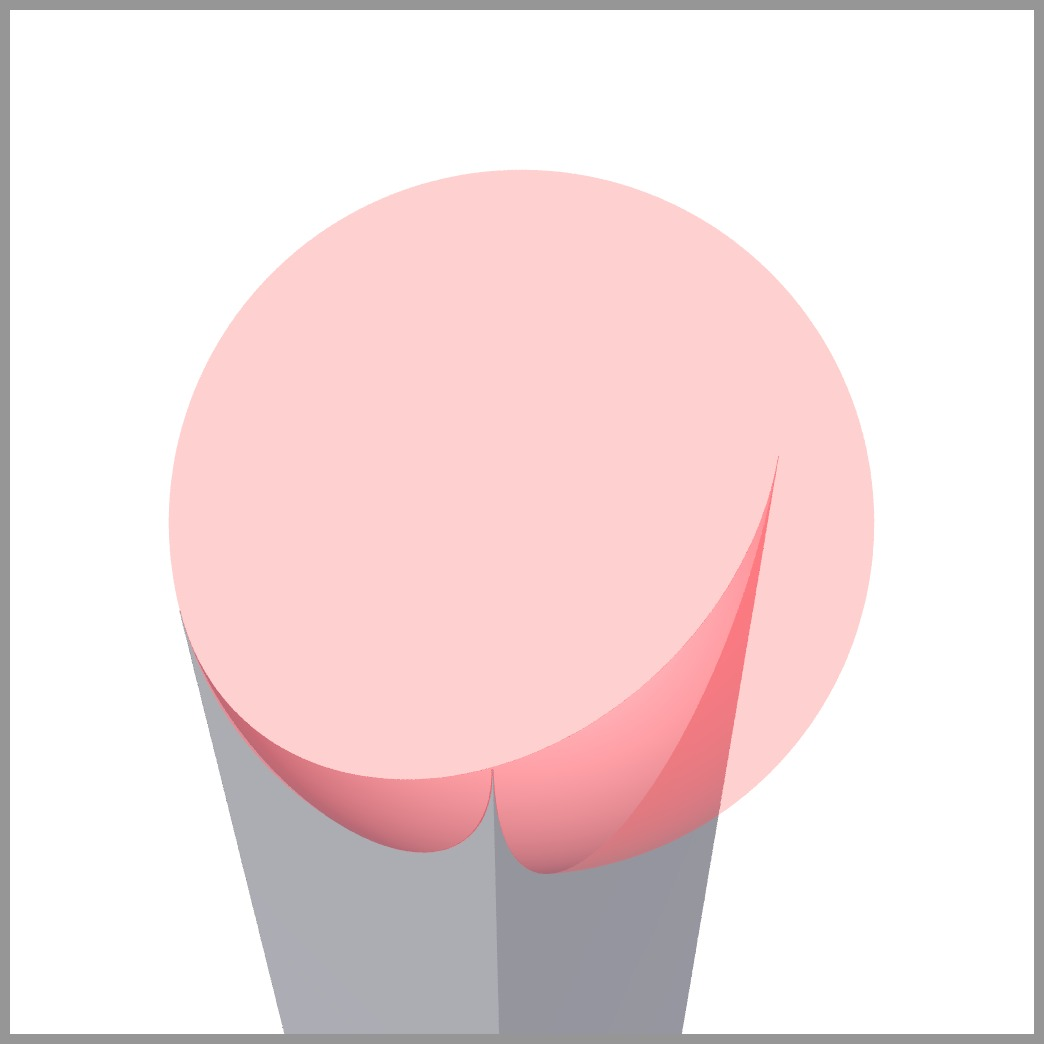
\includegraphics[width=1.3in,
   keepaspectratio]{./img/sphairahedron/tetrahedron/sphairahedralPrism_b.jpg}
   \subcaption{}
   \label{fig:tetrahedronPrismInf_b}
  \end{minipage}
  \hspace*{\fill}
  \begin{minipage}[t]{0.23\textwidth}
   \centering
   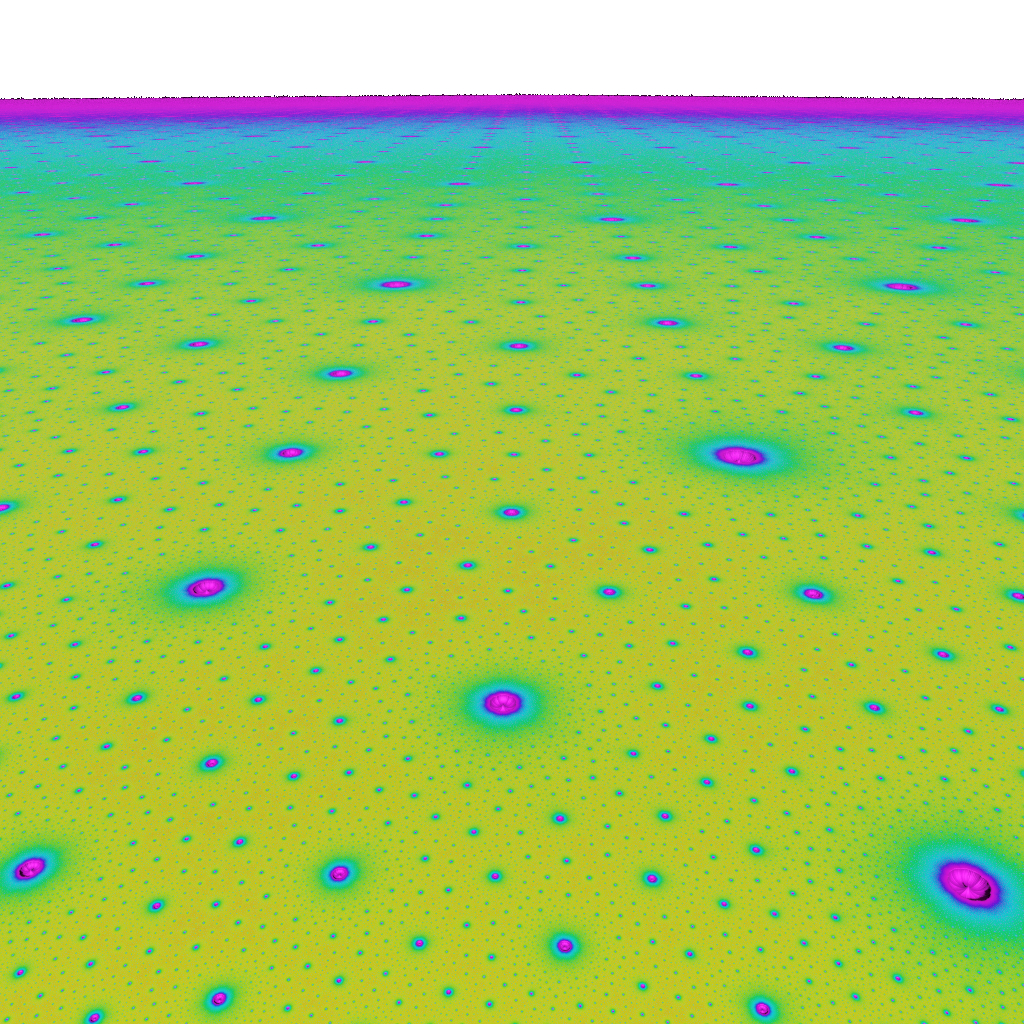
\includegraphics[width=1.3in, keepaspectratio]{./img/sphairahedron/tetrahedron/limitset_b.jpg}
   \subcaption{}
   \label{fig:tetrahedronLimitsetInf_b}
  \end{minipage}
 \hspace*{\fill}
  \begin{minipage}[t]{0.23\textwidth}
   \centering
   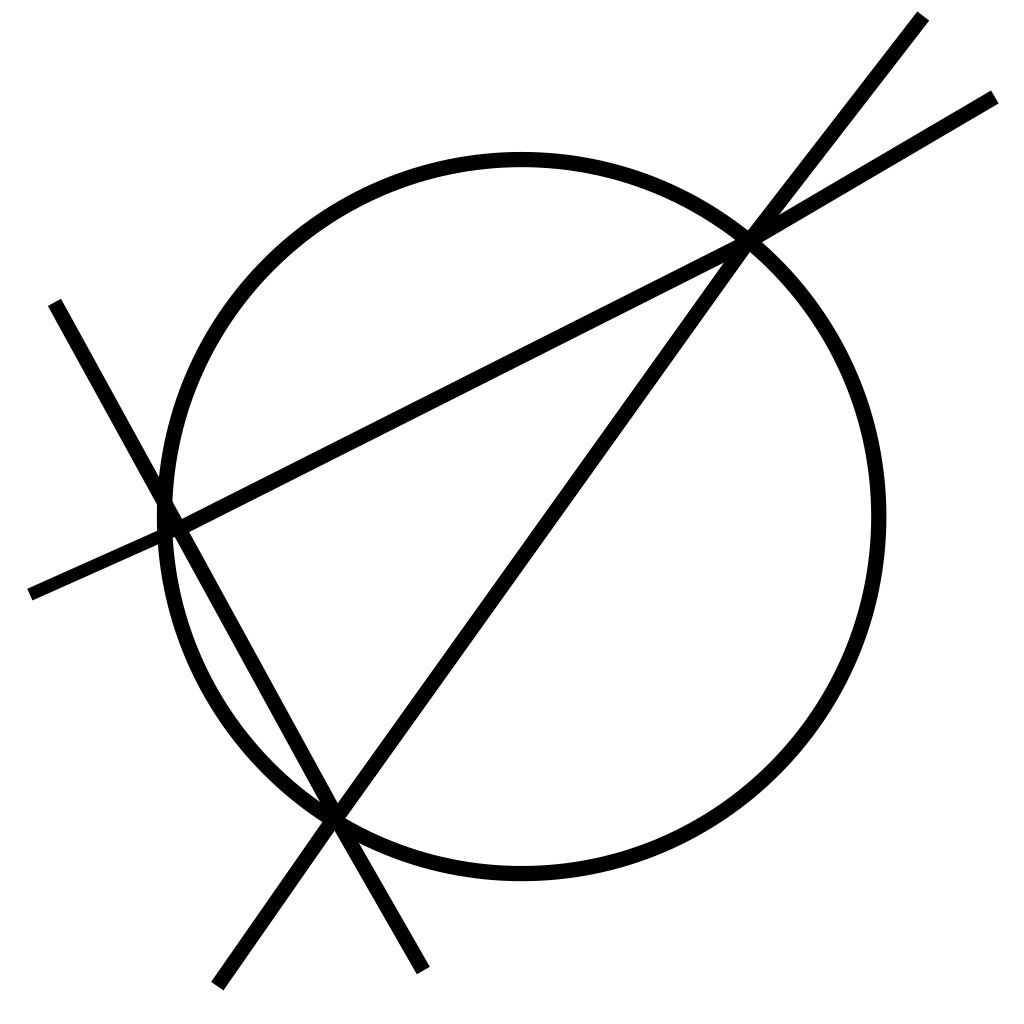
\includegraphics[width=1.3in, keepaspectratio]{./img/HexahedraWithSphericalFaces/tetrahedron/slice_b.jpg}
   \subcaption{}
   \label{fig:tetrahedronSlice_b}
  \end{minipage}
 \hspace*{\fill}
  \begin{minipage}[t]{0.23\textwidth}
   \centering
   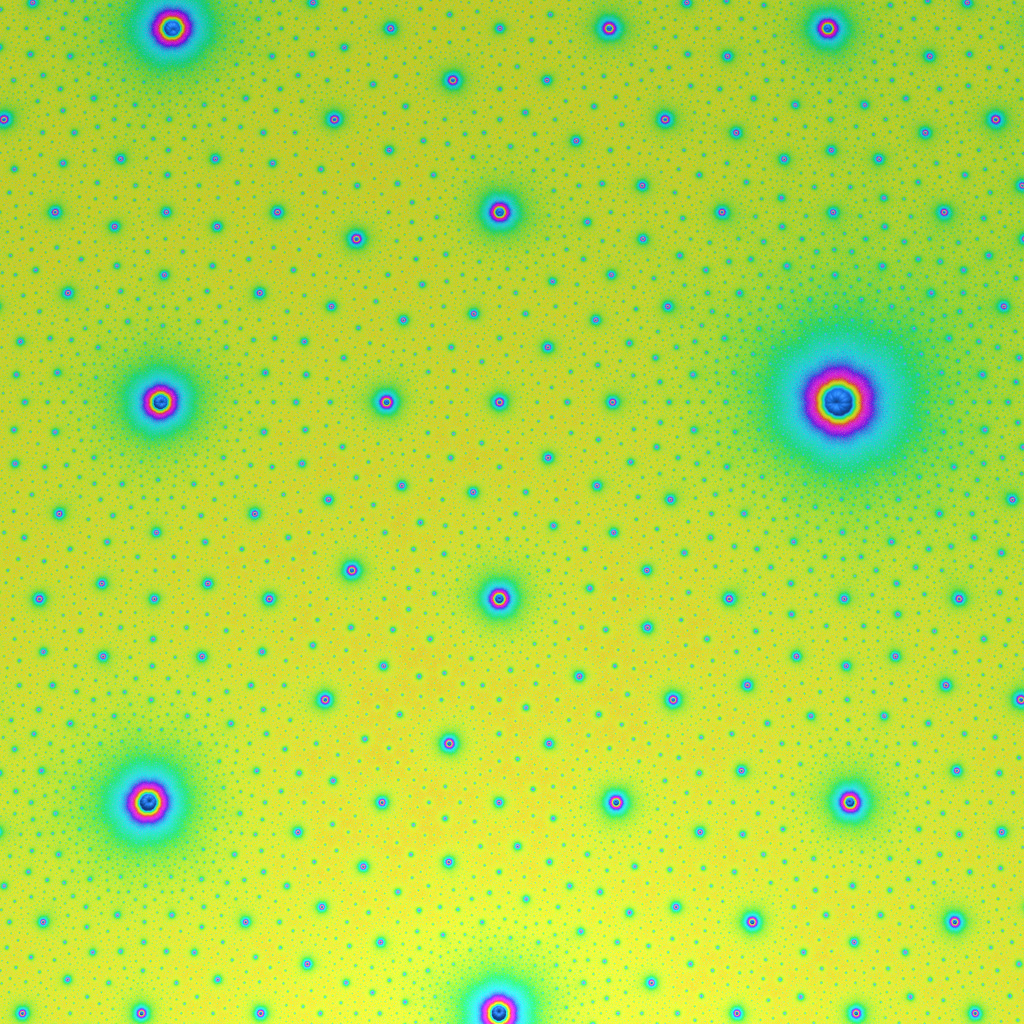
\includegraphics[width=1.3in, keepaspectratio]{./img/sphairahedron/tetrahedron/limitsetAbove_b.jpg}
   \subcaption{}
   \label{fig:tetrahedronAbove_b}
  \end{minipage}
 \hspace*{\fill}
 \caption{A tetrahedron of type 2.}
 \label{fig:tetrahedronInf_b}
\end{figure}

\begin{figure}[h!tbp]
  \begin{minipage}[t]{0.23\textwidth}
   \centering
   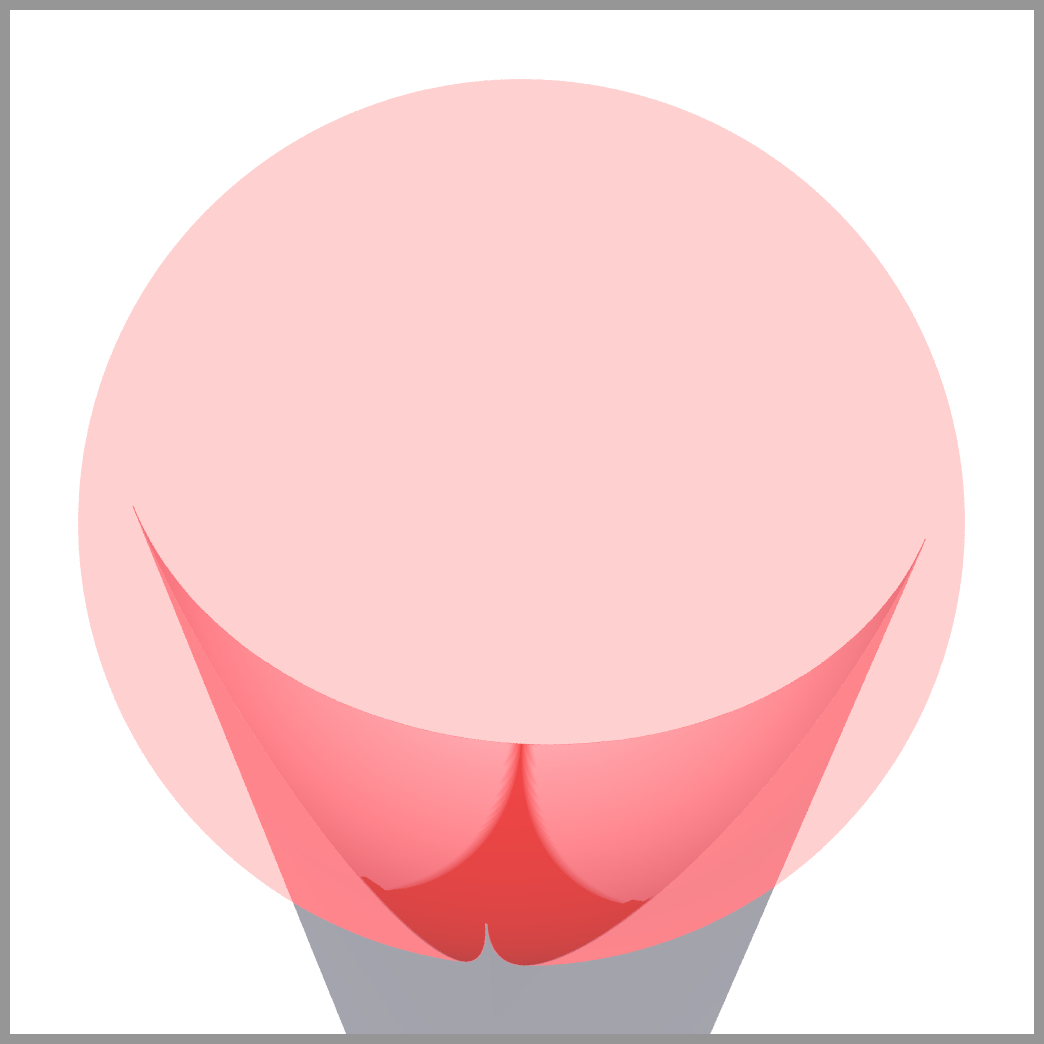
\includegraphics[width=1.3in,
   keepaspectratio]{./img/sphairahedron/tetrahedron/sphairahedralPrism_c.jpg}
   \subcaption{}
   \label{fig:tetrahedralPrism_c}
  \end{minipage}
  \hspace*{\fill}
  \begin{minipage}[t]{0.23\textwidth}
   \centering
   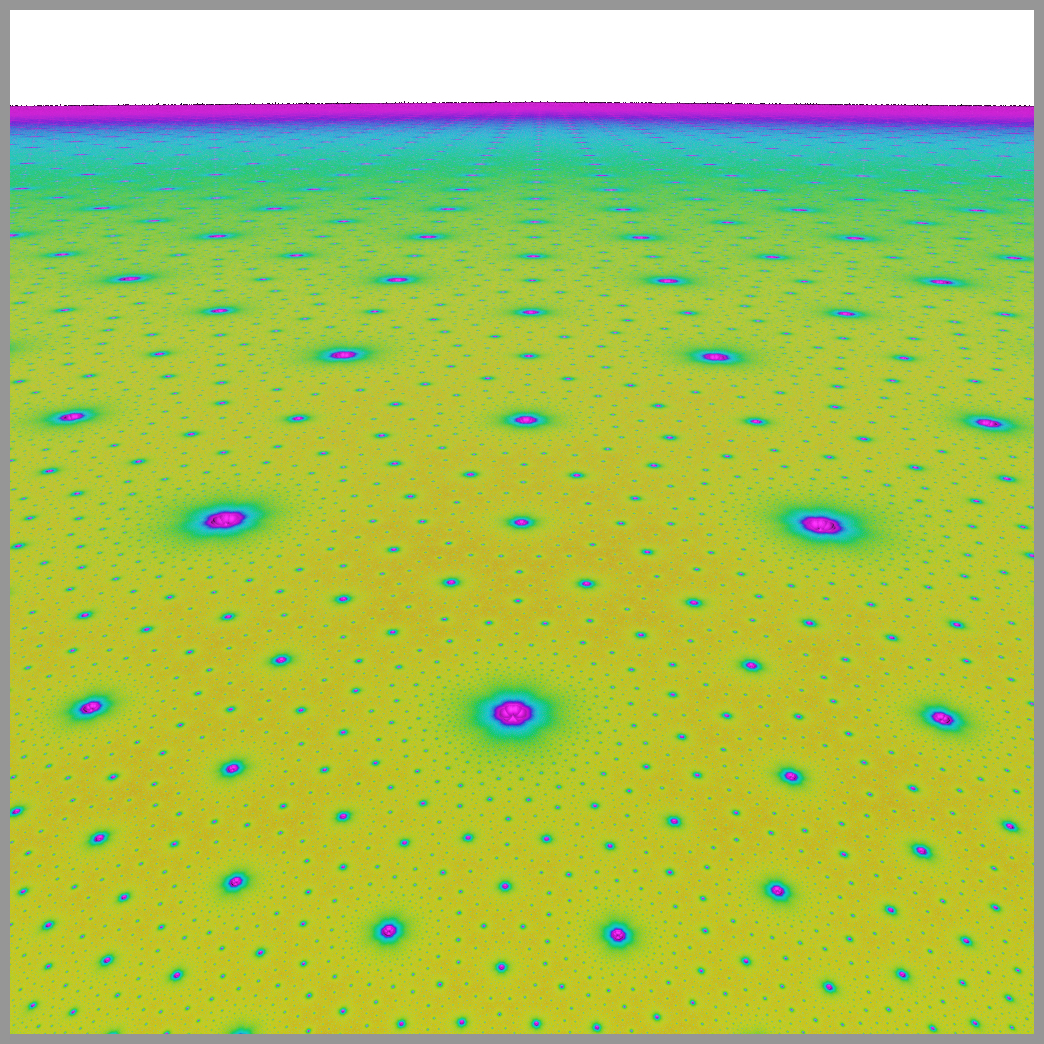
\includegraphics[width=1.3in, keepaspectratio]{./img/sphairahedron/tetrahedron/limitset_c.jpg}
   \subcaption{}
   \label{fig:tetrahedronLimitset_c}
  \end{minipage}
 \hspace*{\fill}
  \begin{minipage}[t]{0.23\textwidth}
   \centering
   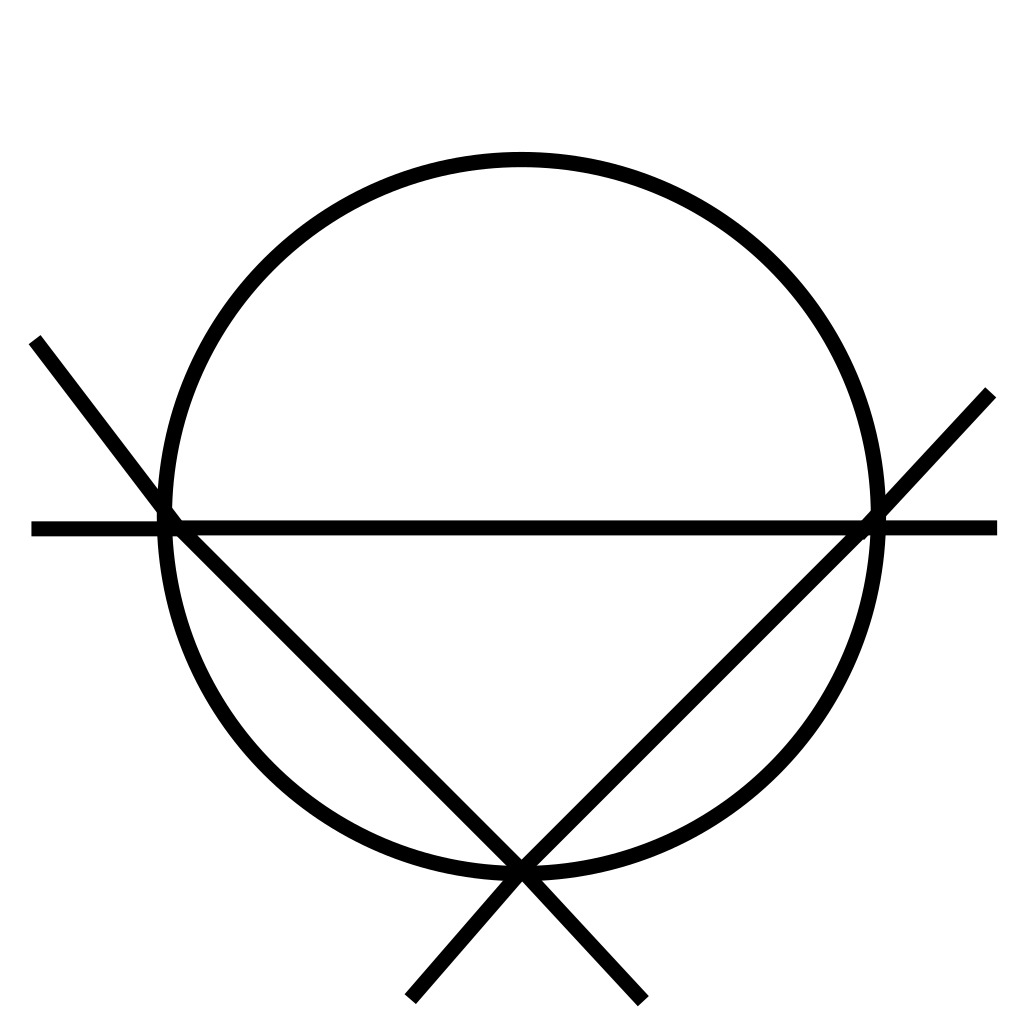
\includegraphics[width=1.3in, keepaspectratio]{./img/HexahedraWithSphericalFaces/tetrahedron/slice_c.jpg}
   \subcaption{}
   \label{fig:tetrahedronSlice_c}
  \end{minipage}
 \hspace*{\fill}
  \begin{minipage}[t]{0.23\textwidth}
   \centering
   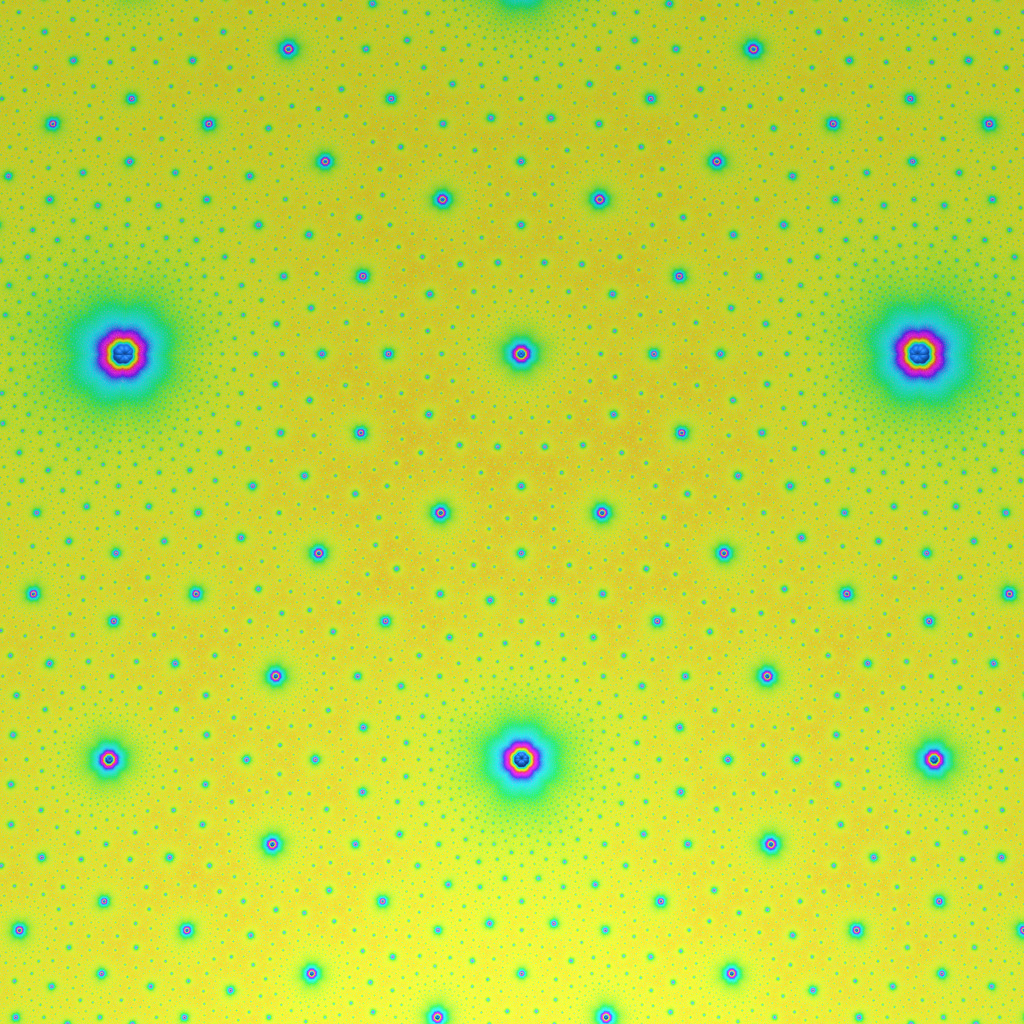
\includegraphics[width=1.3in, keepaspectratio]{./img/sphairahedron/tetrahedron/limitsetAbove_c.jpg}
   \subcaption{}
   \label{fig:tetrahedronAbove_c}
  \end{minipage}
 \hspace*{\fill}
 \caption{A tetrahedron of type 3.}
 \label{fig:tetrahedronInf_c}
\end{figure}

\begin{figure}[h!tbp]
  \begin{minipage}[t]{0.49\textwidth}
   \centering
   
\includegraphics[width=1.35in, height=1.35in, keepaspectratio]{./img/sphairahedron/tetrahedron/sphairahedronFinite.jpg}
   \subcaption{Sphairahedron}
   \label{fig:tetrahedronFiniteSphairahedron}
  \end{minipage}
  \hspace*{\fill}
  \begin{minipage}[t]{0.49\textwidth}
   \centering
   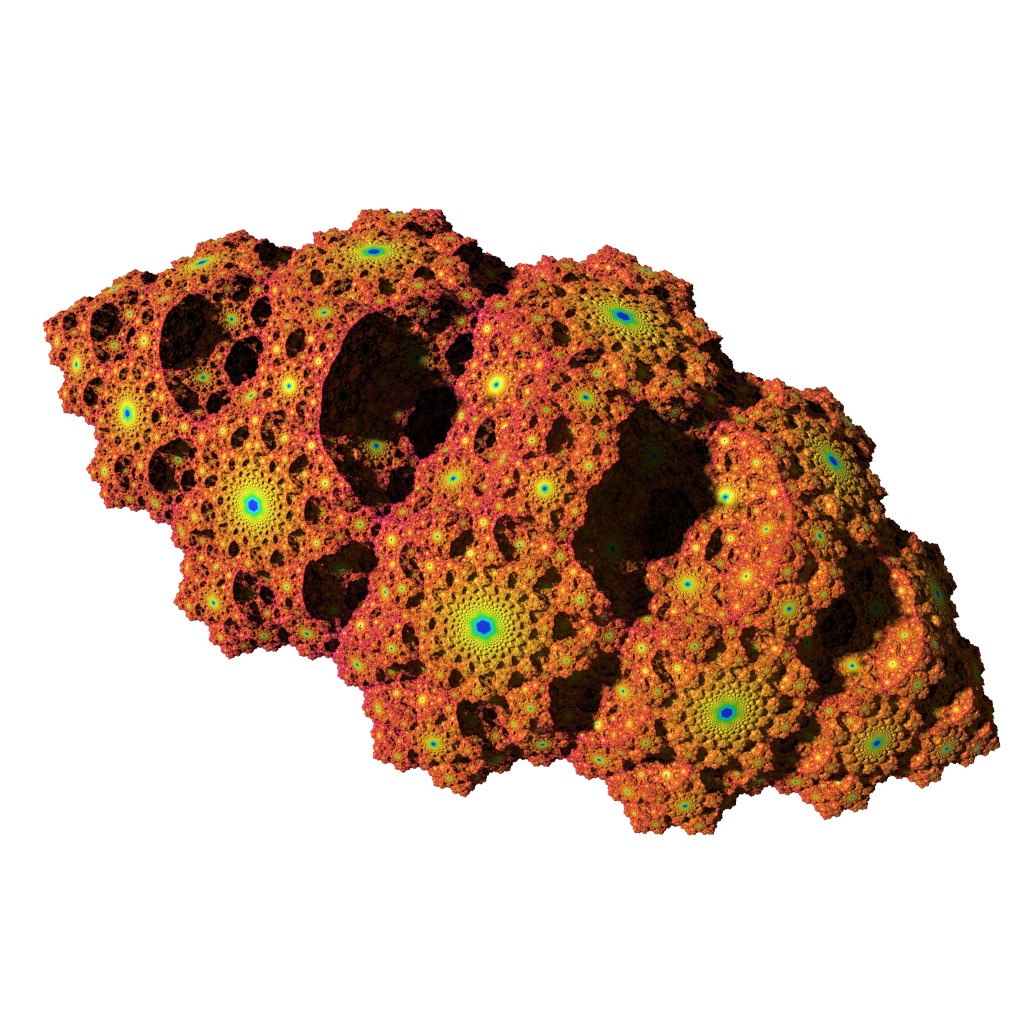
\includegraphics[width=1.35in, height=1.35in, keepaspectratio]{./img/sphairahedron/tetrahedron/limitsetFinite.jpg}
   \subcaption{Limit set}
   \label{fig:tetrahedronFiniteLimitset}
  \end{minipage}
  \hspace*{\fill}
  \caption{A finite tetrahedron of type 1.}
  \label{fig:tetrahedronFinite}
\end{figure}

% end of figs of tetrahedron

A tetrahedron (Figure \ref{fig:tetrahedron}) has a polyhedral structure as shown in Figure \ref{fig:tetrahedronFaces}.  It is a sphairahedron with fewest faces.
There are three types of combinations of dihedral angles of edges as shown in
Figure \ref{fig:tetrahedronCombinations}.

\begin{proposition}\label{prop:paraSpace_Tetrahedron}
In each type of the dihedral angles, the parameter space consists of one point.
\end{proposition}

\begin{proof}   Suppose that one of the vertices of the sphairahedron is the infinite-point $\infty$.  In the type (a) case, the neighborhood of the infinite vertex is a regular triangle prism.  It is because all dihedral angles equal to $\frac{\pi}{3}$.  Without loss of generality, we may assume the followings.
\begin{align*}
\overline{D_1}&=\{(x,y,z) \mid 1 \le x \} \cup\{\infty\}\\
\overline{D_2}&=\{(x,y,z) \mid 1 \le -\frac{1}{2}x+\frac{\sqrt{3}}{2}y \} \cup\{\infty\}\\
\overline{D_3}&=\{(x,y,z) \mid 1 \le -\frac{1}{2}x-\frac{\sqrt{3}}{2}y \} \cup\{\infty\}\\
\overline{D_4}&=\{(x,y,z) \mid (x-x_4)^2+(y-y_4)^2+(z-z_4)^2 \le r_4^2\} \\
O_i & = \partial(\overline{D_i}) \qquad(i=1, 2, 3, 4.)
\end{align*}

$S^3\setminus(\overline{D_1} \cup \overline{D_2} \cup \overline{D_3})$ is the infinite triangle prism.  Let a vertex $P_{ijk}$ be $O_i \cap O_j \cap O_k$. (Generally, if the intersection of three spheres is not empty, then it consists of inifinity number of points or two points or one point.  In our case, the condition that the sphairahedron is ideal, the intersection is a point.) From Lemma \ref{lemma:equivalentOfSH}, we may assume that $P_{124}=(1,\sqrt{3}, 0)$.  Using Lemma \ref{lemma:CenterOfSphere}(1), we have $z_4=0$ and hence $P_{234}=(-2, 0, 0)$ and $P_{134}=(1, -\sqrt{3}, 0)$.  The equation $\sqrt{3}x_4 -y_4=0$ follows \ref{lemma:CenterOfSphere}(3) and $P_{124}=(1,\sqrt{3}, 0)$.  Thus we have that the center of $O_4$ is the origin and
\[
\overline{D_4}=\{(x,y,z) \mid x^2+y^2+z^2 \le 3 \}.
\]
This means that the parameter space of $\overline{D_i}$'s consists of one point.  In case of another type, we show it in the same way.
\end{proof}

Figures  \ref{fig:tetrahedronInf_a}(a), \ref{fig:tetrahedronInf_b}(a),
and \ref{fig:tetrahedronInf_c}(a) show the rendered pictures of the sphairahedra of type 1, 2, and 3 respectively.

\begin{proposition} \label{prop:tetrahedronLimitSet}
Assume that the tetrahedron $T$ has the infinite vertex.  In any case of dihedral angles, the limit set is the union of a plane and $\infty$.
\end{proposition}

\begin{proof}
We show it in case of the type (a).  Let $\overline{D_i}$'s be as in the proof of Proposition \ref{prop:paraSpace_Tetrahedron}.  The tetrahedron $T$ is given by
\[
T = \{(x,y,z) \mid z<0\} \setminus(\overline{D_1} \cup \overline{D_2} \cup \overline{D_3} \cup \overline{D_4}).
\]
See Figure \ref{fig:tetrahedronInf_a}(a).  If we regard the lower half plane $\{(x,y,z) \mid z<0\}$ as the hyperbolic space $\mathbb{H}^3$, $T$ is a hyperbolic ideal tetrahedron, because all edges are perpendicular to the $xy$-plane.  For the tiling $L=(T,G)$, the boundary of the total tiling space $\cup_k |L|_k$
coincides to $\partial{\mathbb{H}^3}$ and the limit set is the $xy$-plane.
\end{proof}

Indeed, the quasi-spheres are shown in Figures \ref{fig:tetrahedronInf_a}(b), \ref{fig:tetrahedronInf_b}(b),
and \ref{fig:tetrahedronInf_c}(b).  They are $xy$-plane.  They have different colored patterns and it is because the combinations of the dihedral angles are different from each other.  These colored patterns are shown in Figures  \ref{fig:tetrahedronInf_a}(d), \ref{fig:tetrahedronInf_b}(d),
and \ref{fig:tetrahedronInf_c}(d) respectively.  These patterns are generated by reflections of three straight lines and one circle shown in Figures \ref{fig:tetrahedronInf_a}(c), \ref{fig:tetrahedronInf_b}(c),
and \ref{fig:tetrahedronInf_c}(c) respectively.  See more in Section \ref{section:patternsOfPlanes}. The tiling group $G$ of $T$ is 3-Kleinian.  If a tetrahedron is finite, the limit set is a sphere as seen in Figure \ref{fig:tetrahedronFinite}.

%%% 3. 3 %%
\subsection{Pentahedron}

\subsubsection{Classification of pentahedra}

There are two polyhedral structures of pentahedra. One is a quadrangular pyramid (Figure \ref{fig:quadrangularPyramid}) and the other is a triangular prism (Figure \ref{fig:triangularPrism}.)

\subsubsection{Quadrangular pyramid}

\begin{figure}[h!tbp]
  \begin{minipage}[t]{0.5\textwidth}
   \centering
   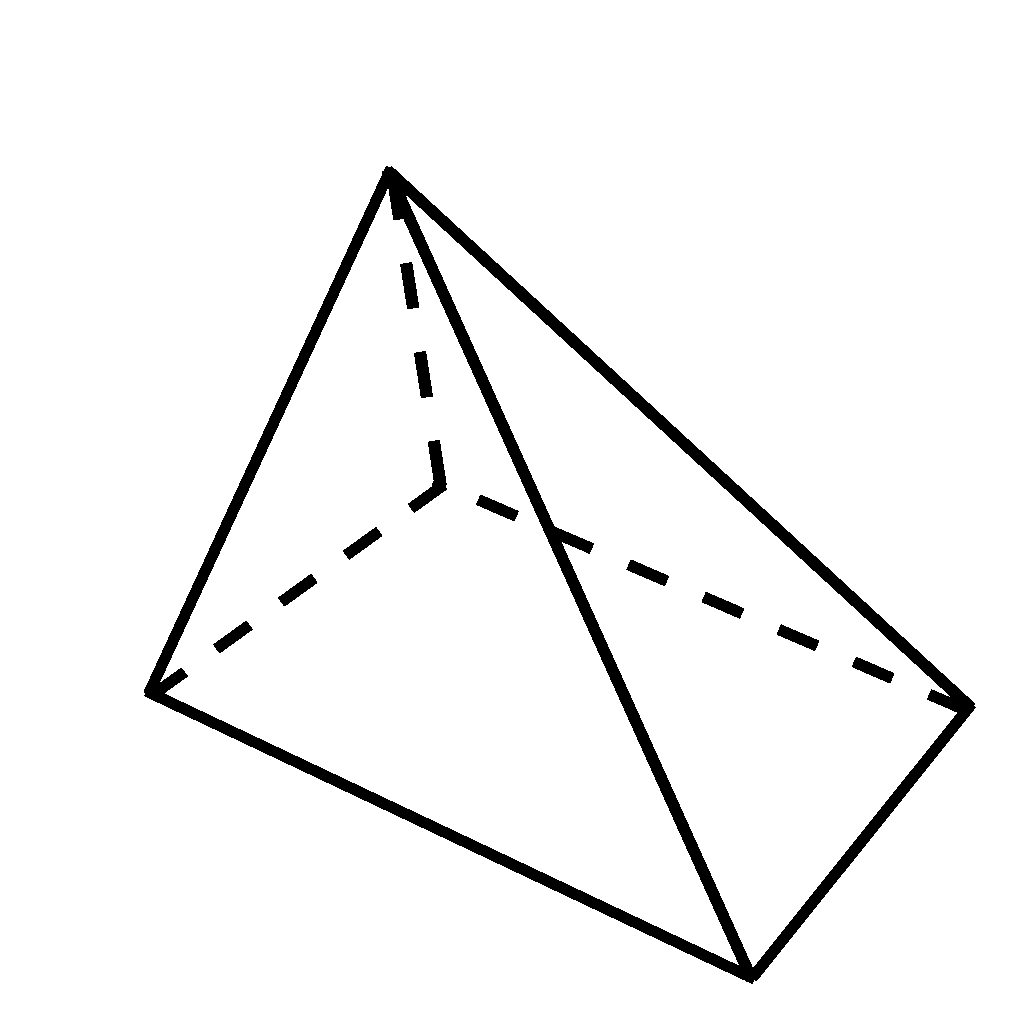
\includegraphics[width=1in, keepaspectratio]{./img/HexahedraWithSphericalFaces/pentahedralPyramid/pyramid.jpg}
   \caption{Quadrangular pyramid.}
   \label{fig:quadrangularPyramid}
  \end{minipage}
 \hspace*{\fill}
  \begin{minipage}[t]{0.5\textwidth}
   \centering
   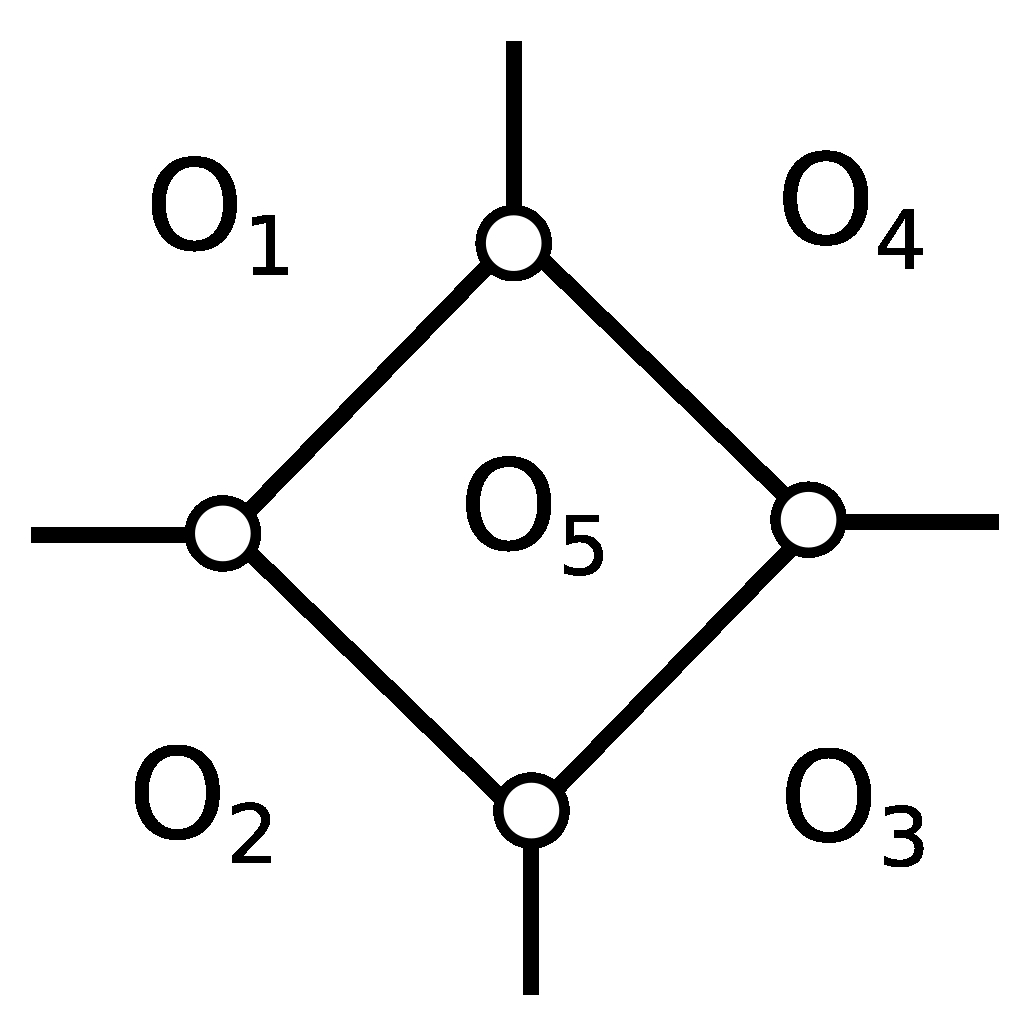
\includegraphics[width=1in, keepaspectratio]{./img/HexahedraWithSphericalFaces/pentahedralPyramid/faces.jpg}
   \caption{Polyhedral structures.}
   \label{fig:quadrangularPyramidFaces}
  \end{minipage}
 \hspace*{\fill}
\end{figure}

\begin{figure}[h!tbp]
 \hspace*{\fill}
 \begin{minipage}[t]{0.24\textwidth}
   \centering
   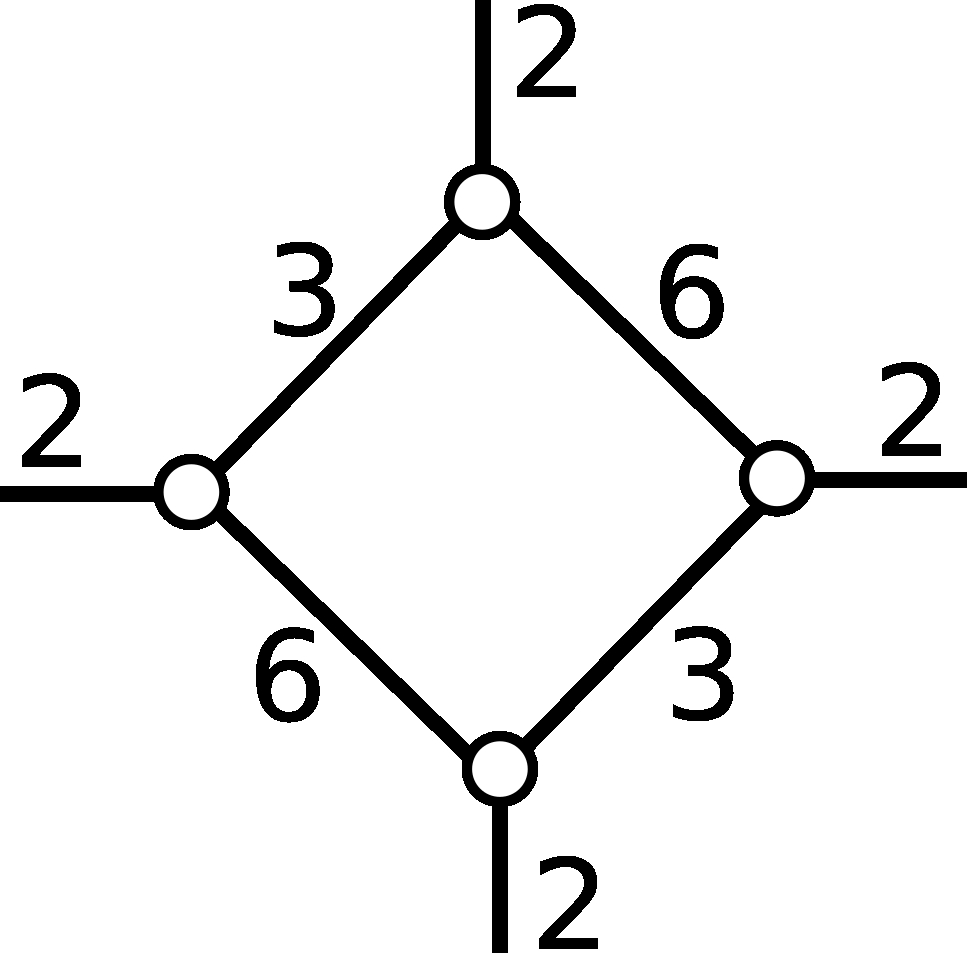
\includegraphics[width=1in,
   keepaspectratio]{./img/HexahedraWithSphericalFaces/pentahedralPyramid/a.jpg}
   \subcaption{Type 1}
   \label{fig:quadrangularPyramid1}
 \end{minipage}
 \hspace*{\fill}
 \begin{minipage}[t]{0.24\textwidth}
   \centering
   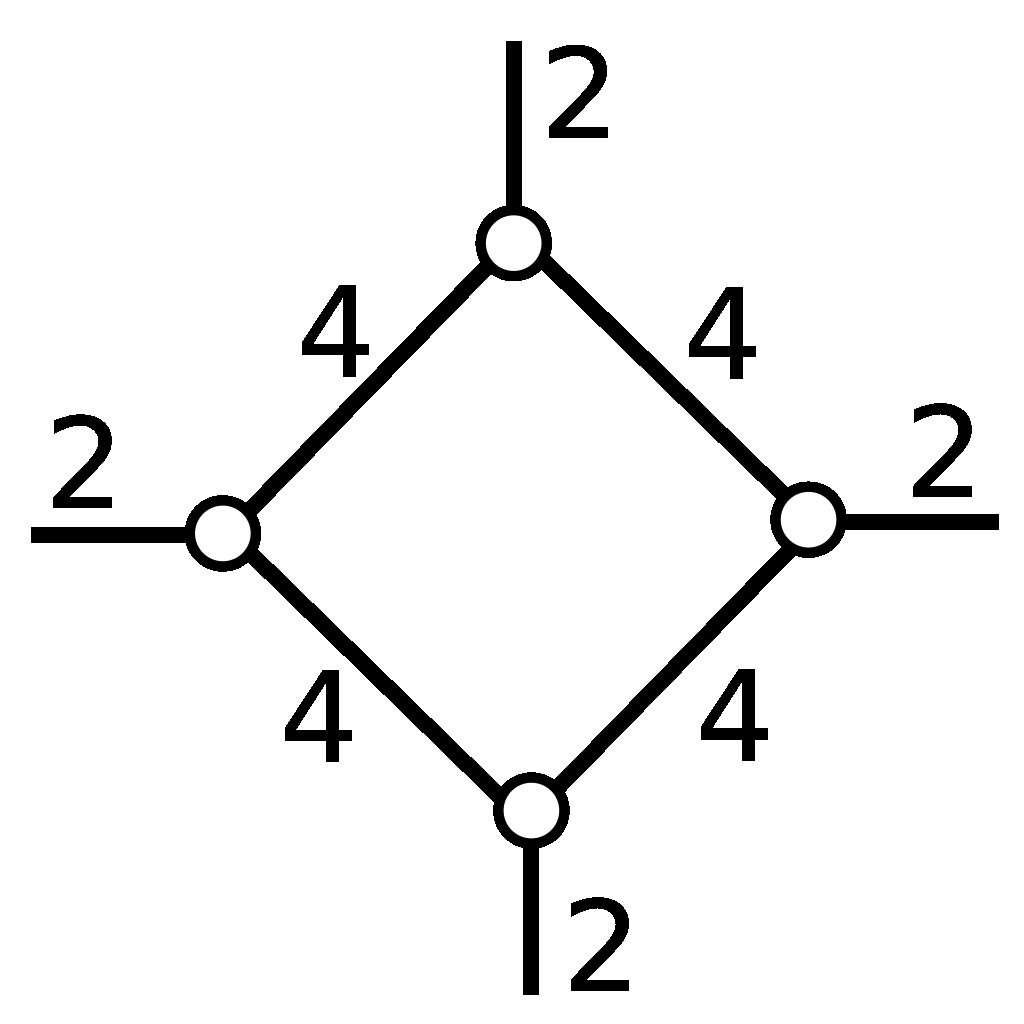
\includegraphics[width=1in, keepaspectratio]{./img/HexahedraWithSphericalFaces/pentahedralPyramid/b.jpg}
   \subcaption{Type 2}
   \label{fig:quadrangularPyramid2}
 \end{minipage}
 \hspace*{\fill}
 \caption{Types of combinations of dihedral angles.}
  \label{fig:quadrangularPyramidCombinations}
\end{figure}

\begin{figure}[h!tbp]
   \centering
   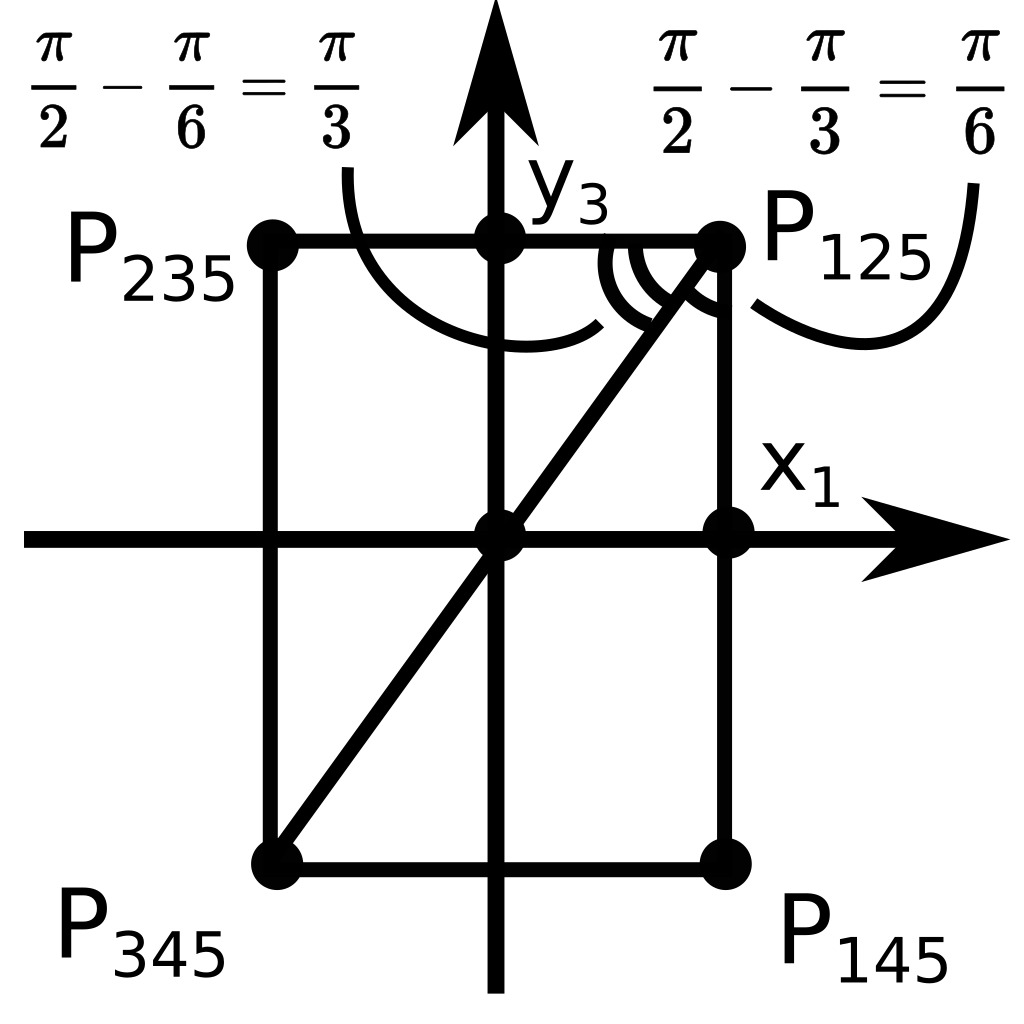
\includegraphics[width=1.5in, keepaspectratio]{./img/HexahedraWithSphericalFaces/pentahedralPyramid/proofQuadrangularPyramid.jpg}
   \caption{Section at $z=0$.}
   \label{fig:quadrangularPyramidAtOrigin}
 \hspace*{\fill}
\end{figure}

\begin{figure}[h!tbp]
  \begin{minipage}[t]{0.23\textwidth}
   \centering 
\includegraphics[width=1.3in,
   keepaspectratio]{./img/sphairahedron/pentahedralPyramid/sphairahedronInf.jpg}
   \subcaption{}
   \label{fig:pentahedralPyramidInf}
  \end{minipage}
  \hspace*{\fill}
  \begin{minipage}[t]{0.23\textwidth}
   \centering
   \includegraphics[width=1.3in, keepaspectratio]{./img/sphairahedron/pentahedralPyramid/limitsetInf.jpg}
   \subcaption{}
   \label{fig:pentahedralPyramidLimitset}
  \end{minipage}
 \hspace*{\fill}
  \begin{minipage}[t]{0.23\textwidth}
   \centering
   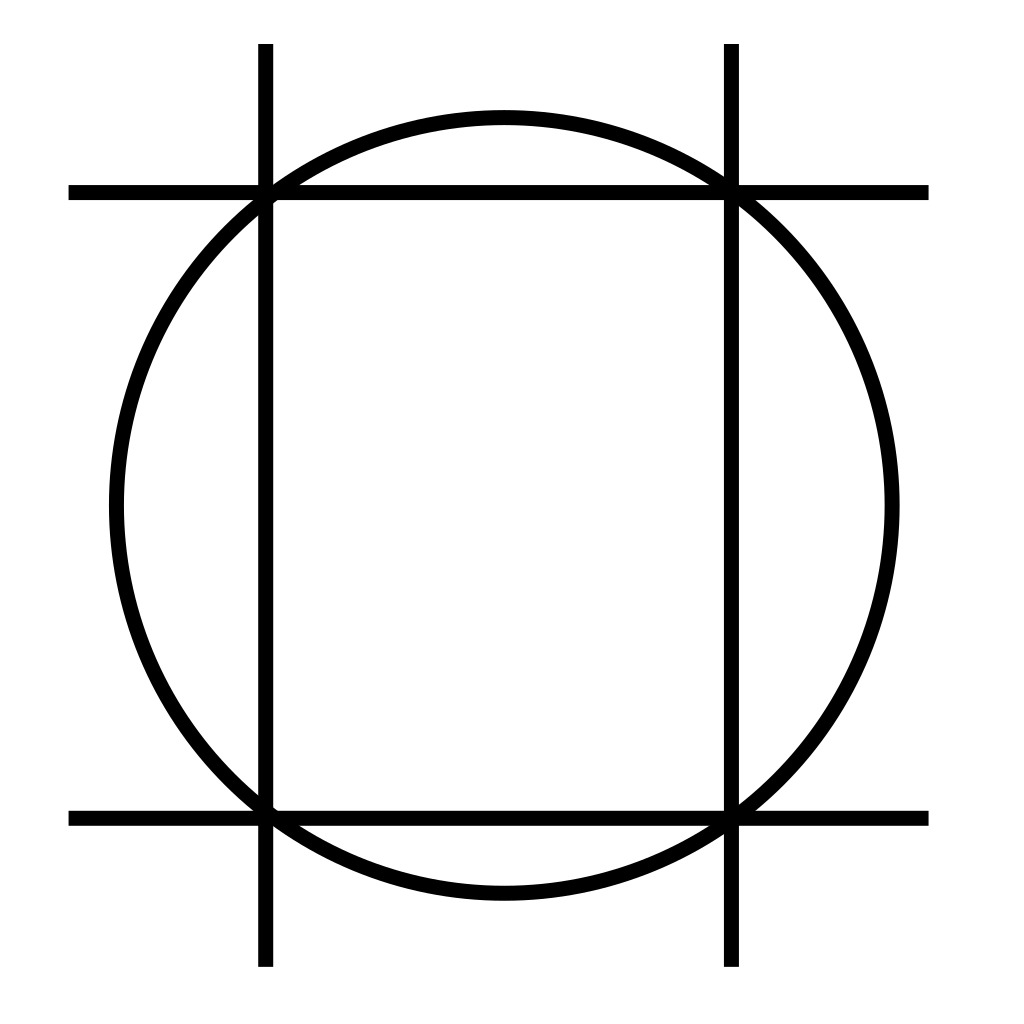
\includegraphics[width=1.3in, keepaspectratio]{./img/HexahedraWithSphericalFaces/pentahedralPyramid/slice_a.jpg}
   \subcaption{}
   \label{fig:pentahedralPyramidSlice}
  \end{minipage}
 \hspace*{\fill}
  \begin{minipage}[t]{0.23\textwidth}
   \centering
   \includegraphics[width=1.3in, keepaspectratio]{./img/sphairahedron/pentahedralPyramid/limitsetAbove_a.jpg}
   \subcaption{}
   \label{fig:pentahedralPyramidAbove}
  \end{minipage}
 \hspace*{\fill}
 \caption{A quadrangular pyramid of type 1.}
 \label{fig:quadrangularPyramid_Inf_1}
\end{figure}

\begin{figure}[h!tbp]
  \begin{minipage}[t]{0.23\textwidth}
   \centering \includegraphics[width=1.3in,
   keepaspectratio]{./img/sphairahedron/pentahedralPyramid/sphairahedronInfType1.jpg}
   \subcaption{}
   \label{fig:pentahedralPyramidInf_b}
  \end{minipage}
  \hspace*{\fill}
  \begin{minipage}[t]{0.23\textwidth}
   \centering
   \includegraphics[width=1.3in, keepaspectratio]{./img/sphairahedron/pentahedralPyramid/limitsetInfType1.jpg}
   \subcaption{}
   \label{fig:pentahedralPyramidLimitset_b}
  \end{minipage}
 \hspace*{\fill}
  \begin{minipage}[t]{0.23\textwidth}
   \centering
   \includegraphics[width=1.3in, keepaspectratio]{./img/HexahedraWithSphericalFaces/pentahedralPyramid/slice_b.jpg}
   \subcaption{}
   \label{fig:pentahedralPyramidSlice_b}
  \end{minipage}
 \hspace*{\fill}
  \begin{minipage}[t]{0.23\textwidth}
   \centering
   \includegraphics[width=1.3in, keepaspectratio]{./img/sphairahedron/pentahedralPyramid/limitsetAbove_b.jpg}
   \subcaption{}
   \label{fig:pentahedralPyramidAbove_b}
  \end{minipage}
 \hspace*{\fill}
 \caption{A quadrangular pyramid of type 2.}
 \label{fig:quadrangularPyramid_Inf_2}
\end{figure}

\begin{figure}[h!tbp]
 \begin{minipage}{0.5\textwidth}
  \begin{minipage}[t]{0.24\textwidth}
   \centering
   \includegraphics[width=1.35in, height=1.35in, keepaspectratio]{./img/sphairahedron/pentahedralPyramid/sphairahedronFinite.jpg}
   \subcaption{Sphairahedron}
   \label{fig:pentahedralPyramidSphairahedronFinite1}
  \end{minipage}
  \hspace*{\fill}
  \begin{minipage}[t]{0.24\textwidth}
   \centering
   \includegraphics[width=1.35in, height=1.35in, keepaspectratio]{./img/sphairahedron/pentahedralPyramid/limitsetFinite.jpg}
   \subcaption{Limit set}
   \label{fig:pentahedralPyramidLimitsetFinite1}
  \end{minipage}
  \hspace*{\fill}
  \caption{Finite quadrangular pyramid type 1.}
  \label{fig:pentahedralPyramidFinite}
 \end{minipage}
 \hspace*{\fill}
 \begin{minipage}{0.5\textwidth}
\begin{minipage}[t]{0.24\textwidth}
   \centering
   \includegraphics[width=1.35in, height=1.35in, keepaspectratio]{./img/sphairahedron/pentahedralPyramid/sphairahedronFiniteType1.jpg}
   \subcaption{Sphairahedron}
 \label{fig:pentahedralPyramidSphairahedronFinite2}
  \end{minipage}
  \hspace*{\fill}
  \begin{minipage}[t]{0.24\textwidth}
   \centering
   \includegraphics[width=1.35in, height=1.35in, keepaspectratio]{./img/sphairahedron/pentahedralPyramid/limitsetFiniteType1.jpg}
   \subcaption{Limit set}
   \label{fig:pentahedralPyramidLimitsetFinite2}
  \end{minipage}
  \hspace*{\fill}
  \caption{Finite quadrangular pyramid type 2.}
  \label{fig:pentahedralPyramidFinite2}
 \end{minipage}
\end{figure}

The quadrangular pyramid is a polyhedron with one basal plane and four conical faces (Figure \ref{fig:quadrangularPyramid}.)
This has a polyhedral structure as seen in Figure \ref{fig:quadrangularPyramidFaces}.
There are two types of combinations of dihedral angle. See Figure \ref{fig:quadrangularPyramidCombinations}.
We show the parameter space as follows.

\begin{proposition}
The parameter space of each type of dihedral angles consists of one point.
\end{proposition}

\begin{proof}
We assume that the top-most vertex is the infinite point $\infty$.  Then neighborhood of $\infty$ is a rectangular column.  Without loss of generality,
we suppose the followings.
\begin{align*}
\overline{D_1}&=\{(x,y,z) \mid x_1 \le x \} \cup\{\infty\} \quad (0<x_1)\\
\overline{D_2}&=\{(x,y,z) \mid y_3 \le y \} \cup\{\infty\}\quad (0<y_3)\\
\overline{D_3}&=\{(x,y,z) \mid x \le -x_1 \} \cup\{\infty\}\\
\overline{D_4}&=\{(x,y,z) \mid y \le -y_3 \} \cup\{\infty\}\\
\overline{D_5}&=\{(x,y,z) \mid (x-x_5)^2+(y-y_5)^2+(z-z_5)^2 \le r_5^2\} \\
O_i &= \partial\overline{D_i}
\end{align*}
$S^3\setminus(\overline{D_1}\cup\overline{D_2}\cup\overline{D_3}\cup\overline{D_4})$ is a rectangular column. The vertex set is $\{ P_{125}, P_{235}, P_{345}, P_{145}, \infty\}$, where $P_{ijk}= O_i\cap O_j\cap O_k$.  Without loss of generality, we may suppose that $P_{125}$ is on the $xy$-plane, that is, $P_{125}=(x_1, y_3, 0)$.  $z_5=0$ follows from Lemma \ref{lemma:CenterOfSphere}(1).  Lemma \ref{lemma:CenterOfSphere}(3) indicates that the center $(x_5, y_5, 0)$ is on the plane $\sqrt{3}(x-x_1)-(y-y_3)=0$.  See Figure \ref{fig:quadrangularPyramidAtOrigin}.  Because the center $(x_5, y_5,0)$ is on the $xy$-plane, $P_{345}$ must be on the same plane, that is, $P_{345}=(-x_1, -y_3, 0)$.  This implies that $(x_5, y_5, 0)$ also on the plane $\sqrt{3}(x+x_1)-(y+y_3)=0$ and hence we have $\sqrt{3}x_1 = y_3$ and $x_5=y_5=0$.

Thus all of the coordinates are determined in one way except dilation and the parameter space consists of one point.  In case of the type 2 of dihedral angles, we can show it in the same way.  In case 2, $x_1 = y_3$ and $(z_5, y_5, z_5)$ is the origin after all.
\end{proof}

\begin{proposition}
The limit set $\Lambda(G)$ of a sphairahedron of each type is  the union of a plane and $\infty$.
\end{proposition}

\begin{proof}
The 4 vertices $P_{125}, P_{235}, P_{345}, P_{145}$ are on the $xy$-plane and all of the edges are perpendicular to the $xy$-plane.  Thus the limit set is the union of the $xy$-plane and $\infty$.  See Proposition \ref{prop:tetrahedronLimitSet} for detail.
\end{proof}

In this case, the tiling group $G$ is $3$-Kleinian after all.  Figures \ref{fig:quadrangularPyramid_Inf_1}(d) and \ref{fig:quadrangularPyramid_Inf_2}(d) show the coloring patterns on the limit set.  They are generated by the reflections of four lines and the inversion of one circle as seen in Figures \ref{fig:quadrangularPyramid_Inf_1}(c) and \ref{fig:quadrangularPyramid_Inf_2}(c) respectively.

%They are shown in
%Figure \ref{fig:pentahedralPyramidFinite}, Figure
%\ref{fig:pentahedralPyramidInf},
%Figure \ref{fig:pentahedralPyramidFinite2}, and
%Figure \ref{fig:pentahedralPyramidInf2}.

\subsubsection{triangular prism}

\begin{figure}[h!tbp]
  \begin{minipage}[t]{0.5\textwidth}
   \centering
   \includegraphics[width=1in, keepaspectratio]{./img/HexahedraWithSphericalFaces/pentahedralPrism/pentahedralPrism.jpg}
   \caption{Triangular prism.}
   \label{fig:triangularPrism}
  \end{minipage}
 \hspace*{\fill}
  \begin{minipage}[t]{0.5\textwidth}
   \centering
   \includegraphics[width=1in, keepaspectratio]{./img/HexahedraWithSphericalFaces/pentahedralPrism/faces.jpg}
   \caption{Polyhedral structure.}
   \label{fig:triangularPrismPolyhedralStructure}
  \end{minipage}
\end{figure}

\begin{figure}[h!tbp]
  \begin{minipage}[t]{0.23\textwidth}
   \centering
   \includegraphics[width=1in,
   keepaspectratio]{./img/HexahedraWithSphericalFaces/pentahedralPrism/a.jpg}
   \subcaption{Type 1}
   \label{fig:pentahedralPrismType1}
  \end{minipage}
  \hspace*{\fill}
  \begin{minipage}[t]{0.23\textwidth}
   \centering
   \includegraphics[width=1in, keepaspectratio]{./img/HexahedraWithSphericalFaces/pentahedralPrism/b.jpg}
   \subcaption{Type 2}
   \label{fig:pentahedralPrismType2}
  \end{minipage}
 \hspace*{\fill}
  \begin{minipage}[t]{0.23\textwidth}
   \centering
   \includegraphics[width=1in, keepaspectratio]{./img/HexahedraWithSphericalFaces/pentahedralPrism/c.jpg}
   \subcaption{Type 3}
   \label{fig:pentahedralPrismType3}
  \end{minipage}
 \hspace*{\fill}
  \begin{minipage}[t]{0.23\textwidth}
   \centering
   \includegraphics[width=1in, keepaspectratio]{./img/HexahedraWithSphericalFaces/pentahedralPrism/d.jpg}
   \subcaption{Type 4}
   \label{fig:pentahedralPrismType4}
  \end{minipage}
 \hspace*{\fill}
  \begin{minipage}[t]{0.23\textwidth}
   \centering
   \includegraphics[width=1in, keepaspectratio]{./img/HexahedraWithSphericalFaces/pentahedralPrism/e.jpg}
   \subcaption{Type 5}
   \label{fig:pentahedralPrismType5}
  \end{minipage}
 \hspace*{\fill}
  \begin{minipage}[t]{0.23\textwidth}
   \centering
   \includegraphics[width=1in, keepaspectratio]{./img/HexahedraWithSphericalFaces/pentahedralPrism/f.jpg}
   \subcaption{Type 6}
   \label{fig:pentahedralPrismType6}
  \end{minipage}
 \hspace*{\fill}
  \caption{Types of combinations of dihedral angles.}
  \label{fig:triangularPrismDihedralAngles}
\end{figure}

\begin{figure}[h!tbp]
   \centering
   \includegraphics[width=1.35in, height=1.35in, keepaspectratio]{./img/sphairahedron/pentahedralPrism/prismAll.jpg}
  \caption{Three components.}
  \label{fig:triangularPrismThreeComponents}
\end{figure}

\begin{figure}[h!tbp]
 \begin{minipage}{0.48\textwidth}
  \begin{minipage}[t]{0.23\textwidth}
   \centering
   \includegraphics[width=1.35in, height=1.35in, keepaspectratio]{./img/sphairahedron/pentahedralPrism/sphairahedronInf.jpg}
   \subcaption{Semi-sphairahedron}
   \label{fig:pentahedralPrismInfPositiveSphairahedron}
  \end{minipage}
  \hspace*{\fill}
  \begin{minipage}[t]{0.23\textwidth}
   \centering
   \includegraphics[width=1.35in, height=1.35in, keepaspectratio]{./img/sphairahedron/pentahedralPrism/limitsetInf.jpg}
   \subcaption{Limit set}
   \label{fig:pentahedralPrismInfPositiveLimit}
  \end{minipage}
  \hspace*{\fill}
  \caption{Semi-sphairahedron and its limit set (1).}
  \label{fig:pentahedralPrismInfPositive}
 \end{minipage}
 \hspace*{\fill}
 \begin{minipage}{0.48\textwidth}
  \begin{minipage}[t]{0.23\textwidth}
   \centering
   \includegraphics[width=1.35in, height=1.35in, keepaspectratio]{./img/sphairahedron/pentahedralPrism/sphairahedronInf2.jpg}
   \subcaption{Semi-sphairahedron}
   \label{fig:pentahedralPrismInfSphairahedron4}
  \end{minipage}
  \hspace*{\fill}
  \begin{minipage}[t]{0.23\textwidth}
   \centering
   \includegraphics[width=1.35in, height=1.35in, keepaspectratio]{./img/sphairahedron/pentahedralPrism/limitsetInf2.jpg}
   \subcaption{Limit set}
   \label{fig:pentahedralPrismInfLimit4}
  \end{minipage}
  \hspace*{\fill}
  \caption{Semi-sphairahedron and its limit set (2).}
  \label{fig:pentahedralPrismInfNeg}
 \end{minipage}
\end{figure}

\begin{figure}[h!tbp]
\begin{minipage}{0.5\textwidth}
  \begin{minipage}[t]{0.24\textwidth}
   \centering
   \includegraphics[width=1.35in, height=1.35in,
   keepaspectratio]{./img/sphairahedron/pentahedralPrism/sphairaInfType2_1.jpg}
   \subcaption{Sphairahedron}
   \label{fig:prismSphairaInfType2_1}
  \end{minipage}
  \hspace*{\fill}
  \begin{minipage}[t]{0.24\textwidth}
   \centering
   \includegraphics[width=1.35in, height=1.35in,
   keepaspectratio]{./img/sphairahedron/pentahedralPrism/limitsetInfType2_1.jpg}
   \subcaption{Limit set}
   \label{fig:prismLimitInfType2_1}
  \end{minipage}
  \hspace*{\fill}
  \caption{Infinite triangular prism type 2 - 1.}
 \label{fig:prismInfType2_1}
\end{minipage}
 \hspace*{\fill}
 \begin{minipage}{0.5\textwidth}
  \begin{minipage}[t]{0.24\textwidth}
   \centering
   \includegraphics[width=1.35in, height=1.35in, keepaspectratio]{./img/sphairahedron/pentahedralPrism/sphairaInfType2_2.jpg}
   \subcaption{Sphairahedron}
   \label{fig:prismSphairaInfType2_2}
  \end{minipage}
  \hspace*{\fill}
  \begin{minipage}[t]{0.24\textwidth}
   \centering
   \includegraphics[width=1.35in, height=1.35in, keepaspectratio]{./img/sphairahedron/pentahedralPrism/limitsetInfType2_2.jpg}
   \subcaption{Limit set}
   \label{fig:prismLimitInfType2_2}
  \end{minipage}
  \hspace*{\fill}
  \caption{Infinite triangular prism type 2 - 2.}
  \label{fig:prismInfType2_2}
 \end{minipage}
\end{figure}

A triangular prism (Figure \ref{fig:triangularPrism}) is a sphairahedron with a polyhedral structure as seen in Figure \ref{fig:triangularPrismPolyhedralStructure}.  There six combinations of dihedral angles as in Figures \ref{fig:triangularPrismDihedralAngles}.

\begin{proposition}\label{prop:paraSpace_TriangularPrism1}
The parameter space of triangular prism of type 1 is an empty set.  But that of semi-sphairahedra of triangular prism type 1 is an interval, one dimensional.
\end{proposition}


\begin{proof}
Following Figure \ref{fig:triangularPrismPolyhedralStructure}, we assume that one of the vertex is $\infty$.
The neighborhood of $\infty$ is a regular triangular column.  Thus we suppose that
\begin{align*}
\overline{D_1}&= \{ (x,y,z) \mid 1 \le x \} \cup \{ \infty \}\\
\overline{D_3}&=\{(x,y,z) \mid 1 \le -\frac{1}{2}x-\frac{\sqrt{3}}{2}y \} \cup\{\infty\}\\
\overline{D_5}&=\{(x,y,z) \mid 1 \le -\frac{1}{2}x+\frac{\sqrt{3}}{2}y \} \cup\{\infty\}\\
\overline{D_2}&=\{(x,y,z) \mid (x-x_2)^2+(y-y_2)^2+(z-z_2)^2<r_2^2 \} \\
\overline{D_4}&=\{(x,y,z) \mid (x-x_4)^2+(y-y_4)^2+(z-z_4)^2<r_4^2 \} \\
O_i &= \partial(\overline{D_i})
\end{align*}
We first determine the coordinate of $\overline{D_4}$.
We may assume the height $z_4$ to be $0$.
Let $P_{ijk}$ be $O_i\cap O_j\cap O_k$.
We apply Lemma \ref{lemma:CenterOfSphere}(3) at $P_{145}$ and at $P_{345}$,  and we obtain that $(x_4,y_4,z_4)=(0,0,0)$ and $r_4 = 2$.
Next we consider the position of $\overline{D_2}$.  The condition at $P_{123}$ implies that $(x_2, y_2, z_2)$ satisfies $\sqrt{3}x_2+y_2=0$.\par
We focus on the plane $O_1=\{ (x,y,z) \mid x=1\}$ and let $r'_2$, $r'_4$ be the radius of the intersection circles of $O_1$ and $O_2$(, respectively $O_1$ and $O_4$.)
Here we know that $r'_4=\sqrt{3}$ is a constant.  Applying Lemma \ref{lemma:twoCirclesChain} to $2r'_4=w=2\sqrt{3}$, we have $r'_2=\dfrac{z_2^2}{2w}$, and
\[
0 < \dfrac{z_2^2}{2w} < \dfrac{w}{2}.
\]
This implies $-\sqrt{3}<z_2<0,~0<z_2<\sqrt{3}$. For any $z_2$ satisfying these inequalities, the coordinates of all $O_i$'s are determined.  If we consider the plane-symmetry on the $xy$-plane, a semi-sphairahedron of a negative $z_2$ is equivalent to that of a positive $z_2$.

See Figure \ref{fig:triangularPrismThreeComponents}.  $S^3\setminus \bigcup \overline{D_i}$ has three connected components.  Thus, this $\overline{D_i}$'s do not give us a sphairahedron but a semi-sphairahedron.  Here there are two choices of semi-sphairahedron.  One is a pentahedron (Figure \ref{fig:pentahedralPrismInfPositive},) and the other is the union of two tetrahedra (Figure \ref{fig:pentahedralPrismInfNeg}.)  In both cases, the tiling group $G$ is the same group and we have one limit set of snowball fractal.
\end{proof}

\begin{proposition}\label{prop:paraSpace_TriangularPrismType2}
The parameter space of triangular prism of type 2 is an interval.
\end{proposition}

\begin{proof}
In the similar way as above, we assume that one of the vertex is $\infty$ and the followings.
\begin{align*}
\overline{D_1}&= \{ (x,y,z) \mid 1 \le x \} \cup \{ \infty \}\\
\overline{D_3}&=\{(x,y,z) \mid 1 \le -\frac{1}{2}x-\frac{\sqrt{3}}{2}y \} \cup\{\infty\}\\
\overline{D_5}&=\{(x,y,z) \mid 1 \le -\frac{1}{2}x+\frac{\sqrt{3}}{2}y \} \cup\{\infty\}\\
\overline{D_2}&=\{(x,y,z) \mid (x-x_2)^2+(y-y_2)^2+(z-z_2)^2<r_2^2 \} \\
\overline{D_4}&=\{(x,y,z) \mid (x-x_4)^2+(y-y_4)^2+z^2<r_4^2 \} \\
O_i &= \partial(\overline{D_i})
\end{align*}
Immediately we have $(x_4, y_4)=(-\frac{1}{2},\frac{\sqrt{3}}{2})$ and $r_4=\sqrt{3}$.  We consider the face $O_1$ and let $r'_2$, $r'_4$ be the radius of the intersection circles of $O_1$ and $O_2$(, respectively $O_1$ and $O_4$.)  Here $r'_4=\frac{\sqrt{3}}{2}$.  Using Lemma \ref{lemma:twoCirclesChain}, we have
$r'_2=\frac{6+z_2^2}{4\sqrt{3}}$.  Thus an inequality
\[
\frac{6+z_2^2}{4\sqrt{3}}<\sqrt{3}(=\frac{w}{2})
\]
follows from the condition of $O_2$ and this implies $-\sqrt{6}<z_2<\sqrt{6}$.  For any $z_2$ contained in this interval determines a sphairahedron.  Thus the parameter space of sphairahedra of type 2 is an open interval.
See Figures \ref{fig:prismInfType2_1}, \ref{fig:prismInfType2_2}.  These are typical terrains of triangular prisms.  A positive $z_2$ gives us a shape as seen in Figure \ref{fig:prismInfType2_1}, and a negative $z_2$ for Figure \ref{fig:prismInfType2_2}.
\end{proof}

In the similar way, we have the following proposition.

\begin{proposition}\label{prop:paraSpace_TriangularPrism3to6}
The parameter spaces of sphairahedra of from type 3 to type 6 are empty sets.  But that of semi-sphairahedra of each type is an open interval, one dimensional.
\end{proposition}

\begin{figure}[h!tbp]
  \centering
  \includegraphics[width=2.5in,
  keepaspectratio]{./img/sphairahedron/pentahedralPrism/holes.jpg}
 \caption{Slice image of the limit set of a semi-sphairahedron of type 3.}
 \label{fig:prismHoles}
\end{figure}

Among type 3 and type 5, we have another shape of the limit set.  For example, the limit set of a semi-sphairahedron of type 3 is a infinite number of disjoint spheres. Figure \ref{fig:prismHoles} shows rendered images of a semi-sphairahedron and a section of the tiling configuration.  The white circles are cavities and the limit set, the boundary, is the infinite union of spheres.

\subsection{Hexahedron (1), cube}

\subsubsection{Classification of hexahedra}


There are 7 polyhedral structures of hexahedra.  They are:\par
(a) cube (Figure \ref{fig:cube}),\par
(b) cake 1 (Figure \ref{fig:cake1}),\par
(c) cake 2 (Figure \ref{fig:cakeType2}),\par
(d) cake 3 (Figure \ref{fig:cake3}),\par
(e) cake 4 (Figure \ref{fig:cake4}),\par
(f) pentagonal pyramid (Figure \ref{fig:pentagonalPyramid}),\par
(g) triangular dipyramid (Figure \ref{fig:triangularDipyramid}).\par

In this list, the cube and the cake1 have lots of varieties.  In this subsection, we introduce the cube.  Ahara and Araki \cite{AharaAraki2} show the classification of the cubes preceisely.  This preprint is sometimes quoted but is not published, thus we check the proof of the theorem again and list the result up.

\subsubsection{Classification of cubes}

\begin{figure}[h!tbp]
  \begin{minipage}[t]{0.66\textwidth}
 \centering
 \includegraphics[width=1.5in,
 keepaspectratio]{./img/HexahedraWithSphericalFaces/cube.jpg}
 \caption{Cube.}
 \label{fig:cube}
  \end{minipage}
 \hspace*{\fill}
  \begin{minipage}[t]{0.33\textwidth}
   \centering
   \includegraphics[width=1.4in, keepaspectratio]{./img/HexahedraWithSphericalFaces/cube/cubeFaces.jpg}
   \caption{Polyhedral structure.}
   \label{fig:cubePolyhedralStructure}
  \end{minipage}
\end{figure}

\begin{figure}[h!tbp]
 \begin{minipage}[t]{0.99\textwidth}
  \begin{minipage}[t]{0.15\textwidth}
   \centering
   \includegraphics[width=0.8in,
   keepaspectratio]{./img/HexahedraWithSphericalFaces/cube/cube_a.jpg}
   \subcaption{Type 1}
   \label{fig:cube_a}
  \end{minipage}
  \hspace*{\fill}
  \begin{minipage}[t]{0.15\textwidth}
   \centering
   \includegraphics[width=0.8in, keepaspectratio]{./img/HexahedraWithSphericalFaces/cube/cube_b.jpg}
   \subcaption{Type 2}
   \label{fig:cube_b}
  \end{minipage}
 \hspace*{\fill}
  \begin{minipage}[t]{0.15\textwidth}
   \centering
   \includegraphics[width=0.8in, keepaspectratio]{./img/HexahedraWithSphericalFaces/cube/cube_c.jpg}
   \subcaption{Type 3}
   \label{fig:cube_c}
  \end{minipage}
 \hspace*{\fill}
  \begin{minipage}[t]{0.15\textwidth}
   \centering
   \includegraphics[width=0.8in, keepaspectratio]{./img/HexahedraWithSphericalFaces/cube/cube_d.jpg}
   \subcaption{Type 4}
   \label{fig:cube_d}
  \end{minipage}
 \hspace*{\fill}
  \begin{minipage}[t]{0.15\textwidth}
   \centering
   \includegraphics[width=0.8in, keepaspectratio]{./img/HexahedraWithSphericalFaces/cube/cube_e.jpg}
   \subcaption{Type 5}
   \label{fig:cube_e}
  \end{minipage}
 \hspace*{\fill}
\begin{minipage}[t]{0.15\textwidth}
   \centering
   \includegraphics[width=0.8in,
 keepaspectratio]{./img/HexahedraWithSphericalFaces/cube/cube_f.jpg}
   \subcaption{Type 6}
   \label{fig:cube_f}
  \end{minipage}
 \hspace*{\fill}
  \begin{minipage}[t]{0.15\textwidth}
   \centering
   \includegraphics[width=0.8in,
   keepaspectratio]{./img/HexahedraWithSphericalFaces/cube/cube_g.jpg}
   \subcaption{Type 7}
   \label{fig:cube_g}
  \end{minipage}
  \hspace*{\fill}
  \begin{minipage}[t]{0.15\textwidth}
   \centering
   \includegraphics[width=0.8in, keepaspectratio]{./img/HexahedraWithSphericalFaces/cube/cube_h.jpg}
   \subcaption{Type 8}
   \label{fig:cube_h}
  \end{minipage}
 \hspace*{\fill}
  \begin{minipage}[t]{0.15\textwidth}
   \centering
   \includegraphics[width=0.8in, keepaspectratio]{./img/HexahedraWithSphericalFaces/cube/cube_i.jpg}
   \subcaption{Type 9}
   \label{fig:cube_i}
  \end{minipage}
 \hspace*{\fill}
  \begin{minipage}[t]{0.15\textwidth}
   \centering
   \includegraphics[width=0.8in, keepaspectratio]{./img/HexahedraWithSphericalFaces/cube/cube_j.jpg}
   \subcaption{Type 10}
   \label{fig:cube_j}
  \end{minipage}
 \hspace*{\fill}
  \begin{minipage}[t]{0.15\textwidth}
   \centering
   \includegraphics[width=0.8in, keepaspectratio]{./img/HexahedraWithSphericalFaces/cube/cube_k.jpg}
   \subcaption{Type 11}
   \label{fig:cube_k}
  \end{minipage}
 \hspace*{\fill}
  \caption{Types of combinations of dihedral angles.}
  \label{fig:cubeGraph}
 \end{minipage}
\end{figure}

A cube (Figure \ref{fig:cube}) is a sphairahedron with a polyhedral structure as seen in Figure \ref{fig:cubePolyhedralStructure}.  There are 11 combinations of dihedral angles as seen in Figure \ref{fig:cubeGraph}.

\subsubsection{Parameter spaces of cubes} \label{section:cubeType1}

The parameter space of each type of the cube is as followings.

\begin{proposition}\label{prop:paraSpace_cube}
(1) For types 1, 2, 3, 4, 5, 8, and 9, the parameter spaces of cubes are two dimensional.  The boundary of each parameter space consists of straight lines or hyperbolas. \par
(2) For types 6, 7, 10, 11, the parameter space is empty.
\end{proposition}

\subsubsection{Parameter spaces of cubes of type 1}

We refer the precise proof for type 1 from \cite{AharaAraki2}.

The vertex set is $\{ P_{123}, P_{145}, P_{356}, P_{124}, P_{456}, P_{236}, P_{246}, P_{135} \}$, where $P_{ijk} = O_i \cap O_j \cap O_k$.  Without loss of generality, we assume that $P_{135}$ is $\infty$.

Suppose $\overline{D_i}$'s are as follows:
\begin{align*}
\overline{D_1}&= \{ (x,y,z) \mid \frac{1}{2} \le x \} \cup \{ \infty \}\\
\overline{D_3}&=\{(x,y,z) \mid \frac{1}{2} \le -\frac{1}{2}x-\frac{\sqrt{3}}{2}y \} \cup\{\infty\}\\
\overline{D_5}&=\{(x,y,z) \mid \frac{1}{2} \le -\frac{1}{2}x+\frac{\sqrt{3}}{2}y \} \cup\{\infty\}\\
\overline{D_2}&=\{(x,y,z) \mid (x-x_2)^2+(y-y_2)^2+z^2<r_2^2 \} \\
\overline{D_4}&=\{(x,y,z) \mid (x-x_4)^2+(y-y_4)^2+(z-z_4)^2<r_4^2 \} \\
\overline{D_6}&=\{(x,y,z) \mid (x-x_6)^2+(y-y_6)^2+(z-z_6)^2<r_6^2 \} \\
O_i &= \partial(\overline{D_i})
\end{align*}
%
%\noindent(Figure \ref{fig:sideFace} near here)
%(Figure \ref{fig:sphairahedronSlice} near here)
%
%\begin{figure}[h!tbp]
% \begin{minipage}[t]{0.5\textwidth}
% \centering
% \includegraphics[width=3in, height=3in,
% keepaspectratio]{./img/HexahedraWithSphericalFaces/sideSlice.jpg}
% \caption{Side face of cubic sphairahedron.}
% \label{fig:sideFace}
% \end{minipage}
% \hspace*{\fill}
% \begin{minipage}[t]{0.5\textwidth}
%  \centering
%  \includegraphics[width=3in, height=3in,
%  keepaspectratio]{./img/HexahedraWithSphericalFaces/abcTriangle.jpg}
%  \caption{Slice of the infinite sphairahedron.}
%  \label{fig:sphairahedronSlice}
% \end{minipage}
% \hspace*{\fill}
%\end{figure}
{\bfseries Step 1:}
In this step, we get conditions for these $\overline{D_i}$'s to establish a cube of type 1. Let $\theta_{ij}$ be the dihedral angle of $O_i$ and $O_j$, and let $w_i$ be the width of the face $O_i$ ($i=1, 3, 5$.)  In case of type 1, $\theta_{ij}=\frac{\pi}{3}$ for any existing $\theta_{ij}$, and $w_i=2\sqrt{3}$. The three equations bellow follow immediately from Lemma \ref{lemma:twoCirclesChain}.
 \begin{align*}
 r_2\sin\theta_{12} + r_4\sin\theta_{14} &= \dfrac{w_1^2+z_4^2}{2w_1}\\
 r_2\sin\theta_{23} + r_6\sin\theta_{36} &= \dfrac{w_3^2+z_6^2}{2w_3}\tag{*}\\
 r_4\sin\theta_{45} + r_6\sin\theta_{56} &= \dfrac{w_5^2+(z_4 - z_6)^2}{2w_5}
 \end{align*}
  Remark that these equations (*) hold for other types of the dihedral angles.
Solving the above system of equations, we have:
\begin{align*}
 r_2 &= \dfrac{2z_4z_6 + 3}{6} \\
 r_4 &= \dfrac{2z_4(z_4-z_6) + 3}{6} \tag{**}\\
 r_6 &= \dfrac{2z_6(z_6-z_4) + 3}{6}.
\end{align*}

Here, notice that if $z_4$ and $z_6$ are given, we get the value of $r_2$, $r_4$, and $r_6$.  Here we have some conditions to establish a cube.  One is $r_2$, $r_4$, and $r_6$ are positive.  Secondly, $O_2\cap O_5=\O$, $O_4\cap O_3=\O$, and $O_6\cap O_1=\O$.  Thus, we obtain:
\[
0<r_2<\frac{3}{4},\ 0<r_6<\frac{3}{4},\ 0<r_6<\frac{3}{4},
\]
and hence
\begin{gather*}
-\frac{3}{2}<z_4z_6<\frac{3}{4},\ -\frac{3}{2}<z_4(z_4-z_6)<\frac{3}{4}, \ -\frac{3}{2}<z_6(z_6-z_4)<\frac{3}{4} \\
\Leftrightarrow\ z_4z_6<\frac{3}{4},\ z_4(z_4-z_6)<\frac{3}{4}, \ z_6(z_6-z_4)<\frac{3}{4} \tag{$\star$}
\end{gather*}

See Figure \ref{fig:graphCubeA}. This is the area representing ($\star$).

{\bfseries Step 2:}
In this step, we first determine the values $(z_4, z_6)$ satisfying ($\star$) and show that this gives a cube (= cubic sphairahedron).  Indeed, suppose that the centers and radii of $O_2, O_4, O_6$ are given by followings.\par
The center and the radius of $O_2$:
\begin{align*}
(x_2, y_2, z_2) &= \left(\frac{1}{2}(1-r_2), -\frac{\sqrt{3}}{2}(1-r_2), 0\right),\\
 r_2 &= \dfrac{2z_4z_6 + 3}{6}.
\end{align*}
The center and the radius of $O_4$:
\begin{align*}
(x_4, y_4, z_4) &= \left(\frac{1}{2}(1-r_4), \frac{\sqrt{3}}{2}(1-r_4), z_4\right),\\
 r_4 &= \dfrac{2z_4(z_4-z_6) + 3}{6}.
\end{align*}
The center and the radius of $O_6$:
\begin{align*}
(x_6, y_6, z_6) &= \left(r_6-1, 0, z_6\right),\\
 r_6 &= \dfrac{2z_6(z_6-z_4) + 3}{6}.
\end{align*}

It is enough for us to check the following lemma.

\begin{lemma}\label{lemma:compatibility}
Let the edge $e_{ij}$ be $O_i\cap O_j$.\par
(1)\  The edges $e_{12},e_{13},e_{23}$ are tangent to each other at a point.
The edges $e_{14},e_{15},e_{45}$ are tangent to each other at a point.
The edges $e_{35},e_{36},e_{56}$ are tangent to each other at a point.\par
The dihedral angle at $e_{12}$ is $\theta_{12}=\frac{\pi}{3}$.
The dihedral angle at $e_{14}$ is $\theta_{14}=\frac{\pi}{3}$.
The dihedral angle at $e_{23}$ is $\theta_{23}=\frac{\pi}{3}$.
The dihedral angle at $e_{36}$ is $\theta_{36}=\frac{\pi}{3}$.
The dihedral angle at $e_{45}$ is $\theta_{45}=\frac{\pi}{3}$.
The dihedral angle at $e_{56}$ is $\theta_{56}=\frac{\pi}{3}$.\par
(2)\ The dihedral angle at $e_{24}$ is $\theta_{24}=\frac{\pi}{3}$.
The edges $e_{12},e_{14},e_{24}$ are tangent to each other at a point.
The dihedral angle at $e_{26}$ is $\theta_{26}=\frac{\pi}{3}$.
The edges $e_{23},e_{26},e_{36}$ are tangent to each other at a point.
The dihedral angle at $e_{46}$ is $\theta_{46}=\frac{\pi}{3}$.
The edges $e_{45},e_{46},e_{56}$ are tangent to each other at a point.\par
(3)\ The edges $e_{24},e_{26},e_{46}$ are tangent to each other at a point.
\end{lemma}

\begin{proof}
(1) Using Lemma \ref{lemma:CenterOfSphere}, we show these straightforward.\par
(2) Applying Lemma \ref{lemma:twoCirclesChainAngle} to the equations (*), we show these straight forward.  \par
(3) This is non-trivial.
Let $\alpha$ be a plane containing three centers of the spheres $O_2, O_4, O_6$.  (Here $O_2, O_4, O_6$ denote their center.)  Let
 $C_2, C_4, C_6$ be three circles on $\alpha$ such that $C_i$ is the
 intersection of the sphere $O_i$ and the plane $\alpha$. ($i=2, 4, 6$.)
Let $R$ be the radical point of $C_2, C_4, C_6$. There are three cases
 here.
(i) $R$ is inside if $C_2, C_4, C_6$.(ii) R is outside $C_2, C_4, C_6$.
(iii)$R$ is on $C_2, C_4, C_6$. (See Figure \ref{fig:threeCircles}.)

\begin{figure}[h!tbp]
  \begin{minipage}[t]{0.3\textwidth}
   \centering
   \includegraphics[width=2in, keepaspectratio]{./img/HexahedraWithSphericalFaces/threeCircles1.jpg}
   \subcaption{}
   \label{fig:condition1}
  \end{minipage}
 \hspace*{\fill}
  \begin{minipage}[t]{0.3\textwidth}
   \centering
   \includegraphics[width=2in, keepaspectratio]{./img/HexahedraWithSphericalFaces/threeCircles2.jpg}
   \subcaption{}
   \label{fig:condition2}
  \end{minipage}
  \hspace*{\fill}
  \begin{minipage}[t]{0.3\textwidth}
   \centering
   \includegraphics[width=2in, keepaspectratio]{./img/HexahedraWithSphericalFaces/threeCircles3.jpg}
   \subcaption{}
   \label{fig:condition3}
  \end{minipage}
  \caption{Condition of circles.}
  \label{fig:threeCircles}
\end{figure}

In the case (i), let three points $S_{24}, S_{46}, S_{26}$ be as in Figure
\ref{fig:threeCircles} (a). Here we have
$\angle O_2 S_{24} O_4 = \pi - \theta_{24}$,
because their dihedra angle of $O_2$ and $O_4$ is $\theta_{24}$.
In the same way, $\angle O_4 S_{46}O_6 = \pi - \theta_{46}$ and
$\angle O_2S_{26}O_6 = \pi-\theta_{26}$ hold. Hence
\begin{align*}
 \angle O_2 S_{24} O_4 + \angle O_4 S_{46} O_6 + \angle O_2 S_{26} O_6 = 3\pi -
 \theta_{24} - \theta_{46} - \theta_{26} = 2\pi.
\end{align*}
On the other hand, from Figure \ref{fig:threeCircles} (a)
\begin{align*}
 \angle O_2 S_{24} O_4 &< \angle O_2 R O_4,\quad
 \angle O_2 S_{26} O_6 < \angle O_2 R O_6,\quad
 \angle O_4 S_{46} O_6 < \angle O_4 R O_6
\end{align*}
and
\begin{align*}
 \angle O_2 R O_4 + \angle O_4 R O_6 + \angle O_2 R O_6 = 2\pi
\end{align*}
This is a contradiction. Thus this case cannot occur. In the same way,
 the case (ii) cannot happen. It follows that the radical point $R$
 is on the intersection of three circles $C_2, C_4, C_6$.  This means that
 $R$ is the unique intersection of 3 spheres $O_2, O_4, O_6$ and $R=P_{246}$.
\end{proof}

Replacing $(z_4, z_6)$ with $(z_A, z_B)$, we show the deciding parameter space of cubes of type 1 as seen in Figure \ref{fig:graphCubeALimit}.  Here, because of symmetry of combinations of dihedral angles, we may assume that $z_B\ge 2z_A$.

There are 6 cases of the order of $0, z_A, z_B$ and for each case, we can replace $(z_A, z_B)$ with another parameters.  In fact\par
 $z_A < z_B < 0 \Rightarrow (z_A, z_B) \mapsto (z_B-z_A, -z_A)$.\par
 $z_A < 0 < a_B \Rightarrow (z_A, z_B) \mapsto (-z_A, z_B-z_A)$.\par
 $z_B < z_A < 0 \Rightarrow (z_A, z_B) \mapsto (z_A-z_B, -z_B)$.\par
 $z_B < 0 < z_A \Rightarrow (z_A, z_B) \mapsto (-z_B, z_A-z_B)$.\par
 $0 < z_B < z_A \Rightarrow (z_A, z_B) \mapsto (z_B, z_A)$.\par
$0 < z_A \leq z_B < 2z_A \Rightarrow (z_A, z_B) \mapsto (z_B-z_A,z_B)$.\par
In this way, the correct parameter space is as seen in Figure \ref{fig:graphCubeALimit}.

Here if $(z_A, z_B)$ is on the Hyperbola $z_B^2 - z_A z_B = 3/4$, then the face $O_2$ touches $O_5$.  Moreover if $(z_A, z_B)$ is on the point $A(\sqrt{6}/4, \sqrt{6}/2)$ then $O_2$ touches $O_5$ and $O_3$ touches $O_4$.  These case a  singular shape of a cube of type 1

\begin{figure}[h!tbp]
 \begin{minipage}[t]{0.5\textwidth}
 \centering
 \includegraphics[width=2in,
 keepaspectratio]{./img/graph/cubeA.jpg}
 \caption{Parameter space without limitation.}
 \label{fig:graphCubeA}
 \end{minipage}
 \hspace*{\fill}
 \begin{minipage}[t]{0.5\textwidth}
  \centering
  \includegraphics[width=2in,
  keepaspectratio]{./img/graph/cubeALimit.jpg}
  \caption{Parameter space limited by symmetry.}
  \label{fig:graphCubeALimit}
 \end{minipage}
 \hspace*{\fill}
\end{figure}


\begin{align*}
(1)& z_Az_B = 3/4\\
(2)& z_B^2 - z_A z_B = 3/4\\
(3)& z_A^2 - z_A z_B = 3/4
\end{align*}

\subsubsection{Parameter space of cubes of other types}

In the same way of calculations, we have similar results in case of types 2, 3, 4, 5, 8, and 9.  We show the parameter spaces in each case.  The figures will be shown in Appendix.

\noindent Type 2: (Figure \ref{fig:graphCubeB} )
 \[
 \begin{cases}
   0 < -2\sqrt{3} z_A z_B + 54 - 30\sqrt{3} \\
   0 <-3z_A^2 + 4 z_A z_B + 15/4 \\
   0 < 2z_A z_B - 3z_B^2 + 3/4
  \end{cases}
\]
Type 3: (Figure \ref{fig:graphCubeC} )
 \[
 \begin{cases}
   0 < -\sqrt{3}z_A^2 - 2\sqrt{3}z_Az_B + 90 - 51\sqrt{3} \\
   0 < -3\sqrt{3}z_A^2 + 4\sqrt{3}z_A z_B + 90 - 48\sqrt{3} \\
   0 < z_A^2 + 2 z_A z_B - 5z_B^2 + 9/4
  \end{cases}
\]
  Type 4: (Figure \ref{fig:graphCubeD} )
 \[
 \begin{cases}
   0 < -3z_A^2 - 6z_A z_B - z_B^2 -60 +36\sqrt{3} \\
   0 < -15 z_A^2 + 6z_Az_B + z_B^2 - 120 + 72\sqrt{3} \\
   0<  3z_A^2 + 6z_Az_B - 5z_B^2 - 120 + 72 \sqrt{3}
  \end{cases}
\]
  Type 5: (Figure \ref{fig:graphCubeE} )
 \[
 \begin{cases}
   0 <  -6z_Az_B - z_B^2 + 9/4 \\
   0 > 7z_A^2 - 6z_Az_B - z_B^2 - 3 \\
   0 < z_Az_B - z_B^2 - 24 + 14\sqrt{3}
  \end{cases}
\]
 Type 8: (Figure \ref{fig:graphCubeH} )
 \[
 \begin{cases}
    0 <-3z_A^2 - 2z_Az_B + 3/4 \\
    0 <-3z_A^2 + 3 z_Az_B + 2 \\
    0 < 3z_A^2 + 2z_Az_B -5z_B^2 + 3
  \end{cases}
\]
 Type 9: (Figure \ref{fig:graphCubeI} )
 \[
 \begin{cases}
   0 < -2z_Az_B - z_B^2 + 1 \\
   0 < -3z_A^2 + 2 z_A z_B + z_B^2 + 2 \\
   0 < z_Az_B - z_B^2 - 8 + 6\sqrt{2}
  \end{cases}
\]

In case of type 6, 7, 10, and 11, there is no solution of parameters to be a cube.  We can obtain systems of inequalities but there are no intersection of these systems.  In fact, in case of type 6,
 \[
\begin{cases}
 0 &< \dfrac{z_Az_B}{\sqrt{3}} < \dfrac{\sqrt{3}}{4} \\
 0 &< \dfrac{1 + z^2_B - z_Az_B}{2} < \dfrac{1}{2} \\
 0 &< \dfrac{3 + z^2_C - z_Az_B}{2\sqrt{3}} < \dfrac{\sqrt{3}}{2}.
\end{cases}
\]
In case of type 7,
 \[
\begin{cases}
0 &< \dfrac{z_Az_B}{2} < \dfrac{\sqrt{3}}{2 + \sqrt{3}} \\
0 &< \dfrac{2 + 2z^2_B - z_Az_B}{4} < \dfrac{1}{2} \\
0 &< \dfrac{\sqrt{3}(6 + 2z^2_C - 3z_Az_B)}{12} < \dfrac{\sqrt{3}}{2}
\end{cases}
\]
In case of type 10,
 \[
 \begin{cases}
  0 &< \dfrac{z_Az_B}{2} < \dfrac{1}{2}\\
  0 &< \dfrac{\sqrt{2}(2 + z^2_B - z_A z_B)}{4} < \dfrac{\sqrt{2}}{2}\\
  0 &< \dfrac{\sqrt{2}(2 + z^2_C - z_A z_B)}{4} < \dfrac{\sqrt{2}}{2}
 \end{cases}
\]

In case of type 11,

\begin{align*}
 \begin{cases}
  0 &< \dfrac{2z_Az_B}{\sqrt{6} + \sqrt{2}} < \dfrac{1}{\cos(\pi/12+1)}\\
  0 &< \dfrac{\sqrt{2}(2 (1 + \sqrt{3}) + (1 + \sqrt{3})z^2_B -2z_Az_B)}
  {2(\sqrt{6} + \sqrt{2})} < \dfrac{\sqrt{2}}{2}\\
  0 &< \dfrac{\sqrt{2}(2 (1 + \sqrt{3}) + (1 + \sqrt{3})z^2_C
  -2\sqrt{3}z_Az_B)}
  {2(\sqrt{6} + \sqrt{2})} < \dfrac{\sqrt{2}}{2}
 \end{cases}
\end{align*}
In these cases, there is no answer for ($z_A, z_B$).

\begin{figure}[h!tbp]
 \begin{minipage}{0.5\textwidth}
  \begin{minipage}[t]{0.24\textwidth}
   \centering
   \includegraphics[width=1.35in, height=1.35in,
   keepaspectratio]{./img/sphairahedron/cube/sphairahedronFinite.jpg}
   \subcaption{Sphairahedron}
   \label{fig:cubeFiniteSphairahedron}
  \end{minipage}
  \hspace*{\fill}
  \begin{minipage}[t]{0.24\textwidth}
   \centering
   \includegraphics[width=1.35in, height=1.35in,
   keepaspectratio]{./img/sphairahedron/cube/limitsetFinite.jpg}
   \subcaption{Limit set}
   \label{fig:cubeFiniteLimitset}
  \end{minipage}
  \hspace*{\fill}
  \caption{Finite cubic sphairahedron and limit set.}
  \label{fig:cubeFinite}
 \end{minipage}
 \hspace*{\fill}
 \begin{minipage}{0.5\textwidth}
  \begin{minipage}[t]{0.24\textwidth}
   \centering
   \includegraphics[width=1.35in, height=1.35in,
   keepaspectratio]{./img/sphairahedron/cube/sphairahedronInf.jpg}
   \subcaption{Sphairahedron}
   \label{fig:cubeInfiniteSphairahedron}
  \end{minipage}
  \hspace*{\fill}
  \begin{minipage}[t]{0.24\textwidth}
   \centering
   \includegraphics[width=1.35in, height=1.35in,
   keepaspectratio]{./img/sphairahedron/cube/limitsetInf.jpg}
   \subcaption{Limit set}
   \label{fig:cubeInfiniteLimitset}
  \end{minipage}
  \hspace*{\fill}
  \caption{Infinite cubic sphairahedron and limit set.}
  \label{fig:cubeInf}
  \end{minipage}
\end{figure}

Figures \ref{fig:cubeFinite}, \ref{fig:cubeInf} give rendered images of cubes and their limit set.  To render these images, the first author uses IIS algorithm \cite{bridges2018}.


\subsection{Hexahedron (2), others}
%\subsubsection{Cube}


\subsubsection{Cake \#1}

\begin{figure}[h!tbp]
  \begin{minipage}[t]{0.5\textwidth}
   \centering
   \includegraphics[width=1in,
   keepaspectratio]{./img/HexahedraWithSphericalFaces/hexahedralCake1/cake1.jpg}
   \caption{Cake \#1.}
   \label{fig:cake1}
  \end{minipage}
 \hspace*{\fill}
  \begin{minipage}[t]{0.5\textwidth}
   \centering
   \includegraphics[width=1in, keepaspectratio]{./img/HexahedraWithSphericalFaces/hexahedralCake1/faces.jpg}
   \caption{Polyhedral structure.}
   \label{fig:hexahedralCake1Graph}
  \end{minipage}
\end{figure}

\begin{figure}[h!tbp]
 \begin{minipage}[t]{0.195\textwidth}
   \centering
   \includegraphics[width=0.8in,
   keepaspectratio]{./img/HexahedraWithSphericalFaces/hexahedralCake1/a.jpg}
   \subcaption{Type 1}
   \label{fig:cake1a}
  \end{minipage}
  %\hspace*{\fill}
  \begin{minipage}[t]{0.195\textwidth}
   \centering
   \includegraphics[width=0.8in, keepaspectratio]{./img/HexahedraWithSphericalFaces/hexahedralCake1/b.jpg}
   \subcaption{Type 2}
   \label{fig:cake1b}
  \end{minipage}
 %\hspace*{\fill}
  \begin{minipage}[t]{0.195\textwidth}
   \centering
   \includegraphics[width=0.8in, keepaspectratio]{./img/HexahedraWithSphericalFaces/hexahedralCake1/c.jpg}
   \subcaption{Type 3}
   \label{fig:cake1c}
  \end{minipage}
 %\hspace*{\fill}
  \begin{minipage}[t]{0.195\textwidth}
   \centering
   \includegraphics[width=0.8in, keepaspectratio]{./img/HexahedraWithSphericalFaces/hexahedralCake1/d.jpg}
   \subcaption{Type 4}
   \label{fig:cake1d}
  \end{minipage}
 %\hspace*{\fill}
 %  \begin{minipage}[t]{0.23\textwidth}
 %   \centering
 %   \includegraphics[width=1in, keepaspectratio]{./img/HexahedraWithSphericalFaces/hexahedralCake1/e.jpg}
 %   \subcaption{}
 %   \label{fig:cake1e}
 %  \end{minipage}
 % \hspace*{\fill}
  \begin{minipage}[t]{0.195\textwidth}
   \centering
   \includegraphics[width=0.8in, keepaspectratio]{./img/HexahedraWithSphericalFaces/hexahedralCake1/f.jpg}
   \subcaption{Type 5}
   \label{fig:cake1f}
  \end{minipage}
 \\%\hspace*{\fill}
 %  \begin{minipage}[t]{0.23\textwidth}
 %   \centering
 %   \includegraphics[width=1in, keepaspectratio]{./img/HexahedraWithSphericalFaces/hexahedralCake1/g.jpg}
 %   \subcaption{}
 %   \label{fig:cake1g}
 %  \end{minipage}
 % \hspace*{\fill}
  \begin{minipage}[t]{0.195\textwidth}
   \centering
   \includegraphics[width=0.8in, keepaspectratio]{./img/HexahedraWithSphericalFaces/hexahedralCake1/h.jpg}
   \subcaption{Type 6}
   \label{fig:cake1h}
  \end{minipage}
 \hspace*{\fill}
 %  \begin{minipage}[t]{0.23\textwidth}
 %   \centering
 %   \includegraphics[width=1in, keepaspectratio]{./img/HexahedraWithSphericalFaces/hexahedralCake1/i.jpg}
 %   \subcaption{}
 %   \label{fig:cake1i}
 %  \end{minipage}
 % \hspace*{\fill}
  \begin{minipage}[t]{0.195\textwidth}
   \centering
   \includegraphics[width=0.8in, keepaspectratio]{./img/HexahedraWithSphericalFaces/hexahedralCake1/j.jpg}
   \subcaption{Type 7}
   \label{fig:cake1j}
  \end{minipage}
 \hspace*{\fill}
  \begin{minipage}[t]{0.195\textwidth}
   \centering
   \includegraphics[width=0.8in, keepaspectratio]{./img/HexahedraWithSphericalFaces/hexahedralCake1/k.jpg}
   \subcaption{Type 8}
   \label{fig:cake1k}
  \end{minipage}
 \hspace*{\fill}
 %  \begin{minipage}[t]{0.23\textwidth}
 %   \centering
 %   \includegraphics[width=1in, keepaspectratio]{./img/HexahedraWithSphericalFaces/hexahedralCake1/l.jpg}
 %   \subcaption{}
 %   \label{fig:cake1l}
 %  \end{minipage}
 % \hspace*{\fill}
  \begin{minipage}[t]{0.195\textwidth}
   \centering
   \includegraphics[width=0.8in, keepaspectratio]{./img/HexahedraWithSphericalFaces/hexahedralCake1/m.jpg}
   \subcaption{Type 9}
   \label{fig:cake1m}
  \end{minipage}
  \hspace*{\fill}
  \caption{Combinations of dihedral angles of cake \#1.}
  \label{fig:hexahedralCake1List}
\end{figure}

Some of hexaheda do not have their unique name, and we give names to them.
We name Figures \ref{fig:cake1}, \ref{fig:cakeType2}, \ref{fig:cake3}, and \ref{fig:cake4} {\it cakes} with a serial number from 1 to 4.
In this subsection we introduce a cake \#1.
Its polyhedral structure is as seen in
Figure \ref{fig:hexahedralCake1Graph}.
(It looks like a sponge cake.)
There are 9 types of combinations of dihedral angles.  See Figures from
\ref{fig:hexahedralCake1List}(a) to \ref{fig:hexahedralCake1List}(i).

Investigation of the parameter space of cakes \#1 has not completed.
For long time the authors studied this object, but it is still open.
We may assume that the three half-spaces $\overline{D_1}, \overline{D_3}, \overline{D_5}$ form a (vertical) triangular prism. and we may fix the height of $\overline{D_6}$.  If we choose heights of $\overline{D_2}$ and $\overline{D_4}$, we may determine a cake \#1 sphairahderon.  Thus the parameter space might be two dimensional if it exists.

\subsubsection{Cake \#2}

\begin{figure}[h!tbp]
  \begin{minipage}[t]{0.49\textwidth}
   \centering
   \includegraphics[width=1in, keepaspectratio]{./img/HexahedraWithSphericalFaces/hexahedralCake2/cake2.jpg}
   \caption{Cake \#2.}
   \label{fig:cakeType2}
  \end{minipage}
 \hspace*{\fill}
  \begin{minipage}[t]{0.49\textwidth}
   \centering
   \includegraphics[width=1in, keepaspectratio]{./img/HexahedraWithSphericalFaces/hexahedralCake2/faces.jpg}
   \caption{Polyhedral structure.}
   \label{fig:polyhedralStructureCake2}
  \end{minipage}
\end{figure}

\begin{figure}[h!tbp]
  \begin{minipage}[t]{0.23\textwidth}
   \centering
   \includegraphics[width=1in,
   keepaspectratio]{./img/HexahedraWithSphericalFaces/hexahedralCake2/a.jpg}
   \subcaption{Type 1}
   \label{fig:cake2a}
  \end{minipage}
  \hspace*{\fill}
  \begin{minipage}[t]{0.23\textwidth}
   \centering
   \includegraphics[width=1in, keepaspectratio]{./img/HexahedraWithSphericalFaces/hexahedralCake2/b.jpg}
   \subcaption{Type 2}
   \label{fig:cake2b}
  \end{minipage}
 \hspace*{\fill}
  \begin{minipage}[t]{0.23\textwidth}
   \centering
   \includegraphics[width=1in, keepaspectratio]{./img/HexahedraWithSphericalFaces/hexahedralCake2/c.jpg}
   \subcaption{Type 3}
   \label{fig:cake2c}
  \end{minipage}
 \hspace*{\fill}
  \caption{Combinations of dihedral angles of cake \#2.}
  \label{fig:cake2List}
\end{figure}

\begin{figure}[h!tbp]
 \begin{minipage}{0.5\textwidth}
  \begin{minipage}[t]{0.24\textwidth}
   \centering
   \includegraphics[width=1.35in, height=1.35in,
   keepaspectratio]{./img/sphairahedron/hexahedralCake2/sphairahedronFinite.jpg}
   \subcaption{Sphairahedron}
   \label{fig:cake2FiniteSphairahedron}
  \end{minipage}
  \hspace*{\fill}
  \begin{minipage}[t]{0.24\textwidth}
   \centering
   \includegraphics[width=1.35in, height=1.35in,
   keepaspectratio]{./img/sphairahedron/hexahedralCake2/limitsetFinite.jpg}
   \subcaption{Limit set}
   \label{fig:cake2FiniteLimitset}
  \end{minipage}
  \hspace*{\fill}
  \caption{Finite cake \#2 type 1.}
  \label{fig:cakeFinite}
 \end{minipage}
 \hspace*{\fill}
 \begin{minipage}{0.5\textwidth}
  \begin{minipage}[t]{0.24\textwidth}
   \centering
   \includegraphics[width=1.35in, height=1.35in,
   keepaspectratio]{./img/sphairahedron/hexahedralCake2/sphairahedronInf.jpg}
   \subcaption{Sphairahedron}
   \label{fig:cake2InfSphairahedron}
  \end{minipage}
  \hspace*{\fill}
  \begin{minipage}[t]{0.24\textwidth}
   \centering
   \includegraphics[width=1.35in, height=1.35in,
   keepaspectratio]{./img/sphairahedron/hexahedralCake2/limitsetInf.jpg}
   \subcaption{Limit set}
   \label{fig:cake2InfLimitset}
  \end{minipage}
  \hspace*{\fill}
  \caption{Infinite cake \#2 type 1.}
  \label{fig:cakeInf}
 \end{minipage}
\end{figure}

\begin{figure}[h!tbp]
 \begin{minipage}{0.5\textwidth}
  \begin{minipage}[t]{0.24\textwidth}
   \centering \includegraphics[width=1.35in, height=1.35in,
   keepaspectratio]{./img/sphairahedron/hexahedralCake2/sphairahedronFinite_b.jpg}
   \subcaption{Sphairahedron}
   \label{fig:cake2Type2FiniteSphairahedron}
  \end{minipage}
  \hspace*{\fill}
  \begin{minipage}[t]{0.24\textwidth}
   \centering
   \includegraphics[width=1.35in, height=1.35in,
   keepaspectratio]{./img/sphairahedron/hexahedralCake2/limitsetFinite_b.jpg}
   \subcaption{Limit set}
   \label{fig:cake2Type2FiniteLimitset}
  \end{minipage}
  \hspace*{\fill}
  \caption{Finite cake \#2 type 2.}
  \label{fig:cake2Type2finite}
 \end{minipage}
 \hspace*{\fill}
 \begin{minipage}{0.5\textwidth}
  \begin{minipage}[t]{0.24\textwidth}
   \centering
   \includegraphics[width=1.35in, height=1.35in,
   keepaspectratio]{./img/sphairahedron/hexahedralCake2/sphairahedronInf_b.jpg}
   \subcaption{Sphairahedron}
   \label{fig:cake2Type2InfSphairahedron}
  \end{minipage}
  \hspace*{\fill}
  \begin{minipage}[t]{0.24\textwidth}
   \centering
   \includegraphics[width=1.35in, height=1.35in,
   keepaspectratio]{./img/sphairahedron/hexahedralCake2/limitsetInf_b.jpg}
   \subcaption{Limit set}
   \label{fig:cake2Type2InfLimitset}
  \end{minipage}
  \hspace*{\fill}
  \caption{Finite cake \#2 type 2.}
  \label{fig:cake2Type2infinite}
 \end{minipage}
\end{figure}

\begin{figure}[h!tbp]
 \begin{minipage}{0.5\textwidth}
  \begin{minipage}[t]{0.24\textwidth}
   \centering \includegraphics[width=1.35in, height=1.35in,
   keepaspectratio]{./img/sphairahedron/hexahedralCake2/sphairahedronFinite_c.jpg}
   \subcaption{Sphairahedron}
   \label{fig:cake2type3finiteSphairahedron}
  \end{minipage}
  \hspace*{\fill}
  \begin{minipage}[t]{0.24\textwidth}
   \centering
   \includegraphics[width=1.35in, height=1.35in,
   keepaspectratio]{./img/sphairahedron/hexahedralCake2/limitsetFinite_c.jpg}
   \subcaption{Limit set}
   \label{fig:cake2type3finiteLimitset}
  \end{minipage}
  \hspace*{\fill}
  \caption{Finite cake \#2 type 3.}
  \label{fig:cake2Type3finite}
 \end{minipage}
 \hspace*{\fill}
 \begin{minipage}{0.5\textwidth}
  \begin{minipage}[t]{0.24\textwidth}
   \centering
   \includegraphics[width=1.35in, height=1.35in,
   keepaspectratio]{./img/sphairahedron/hexahedralCake2/sphairahedronInf_c.jpg}
   \subcaption{Sphairahedron}
   \label{fig:cake2type3infiniteSphairahedron}
  \end{minipage}
  \hspace*{\fill}
  \begin{minipage}[t]{0.24\textwidth}
   \centering
   \includegraphics[width=1.35in, height=1.35in,
   keepaspectratio]{./img/sphairahedron/hexahedralCake2/limitsetInf_c.jpg}
   \subcaption{Limit set}
   \label{fig:cake2type3infiniteLimitset}
  \end{minipage}
  \hspace*{\fill}
  \caption{Infinite cake \#2 type 3.}
  \label{fig:cake2Type3infinite}
 \end{minipage}
\end{figure}

The hexahedral cake \#2 is as seen in Figure \ref{fig:cakeType2}.
(It looks like a short bread.)
Figure \ref{fig:polyhedralStructureCake2} shows its polyhedral structure.
There are three combinations of dihedral angles.  See Figure \ref{fig:cake2List}.
The parameter space of each type is one dimensional.  We show their precise data in Appendix.
\bigskip\par

\subsubsection{Cake \#3}

\begin{figure}[h!tbp]
  \begin{minipage}[t]{0.5\textwidth}
   \centering
   \includegraphics[width=1in,
   keepaspectratio]{./img/HexahedraWithSphericalFaces/hexahedralCake3/cake3.jpg}
   \caption{Cake \#3.}
   \label{fig:cake3}
  \end{minipage}
 \hspace*{\fill}
  \begin{minipage}[t]{0.5\textwidth}
   \centering
   \includegraphics[width=1in, keepaspectratio]{./img/HexahedraWithSphericalFaces/hexahedralCake3/faces.jpg}
   \caption{Polyhedral structure.}
   \label{fig:cake3polyhedralStructure}
  \end{minipage}
\end{figure}

\begin{figure}[h!tbp]
  \begin{minipage}[t]{0.5\textwidth}
   \centering
   \includegraphics[width=1in, keepaspectratio]{./img/HexahedraWithSphericalFaces/hexahedralCake3/a.jpg}
   \subcaption{}
   \label{fig:cake3a}
  \end{minipage}
 \hspace*{\fill}
  \begin{minipage}[t]{0.5\textwidth}
   \centering
   \includegraphics[width=1in, keepaspectratio]{./img/HexahedraWithSphericalFaces/hexahedralCake3/b.jpg}
   \subcaption{}
   \label{fig:cake3b}
  \end{minipage}
 \hspace*{\fill}
  \caption{Combinations of dihedral angles of cake \#3.}
  \label{fig:cake3list}
\end{figure}

\begin{figure}[h!tbp]
 \begin{minipage}{0.5\textwidth}
  \begin{minipage}[t]{0.24\textwidth}
   \centering \includegraphics[width=1.35in, height=1.35in,
   keepaspectratio]{./img/sphairahedron/hexahedralCake3/sphairahedronFinite_a.jpg}
   \subcaption{Sphairahedron}
   \label{fig:cake3finiteSphairahedronType1}
  \end{minipage}
  \hspace*{\fill}
  \begin{minipage}[t]{0.24\textwidth}
   \centering
   \includegraphics[width=1.35in, height=1.35in,
   keepaspectratio]{./img/sphairahedron/hexahedralCake3/limitsetFinite_a.jpg}
   \subcaption{Limit set}
   \label{fig:cake3finiteLimitsetType1}
  \end{minipage}
  \hspace*{\fill}
  \caption{Finite hexahedral cake \#3 type 1.}
  \label{fig:cake3finiteType1}
 \end{minipage}
 \hspace*{\fill}
 \begin{minipage}{0.5\textwidth}
  \begin{minipage}[t]{0.24\textwidth}
   \centering
   \includegraphics[width=1.35in, height=1.35in,
   keepaspectratio]{./img/sphairahedron/hexahedralCake3/sphairahedralPrismInf_a.jpg}
   \subcaption{Sphairahedron}
   \label{fig:cake3infiniteSphairahedronType1}
  \end{minipage}
  \hspace*{\fill}
  \begin{minipage}[t]{0.24\textwidth}
   \centering
   \includegraphics[width=1.35in, height=1.35in,
   keepaspectratio]{./img/sphairahedron/hexahedralCake3/limitsetInf_a.jpg}
   \subcaption{Limit set}
   \label{fig:cake3infiniteLimitsetType1}
  \end{minipage}
  \hspace*{\fill}
  \caption{Infinite hexahedral cake \#3 type 1.}
  \label{fig:cake3infiniteType1}
 \end{minipage}
\end{figure}

\begin{figure}[h!tbp]
 \begin{minipage}{0.5\textwidth}
  \begin{minipage}[t]{0.24\textwidth}
   \centering \includegraphics[width=1.35in, height=1.35in,
   keepaspectratio]{./img/sphairahedron/hexahedralCake3/sphairahedronFinite_b.jpg}
   \subcaption{Sphairahedron}
   \label{fig:cake3finiteSphairahedronType2}
  \end{minipage}
  \hspace*{\fill}
  \begin{minipage}[t]{0.24\textwidth}
   \centering
   \includegraphics[width=1.35in, height=1.35in,
   keepaspectratio]{./img/sphairahedron/hexahedralCake3/limitsetFinite_b.jpg}
   \subcaption{Limit set}
   \label{fig:cake3finiteLimitsetType2}
  \end{minipage}
  \hspace*{\fill}
  \caption{Finite hexahedral cake \#3 type 2.}
  \label{fig:cake3finiteType2}
 \end{minipage}
 \hspace*{\fill}
 \begin{minipage}{0.5\textwidth}
  \begin{minipage}[t]{0.24\textwidth}
   \centering
   \includegraphics[width=1.35in, height=1.35in,
   keepaspectratio]{./img/sphairahedron/hexahedralCake3/sphairahedralPrismInf_b.jpg}
   \subcaption{Sphairahedron}
   \label{fig:cake3infiniteSphairahedronType2}
  \end{minipage}
  \hspace*{\fill}
  \begin{minipage}[t]{0.24\textwidth}
   \centering
   \includegraphics[width=1.35in, height=1.35in,
   keepaspectratio]{./img/sphairahedron/hexahedralCake3/limitsetInf_b.jpg}
   \subcaption{Limit set}
   \label{fig:cake3infiniteLimitsetType2}
  \end{minipage}
  \hspace*{\fill}
  \caption{Infinite hexahedral cake \#3 type 2.}
  \label{fig:cake3infiniteType2}
 \end{minipage}
\end{figure}

The hexahedral cake \#3 is as seen in Figure \ref{fig:cake3}.
(It looks like a chiffon cake.)
Figure \ref{fig:cake3polyhedralStructure} shows its polyhedral structure.
There are three combinations of dihedral angles.  See Figure \ref{fig:cake3list}.
There is no cake \#3 sphairahedron.  The reason is very similar as that of a triangular prism.  The parameter space of semi-sphairahedra are one dimensional for each.  We show their precise data in Appendix.

\subsubsection{Other hexahedra}

\begin{figure}[h!tbp]
  \begin{minipage}[t]{0.3\textwidth}
   \centering
   \includegraphics[width=1in, height=1in,
   keepaspectratio]{./img/HexahedraWithSphericalFaces/otherPolyhedra/hexahedralCake4.jpg}
   \caption{Hexahedral cake \#4.}
   \label{fig:cake4}
  \end{minipage}
 \hspace*{\fill}
  \begin{minipage}[t]{0.3\textwidth}
   \centering
   \includegraphics[width=1in, height=1in,
   keepaspectratio]{./img/HexahedraWithSphericalFaces/otherPolyhedra/pentagonalPyramid.jpg}
   \caption{Pentagonal pyramid.}
   \label{fig:pentagonalPyramid}
  \end{minipage}
  \hspace*{\fill}
  \begin{minipage}[t]{0.3\textwidth}
   \centering
   \includegraphics[width=1in, height=1in,
   keepaspectratio]{./img/HexahedraWithSphericalFaces/otherPolyhedra/triangularDipyramid.jpg}
   \caption{Triangular dipyramid.}
   \label{fig:triangularDipyramid}
  \end{minipage}
  \hspace*{\fill}
\end{figure}

The remaining hexahedra are a cake \#4 (Figure \ref{fig:cake4},) a pentagonal pyramid (Figure \ref{fig:pentagonalPyramid},) and a triangular dipyramid (\ref{fig:triangularDipyramid}.)  They has
no combination of dihedra angles.

\subsection{Polyhedra whose number of the faces is seven and more}

It seems challenging to compute rational ideal sphairahedra based on
heptahedron or polyhedra with more faces.
Indeed, counting up the combinations of dihedral angles is an open problem.  In this subsection, we show the condition to be a rational ideal sphairahedron and find some examples.

From Lemma \ref{lemma:sum},  we know that the degree of each vertex must be equal to or less than $4$.  Moreover, if a polyhedron satisfies this condition, we have to consider a combination of dihedral angles.

We can find three simple examples soon.  One is a regular dodecahedron.  All of the faces are pentagons, and this is trivalent, that is, the degree of each vertex is $3$.  Thus if we assign $3$ for each edge,  we can determine a sphairahedron.  Other than that, after considering a Hamilton loop on the edge-graph of a regular dodecahedron, how about we assign $4,4,4,4$ or $3,6,3,6$ on the Hamilton loop and assign $2$ on other edges.  This way determines other sphairahedra.

Next is a regular octahedron.  The degree of each vertex is $4$; thus, we can assign $2$ for every edge.
The last example is a trivalent polyhedron.   If we assign $3$ for each edge,  we can determine a sphairahedron.  The simplest one is a truncated tetrahedron with $8$ faces.

In general, it seems difficult for us to list up all sphairahedron with seven or more faces.  About heptahedron, there are 34 kinds of polyhedral structures of convex heptahedra.  Furthermore, most of them are candidates to generate a sphairahedron.  The number of polyhedra with eight or more faces explosively increases. See also \cite{countingPolyhedra}.



%\subsection{Three-dimensional Printing}
%
%\noindent(Figure \ref{fig:3dmono}
%\subref{fig:mono1}\subref{fig:mono2})\\
%(Figure \ref{fig:3dcol}
%\subref{fig:3dcolPlaster}\subref{fig:3dcolPlastic})

%\begin{figure}[h!tbp]
%  \begin{minipage}[t]{0.5\textwidth}
%   \centering
%   \includegraphics[width=2in, keepaspectratio]{./img/sphairahedron/3dprint/mono1.jpg}
%   \subcaption{}
%   \label{fig:mono1}
%  \end{minipage}
% \hspace*{\fill}
%  \begin{minipage}[t]{0.5\textwidth}
%   \centering
%   \includegraphics[width=2in, keepaspectratio]{./img/sphairahedron/3dprint/%mono2.jpg}
%   \subcaption{}
%   \label{fig:mono2}
%  \end{minipage}
%  \hspace*{\fill}
%  \caption{Monochrome printing by Makerbot Replicater Z18 with PLA resin.}
%  \label{fig:3dmono}
%  \begin{minipage}[t]{0.5\textwidth}
%   \centering
%   \includegraphics[width=2in, keepaspectratio]{./img/sphairahedron/3dprint/%plaster.jpg}
%   \subcaption{Plaster.}
%   \label{fig:3dcolPlaster}
%  \end{minipage}
%  \hspace*{\fill}
%  \begin{minipage}[t]{0.5\textwidth}
%   \centering
%   \includegraphics[width=2in, keepaspectratio]{./img/sphairahedron/3dprint/%plastic.jpg}
%   \subcaption{Plastic.}
%   \label{fig:3dcolPlastic}
%  \end{minipage}
%  \hspace*{\fill}
%  \caption{Full-colored printing by DMM.make 3D print.}
%  \label{fig:3dcol}
%\end{figure}
%
%Yoshiaki Araki also tried to materialize these fractals in 2006
%\cite{araki2006materializing}.
%He succeeded in materialize quasi-sphere with some methods including
%three-dimensional printing.
%However, recently, three-dimensional printing has become more popular.
%The printer has become cheaper than before, and we can easy to
%experiment for three-dimensional printing.
%Now, we can also make full-colored three-dimensional printing objects.
%We use monochrome printing by home use printer and full-colored
%printing by three-dimensional printing service.
%
%Three-dimensional printing enables us to observe the fractals from the
%various viewpoints.
%We feel fractal structures and its symmetry by hand.

\section{Observation}

\subsection{Visualization}

\begin{figure}[h!tbp]
 \begin{minipage}[t]{0.18\textwidth}
  \centering
  \includegraphics[width=1in, height=1in, keepaspectratio]{./img/visualization/sphereStep1.jpg}
  \subcaption{Step 1}
  \label{fig:visualizeSpheresStep1}
 \end{minipage}
 \hspace*{\fill}
 \begin{minipage}[t]{0.18\textwidth}
  \centering
  \includegraphics[width=1in, height=1in, keepaspectratio]{./img/visualization/sphereStep2.jpg}
  \subcaption{Step 2}
  \label{fig:visualizeSpheresStep2}
 \end{minipage}
 \hspace*{\fill}
 \begin{minipage}[t]{0.18\textwidth}
  \centering
  \includegraphics[width=1in, height=1in, keepaspectratio]{./img/visualization/sphereStep5.jpg}
  \subcaption{Step 5}
  \label{fig:visualizeSpheresStep5}
 \end{minipage}
 \hspace*{\fill}
 \begin{minipage}[t]{0.18\textwidth}
  \centering
  \includegraphics[width=1in, height=1in, keepaspectratio]{./img/visualization/sphereStep10.jpg}
  \subcaption{Step 10}
  \label{fig:visualizeSpheresStep10}
 \end{minipage}
 \hspace*{\fill}
 \begin{minipage}[t]{0.18\textwidth}
  \centering
  \includegraphics[width=1in, height=1in, keepaspectratio]{./img/visualization/sphereFinal.jpg}
  \subcaption{Final image}
  \label{fig:visualizeSpheresFinal}
 \end{minipage}
 \hspace*{\fill}
 \caption{Tiling of a finite cubic sphairahedron.}
 \label{fig:visualizeSpheres}
\end{figure}

In section \ref{constructFractal}, we show how to construct the tiling
patterns of sphairahedra and their coloring.
After we compute the coordinates of a sphairahedron, we have to render an infinite number of
sphairahedra, and it takes much time.
So, we use an algorithm to render fractals based on
inversions. It is called Iterated Inversion System (IIS.)
We successfully implement a fast rendering algorithm
combining IIS and sphere tracing, a kind of ray-tracing technique.
For more details, see also \cite{bridges2017} and \cite{bridges2018}.

There are two approaches to visualization.
First, we tile the sphairahedra directory in the space using elements of the tiling group $G$.
Secondly, we prepare some balls that include a sphairahedron, and we transform the spheres by $G$.
We call the boundary of each ball {\it a ghost sphere}.
See Figure \ref{fig:visualizeSpheres}.
Four balls are preset, and we transform them by elements of $G$, and finally, we get
the same quasi-sphere as the one in an original way.
We can obtain a quasi-sphere from applying $G$ to the union of the balls.
We show the proof below.

For each vertex of the sphairahedron, we consider \textit{maximum vertex
ball} defined as followings.

\begin{definition}
 Let $T$ be an ideal sphairahedron and let $X$ be one of the vertexes on $T$.
 An open ball $B_X$ is \textit{a maximum vertex ball} of $X$ when the following conditions are satisfied.
 \begin{description}
  \item[a)] The boundary sphere $\partial B_X$ of $B_X$ passes through
             the vertex $X$, and $\partial B_X$ is perpendicular to all of the
             edges gathering at $X$. (Remark that the edges are mutually tangent at $X$.)
  \item[b)] $B_X \cap T \neq \phi$ and $B_X$ doesn't contain any vertex of
             $T$
  \item[c)] $B_X$ is a maximal open ball satisfying a) and b) with respect to inclusions.
 \end{description}
\end{definition}

\begin{remark}
(1) The maximum vertex ball is well-defined for each vertex of a sphairahedron $T$.\par
(2) When the vertex $X$ is the infinite-point,
the maximum vertex ball is a half-space $B_X$ satisfying followings:\par
a)\ The boundary plane $\partial B_X$ is perpendicular to the prism(, neighborhood of $\infty$.)\par
The conditions b) and c) are the same as above.\par
\end{remark}

\begin{proposition}\label{prop:limitBall}
Let $T$ be a rational ideal sphairahedron and let $L=(T,G)$ be its tiling.
The total tiling space $\cup_k |L|_k$ includes the maximum vertex ball $B_X$ for any vertex $X$.
\end{proposition}

\begin{proof}
 Maximum vertex ball is {\it equivariant} for any M\"obius transformations $\varphi$ in $S^3$.
That is, if $B_X$ is the maximum vertex ball of $T$ at $X$, then $\varphi(B_X)$ is the maximum vertex ball of $\varphi(T)$ at $\varphi(X)$.
Because the conditions a), b), and c) are preserved under the transformation $\varphi$.

Thus we may assume the following conditions for $T$ and $X$.
 \begin{description}
  \item[(i)] The vertex $X$ is the infinite-point $\infty$.
  \item[(ii)] A neighborhood of $X=\infty$ is an infinite prism, parallel and elongated to the negative direction of the $z$-axis.
 \end{description}
 We can give $B_X = \{(x, y, z) \mid z < z_\text{min}\}$ when
\begin{align*}
z_{\text{min}} := \min\{ z \mid (x, y, z) \text{ is a vertex of } T \}.
\end{align*}

 $B_X \cap T$ is a right prism infinitely parallel and elongated to the negative direction of the z-axis.  The rationality condition of $T$ guarantees that the tiling space of $B_X \cap T$ by face symmetry is $B_X$ itself.  Thus
\[
B_X = \text{The tiling space of }B_X \cap T \subset \bigcup_k |L|_k
\]
This completes the proof.
\end{proof}

\begin{theorem}
If $\bigcup_{X} B_X \supset T$, then
\[
\text{Cl}\left(\bigcup_{g\in G}g(\bigcup_X {B_X})\right) = \text{Cl}\left(\bigcup_k |L|_k\right).
\]
Here $\bigcup_X$ means the union for some vertices $X$ of $T$.
\end{theorem}

\begin{proof}
  From the assumption $\bigcup_{X} B_X \supset T$,
\[
\text{Cl}\left(\bigcup_{g\in G} g(\bigcup_X B_X)\right)
\supset \text{Cl}(\bigcup_{k} |L|_k). \tag{4.A}
\]
 Conversely, from proposition \ref{prop:limitBall},
$\bigcup_X B_X \subset \bigcup_{k} |L|_k$ and we have
\[
\bigcup_{g\in G} g(\bigcup_X B_X)
\subset \bigcup_{k} |L|_k. \tag{4.B}
\]
From (4.A) and (4.B), we have the conclusion.
\end{proof}
%\noindent Remark: \\
%From above, in order to render limit ball,
%in many cases, for each vertex $X$, we compute $B_x$ and render
%$G_p(\displaystyle\bigcup_x B_x)$.

\subsection{Extended Schottky group for a cubic sphairahedron}\label{extend}

Let $\varphi_i \in \text{M\"ob}(S^3)$ be the inversion of the face $O_i$.
Let the tiling group $G$ be a group generated by $\varphi_i$'s. From the rationality condition, we
have relations
\[
 (\varphi_i \varphi_j)^{n_{ij}} = \text{id}
\]
for $(i, j)$ such that $e_{ij}:=O_i\cap O_j \neq \O$ is an edge and $\frac{\pi}{n_{ij}}$ is the dihedral angle at $e_{ij}$.  Otherwise,
there is no relation between $\varphi_i$ and $\varphi_j$.
Thus, we have that
\[
G = \langle \varphi_1, \ldots,\varphi_6~|~(\varphi_i\varphi_j)^{n_{ij}} = \text{id} \text{ for }
 e_{ij}\text{ is an edge.}\rangle
\]
The lengths of all relations are even numbers, and we can consider the subgroup $G_+$
consisting of all elements of even length.  $G_+$ is an orientation preserving M\"obius transformation group and $\Lambda(G)=\Lambda(G_+)$.

When a sphairahedron $T$ is a cube of type 1, we can consider another transformation group representing the tiling of $T$.  This proposition is written in the unpublished preprint \cite{AharaAraki2}, and we review the proof in this paper.

\begin{proposition}
Let $T$ be a cube of type 1 in Figure \ref{fig:cubeGraph}. Then there exist three (orientation preserving) M\"obius transformations $f_1, f_2, f_3$ such that \par
(1)\ $f_1$ maps the inside of $O_1$ onto the outside of
     $O_6$, $f_1(P_{135}) = P_{356}$, $f_1(P_{123}) = P_{236}F$,
$f_1(P_{124}) = P_{246}$, and $f_1(P_{145}) = P_{456}$.\par
(2)\ $f_2$ maps the inside of $O_3$ onto the outside of $O_4$,
$f_2(P_{135}) = P_{145}$, $f_2(P_{356}) = P_{456}$,
$f_2(P_{236}) = P_{246}$, and $f_2(P_{123}) = P_{124}$.      \par
(3)\ $f_2$ maps the inside of $O_2$ onto the outside of $O_5$,
$f_2(P_{123}) = P_{135}$, $f_2(P_{236}) = P_{356}$,
$f_2(P_{246}) = P_{456}$, and $f_2(P_{124}) = P_{145}$.
\end{proposition}

Let $H$ be a subgroup of the orientation preserving M\"obius transformation group M\"ob$_+(S^3)$,
generated by $f_1, f_2, f_3$. It follows that
\begin{align*}
 H = \langle f_1, f_2, f_3~|~(f_1f_2)^3 = (f_2f_3)^3 = (f_1f_3)^3 = \text{id} \rangle
\end{align*}
from this Proposition.  It is easy to show that the fundamental domain of $H$ is $T$ and $H$ generate the same tiling as that of $G$.  Therefore $\Lambda(G)=\Lambda(H)$.

\begin{figure}[h!tbp]
  \centering
  \includegraphics[width=2.5in,
  keepaspectratio]{./img/sphairahedron/cube/extendedSchottky.jpg}
 \caption{All of the vertices of a cube lie on a plane.}
 \label{fig:extendedSchottky}
\end{figure}

\begin{proof}
See Figure \ref{fig:cubePolyhedralStructure} and Figure
 \ref{fig:threeCircles}(c).  We redisplay Figure
 \ref{fig:threeCircles}(c) as seen in Figure \ref{fig:extendedSchottky}.  This figure shows that all of the vertices of a cube lie on a plane.  After elementary calculations, we have the coordinates of the vertices as follows.
\begin{align*}
P_{123}&\left( \dfrac{1}{2}, -\dfrac{\sqrt{3}}{2} , 0 \right) \\
P_{145}&\left( \dfrac{1}{2}, \dfrac{\sqrt{3}}{2}, z_4 , \right) \\
P_{356}&\left( -1,  0, z_6\right) \\
P_{124}&\left( \dfrac{1}{2} , \dfrac{\sqrt{3}(r_2-r_4)}{2(r_2+r_4)}, \dfrac{r_2z_4}{r_2+r_4}\right) \\
P_{456}&\left(\dfrac{r_6-2r_4}{2(r_4+r_6)} , \dfrac{\sqrt{3}r_6}{2(r_4+r_6)} , \dfrac{z_4r_6+z_6r_4}{r_4+r_6}\right) \\
P_{236}&\left(\dfrac{r_6-2r_2}{2(r_2+r_6)} ,\dfrac{-\sqrt{3}r_6}{2(r_2+r_6)}  ,\dfrac{r_2z_6}{r_2+r_6} \right)
\end{align*}

Let $R$ be the intersection of the segment $P_{123}P_{456}$ and $P_{145}P_{236}$.  (Indeed, three segments $P_{123}P_{456}$, $P_{145}P_{236}$, and $P_{356}P_{124}$ are concurrent.)  The cooridnate of $R$ is
\[
R\left(  \dfrac{-2r_2r_4+r_2r_6+r_4r_6}{2R}, \dfrac{\sqrt{3}(r_2r_6-r_4r_6)}{2R}, \dfrac{r_2(r_6z_4+r_4z_6)}{R}\right),
\]
where $R = r_2r_4 + r_4r_6 + r_6r_2.$  The coordinate of the center $C_2$ of $O_2$ is given by $C_2\left(\dfrac{1-r_2}{2}, \dfrac{-\sqrt{3}(1-r_2)}{2}, 0\right)$, then we have
\begin{align*}
 {C_2R}^2 &= \left(\dfrac{1-r_2}{2} -  \dfrac{-2r_2r_4+r_2r_6+r_4r_6}{2R}\right ) ^2 \\
& \qquad + \left( \dfrac{-\sqrt{3}(1-r_2)}{2} - \dfrac{\sqrt{3}(r_2r_6-r_4r_6)}{2R} \right )^2 \\
& \qquad +\left( \dfrac{r_2(r_6z_4+r_4z_6)}{R} \right)^2 \\
&=r_2^2
\end{align*}
Remark that in this calculation we use relations $z_4^2 = 3(r_2 + r_4 - 1),
z_6^2 = 3(r_2 + r_6 - 1)$, and $2z_4z_6 = 6r_2 - 3$.  It follows that $R$ is on the sphere $O_2$.  In the same way, we show that $R$ is on $O_4$ and on $O_6$.  Therefore we obtain the result $R=P_{246}$

On the other hand, the three power of a point $P_{356}$ are identified.  That is,
\[
P_{356}P_{236}\cdot P_{356}P_{123} = P_{356}P_{246}\cdot P_{356}P_{124} = P_{356}P_{456}\cdot P_{356}P_{145}
\]
holds.  Thus, let $O_{356}$ a sphere with the center $P_{356}$ and with radius $\sqrt{P_{356}P_{236}\cdot P_{356}P_{123}}$, and let $\varphi_{356}$ be the inversion of $O_{356}$.  Then
\[
\varphi_{356}(P_{123})=P_{236}, \varphi_{356}(P_{124})=P_{246}, \varphi_{356}(P_{145})=P_{456}, \varphi_{356}(\infty)=P_{356}
\]
and the composite $\varphi_{356}\circ\varphi_1$ satisfies the conditions of $f_1$.  For $f_2$ and $f_3$, we can find them in the similar way.
\end{proof}



\subsection{Patterns of Planes}\label{section:patternsOfPlanes}

\begin{figure}[h!tbp]
  \begin{minipage}[t]{0.23\textwidth}
   \centering
   \includegraphics[width=1in, keepaspectratio]{./img/plane/tetrahedronType0.jpg}
   \subcaption{Tetrahedron}
   \label{fig:planeTetra}
  \end{minipage}
 \hspace*{\fill}
  \begin{minipage}[t]{0.23\textwidth}
   \centering
   \includegraphics[width=1in,
   keepaspectratio]{./img/plane/pentahedralPrismType2.jpg}
   \subcaption{Triangular prism}
   \label{fig:planePentaPrism}
  \end{minipage}
 \hspace*{\fill}
  \begin{minipage}[t]{0.23\textwidth}
   \centering
   \includegraphics[width=1in, keepaspectratio]{./img/plane/cubeType0.jpg}
   \subcaption{Cube}
   \label{fig:planeCube}
  \end{minipage}
  \hspace*{\fill}
  \begin{minipage}[t]{0.23\textwidth}
   \centering
   \includegraphics[width=1in, keepaspectratio]{./img/plane/hexahedralCake2Type0.jpg}
   \subcaption{Hexahedral cake \#2}
   \label{fig:planeCake}
  \end{minipage}
 \hspace*{\fill}
 \caption{Planes.}
 \label{fig:planes}
\end{figure}

\begin{figure}[h!tbp]
 \begin{minipage}[t]{0.5\textwidth}
  \centering
  \includegraphics[width=2.5in,
  keepaspectratio]{./img/Observation/triangle2.jpg}
  \caption{$C_i$'s of tetrahedron.}
  \label{fig:obsTriangle}
 \end{minipage}
 \hspace*{\fill}
 \begin{minipage}[t]{0.5\textwidth}
 \centering
 \includegraphics[width=2.5in,
 keepaspectratio]{./img/Observation/triangle.jpg}
 \caption{$C'_i$'s of cube.}
 \label{fig:patternTetrahedron}
 \hspace*{\fill}
 \end{minipage}
\end{figure}

A cubic sphairahedron of type 1 is controlled by two parameters $z_A$ and $z_B$.
When both of the parameters equal to zero,
the limit set is a plane (or a round sphere,) with a regular pattern as seen in Figure \ref{fig:planes}\subref{fig:planeCube}.
Simillar patterns appear in other sphairahedra.
See Figures \ref{fig:planes}
\subref{fig:planeTetra}\subref{fig:planePentaPrism}
\subref{fig:planeCube}\subref{fig:planeCake}.
The patterns in
\subref{fig:planeCube}
\subref{fig:planeTetra}\subref{fig:planePentaPrism}
seems same as the cubes' pattern at all.
We analyze these patterns.

First we consider the pattern in a tetrahedron. (See Section \ref{section:tetrahedron})
The parameter space of a tetrahedron consists on one point.
We use notations as in Section \ref{section:tetrahedron}.
Let $O_i = \partial \overline{D_i}$ be the boundary of balls and $C_i= O_i\cap(xy\text{-plane})$ be the section by the $xy$-plane.
Three lines $C_1$, $C_2$, and $C_3$ establish a regular triangle.
A circle $C_4$ is the circumscribed circle of the triangle.
See Figure \ref{fig:obsTriangle}.

We embed $C_i$'s into the complex plane $\mathbb{C}$ as follows.
\[
P_{134}(0),\quad P_{123}(3),\quad P_{234}(3\omega),
\]
where $\omega = \dfrac{1+\sqrt{-3}}{2}$.  The center of $C_4$ is $1+\omega$.

If we let $\varphi_i$ be the inversion of $C_i$, we can represent them by
%$f(z)=\dfrac{\alpha\bar z+\beta}{\gamma\bar z+\delta}$.  Indeed,
\begin{align*}
\varphi_1 (z) &= \bar z \\
\varphi_2 (z) &= (-1+\omega)\bar z \\
\varphi_3 (z) &= -\omega\bar z+3+3\omega \\
\varphi_4 (z) &= \dfrac{(1+\omega)\bar z}{\bar z-2+\omega}.
\end{align*}
Thus every coefficient is contained in the Eisenstein ring $\mathbb{Z}[\omega]$.

In case of cube of type1, we may have similar observations. In Figure \ref{fig:patternTetrahedron} is the section of $O_i$'s in Section \ref{section:cubeType1}.
Let $D_i=O_i\cap(xy\text{-plane})$ and $\psi_i$ is the inversion of $D_i$.  We embed $D_i$'s into $\mathbb{C}$ by
\[
P_{123}(0),\quad P_{145}(6),\quad P_{356}(6\omega).
\]
Thus we have the following formulas:
\begin{align*}
\psi_1 (z) &= \bar z  = \varphi_1(z)\\
\psi_2 (z) &= \dfrac{(1+\omega)\bar z}{\bar z-2+\omega} = \varphi_4(z) \\
\psi_3 (z) &= (-1+\omega)\bar z = \varphi_2(z)\\
\psi_4 (z) &= \dfrac{(1+4\omega)\bar z - 18}{\bar z-5+4\omega} = \varphi_1(z)
=\varphi_2\circ\varphi_1\circ\varphi_4\circ\varphi_1\circ\varphi_2(z).\\
\psi_5 (z) &= -\omega\bar z+6+6\omega
=\varphi_2\circ\varphi_1\circ\varphi_3\circ\varphi_1\circ\varphi_2(z)\\
\psi_6 (z) &= \dfrac{(4+\omega)\bar z - 18}{\bar z-5+\omega}
=\varphi_2\circ\varphi_3\circ\varphi_4\circ\varphi_3\circ\varphi_2(z).
\end{align*}

These data inspire us a certain relationship between sphairahedra and bianchi tessellations of the Eisenstein ring, but this problem is fully open.

%When $z_A = z_B = 0$, every center of the three spheres $C_A, C_B, C_C$
%are on the xy-plane. So about the face of the triangle prism and all of the
%$C_A, C_B, C_C$, we consider crossing with xy-plane, we obtain Figure
%\ref{fig:obsTriangle}.
%By we apply proper similarity transformation from the xy-plane to
%$\mathbb{C}$, we can make $P_i$ and $Q_i$ in
%Figure \ref{fig:obsTriangle} to
%$Q_3 = \{ a+bw~|~w=\dfrac{1 + \sqrt{3}i}{\alpha}, a, b \in \mathbb{Z}\}$
%(Eisenstein ring)
%
%At this time about the line symmetry transformation related to edges of
%the triangles and inversion transformation related to three circles
%are represented by
%$f(z) = \dfrac{a\overline{z} + b}{c\overline{z}+ d} (a, b, c, d \in O_3)$
%
%From this, we can find the pattern emerge in cube of type 1 $z_A = z_B$
%are originated to broad M\"obius transformation $O_3$
%
%A similar phenomenon happens in the hexahedral cake type sphairahedron.
%The pattern is shown in Figure \ref{fig:planes}\subref{fig:planeCake}
%In this time, the patterns are originated from M\"obius transformations
%on $\mathbb{Z}[i]$ (gaussian ring of the integer).
%The cake type is shown in Figure \ref{fig:obsRect}.
%
%Other types will have some relation about the finite index field on
% $\mathbb{Q}$ of ring of integers.
%For example, there are other patterns in Figure
% \ref{fig:planes}\subref{fig:planeTetra} or
% Figure \ref{fig:planes}\subref{fig:planePentaPrism}.

\subsection{Outside of the parameter space}

\begin{figure}[h!tbp]
 \begin{minipage}[t]{0.3\textwidth}
  \centering
  \includegraphics[width=1.3in, keepaspectratio]{./img/visualization/cubeArms.jpg}
 \caption{Cube limit set with arms.}
 \label{fig:cubeArms}
 \end{minipage}
 \hspace*{\fill}
 \begin{minipage}[t]{0.75\textwidth}
 \begin{minipage}[t]{0.25\textwidth}
  \centering
  \includegraphics[width=1.3in, keepaspectratio]{./img/visualization/cubePrism.jpg}
  \subcaption{}
  \label{fig:upperPrism}
 \end{minipage}
 \hspace*{\fill}
 \begin{minipage}[t]{0.25\textwidth}
  \centering
  \includegraphics[width=1.3in, keepaspectratio]{./img/visualization/cubeSmallHole.jpg}
  \subcaption{}
  \label{fig:upperPrismSmallHole}
  \end{minipage}
 \hspace*{\fill}
 \begin{minipage}[t]{0.25\textwidth}
  \centering
  \includegraphics[width=1.3in, keepaspectratio]{./img/visualization/cubeHole.jpg}
  \subcaption{}
  \label{fig:upperPrismBigHole}
 \end{minipage}
 \hspace*{\fill}
 \caption{Cube limit set and upper part of sphairahedral prism.}
 \label{fig:cubeHole}
 \end{minipage}
 \hspace*{\fill}
\end{figure}

\begin{figure}[h!tbp]
 \begin{minipage}[t]{0.5\textwidth}
  \centering
  \includegraphics[width=1.3in,
  keepaspectratio]{./img/visualization/lowerHalfSphairahedron.jpg}
 \caption{Sphairahedron with hole.}
 \label{fig:lowerPrism}
 \end{minipage}
 \hspace*{\fill}
 \begin{minipage}[t]{0.5\textwidth}
  \centering
  \includegraphics[width=1.3in,
  keepaspectratio]{./img/visualization/lowerHalfLimit.jpg}
 \caption{Limit set with hole.}
 \label{fig:lowerLimit}
 \end{minipage}
 \hspace*{\fill}
\end{figure}

In this subsection we observe cubic infinite sphairahedron whose
dihedral angles are $\pi / 3$ and its parameter space.
The parameter space is shown in Figure \ref{fig:graphCubeALimit}.
The gray region of this figure shows the parameter space for ideal rational cubes.
Figure \ref{fig:cubeArms} shows the limit set for the parameter pair $(z_A, z_B)$ is very near $\left( \dfrac{\sqrt{6}}{4}, \dfrac{\sqrt{6}}{2} \right)$.
Observing the shape of the limit set, we can find a cone-shaped arm (an elongated part, or a half of an arch bridge.)
In the center of Figure \ref{fig:cubeArms}, there is a hexagonal table-like shape, and there is an arm at each vertex.
On the other hand, we can find another arm from another hexagonal table-like shape, and two arms construct an unfinished arch bridge.
We scrutinize this part.  See Figures \ref{fig:cubeHole} (a)(b)(c).  The
pink block in each figure is \lq another connected component\rq of the
compliment $A=S^3-\cup_i\overline{D_i}$.  Theoretically saying, the pink
block does not have an intersection with the limit set.
Figure (a) shows an image where the parameter is very near the boundary
of the parameter space.  A tip of the arm is near the pink block, and at
the same time, the block is skinny (like a tissue) around here..
Figure (b) shows an image where the parameter is a bit outside the
parameter space.  There occurs a small hole on the thin wall, and two
arms are connecting (complete an arch bridge.) we call
the arms \textit{pinched arms}.
Here, the compliment $A=S^3-\cup_i\overline{D_i}$ has two connected
components, and one of them is simply connected, but upper one is not,
and this is not a sphairahedron.
Figure (c) shows an image where the parameter is entirely outside the
parameter space.  The hole on the wall gets broader than that of (b),
and the arch bridge gets stout. We call the arms \textit{bridged arms}.

From the series of phenomena on arms, we may have a conjecture the existence of some particular elements in the tiling group $G$.
One is the existence of an accidental parabolic element in $G$ when the parameter lies on the boundary of the parameter space.
The other is the existence of an elliptic element in $G$ when the parameter lies outside the parameter space.  Here we say that an element is parabolic (resp. elliptic) as a M\"obius transformation.


%The arms get longer as the parameter approaches to the edge of the
%parameter space.
%When the parameter is at the edge of the parameter space,
%the arms come into contact with neighboring arms.
%
%See Figure \ref{fig:cubeHole}. It shows pink prism.
%It is an upper half part of the infinite sphairahedron.
%In Figure \ref{fig:cubeHole}\subref{fig:upperPrismSmallHole},
%when the parameter is outside of the parameter space,
%small hole appears. When the parameter is far away,
%the arms get fat and the hole is bigger as shown in
%Figure \ref{fig:cubeHole}\subref{fig:upperPrismBigHole}.
%
%The arms also get longer as the parameter approaches
%to the edge of the parameter space.
%Then the parameter is outside of the parameter space, and the
%arms overlap each other.
%In this case, the sphairahedron corresponding to the limit set may not be
%rational.
%However, when the arms crossing at rational angles ($\pi/n$),
%it may be a discrete group.
%So, the parameter space of the rational ideal sphairahedron has outer
%parameter space, but we don't know it is points, lines, or regions.
%

Figure \ref{fig:lowerPrism} shows another example of a `sphairahedron
with a hole.'  In this case, there is a wall-hole in the lower component
and the limit set has many tunnels shown in Figure
\ref{fig:lowerLimit}.

%この内容はどこに書くか。
%The convergence of the vertex of the sphairahedra is slow
%because the vertex has many edges, and gather tiles.
%There are many sphairahedra on blue regions.
%The point is a parabolic fixed point, and the convergence of tile is
%late.

%\subsection{Shape of the parameter space}
%The shape of the parameter space is not fractal structures like
%Mandelbrot set and Julia set or Maskit slice.
%The parameter space is connected.

% \subsection{Height of the limit set}
% Find the mathematical property of the fractals.
% The limit set of the infinite sphairahedron, how high or low
% the limit set.
% The limit set of the semi-sphairahedron is not known.
% However, we visualize semi-sphairahedron and its tessellation.

\section{Appendix - data}

\subsection{Cube}
Type 1:
\begin{align*}
\overline{D_1}&= \{ (x,y,z) \mid \frac{1}{2} \le x \} \cup \{ \infty \}\\
\overline{D_3}&=\{(x,y,z) \mid \frac{1}{2} \le -\frac{1}{2}x-\frac{\sqrt{3}}{2}y \} \cup\{\infty\}\\
\overline{D_5}&=\{(x,y,z) \mid \frac{1}{2} \le -\frac{1}{2}x+\frac{\sqrt{3}}{2}y \} \cup\{\infty\}\\
\overline{D_2}&=\{(x,y,z) \mid (x-x_2)^2+(y-y_2)^2+z^2 \le r_2^2 \} \\
\overline{D_4}&=\{(x,y,z) \mid (x-x_4)^2+(y-y_4)^2+(z-z_A)^2 \le r_4^2 \} \\
\overline{D_6}&=\{(x,y,z) \mid (x-x_6)^2+(y-y_6)^2+(z-z_B)^2 \le r_6^2 \} \\
 r_2 &= \dfrac{2z_Az_B + 3}{6}, \qquad
(x_2, y_2) = \left(\frac{1}{2}(1-r_2), -\frac{\sqrt{3}}{2}(1-r_2)\right),\\
 r_4 &= \dfrac{2z_A(z_A-z_B) + 3}{6}, \qquad
(x_4, y_4) = \left(\frac{1}{2}(1-r_4), \frac{\sqrt{3}}{2}(1-r_4)\right),\\
 r_6 &= \dfrac{2z_B(z_B-z_A) + 3}{6}, \qquad
(x_6, y_6) = \left(r_6-1, 0\right),
\end{align*}
The parameter space is as follows.
\begin{figure}[h]
 \begin{minipage}[]{0.5\textwidth}
  The parameter space is shown in Figure\ref{fig:graphCubeALimit}.
 \end{minipage}
 \hspace*{\fill}
 \begin{minipage}[]{0.5\textwidth}
  \centering
\begin{align*}
(1)& z_Az_B = 3/4\\
(2)& z_B^2 - z_A z_B = 3/4\\
(3)& z_A^2 - z_A z_B = 3/4
\end{align*}
 \end{minipage}
\end{figure}

\bigskip\par
Type 2:%図はこちらに移す。
\begin{align*}
\overline{D_1}&=\{(x,y,z) \mid y \ge -\frac{\sqrt{3}}{3}x + \frac{\sqrt{3}}{3}\} \cup \{ \infty \}\\
\overline{D_3}&=\{(x,y,z) \mid y \ge \frac{\sqrt{3}}{3}x - \frac{\sqrt{3}}{3} \} \cup\{\infty\}\\
\overline{D_5}&=\{(x,y,z) \mid x \le -0.5 \} \cup\{\infty\}\\
\overline{D_2}&=\{(x,y,z) \mid (x-x_2)^2+(y-y_2)^2+z^2 \le r_2^2 \} \\
\overline{D_4}&=\{(x,y,z) \mid (x-x_4)^2+(y-y_4)^2+(z-z_A)^2 \le r_4^2 \} \\
\overline{D_6}&=\{(x,y,z) \mid (x-x_6)^2+(y-y_6)^2+(z-z_B)^2 \le r_6^2 \} \\
 r_2 &= \frac{2\sqrt{3}z_Az_B 3\sqrt{3}}{9},  \qquad
(x_2, y_2) = \left(1-r_2\frac{\sqrt{3}}{2}, \frac{r_2}{2}\right),\\
 r_4 &= \frac{3z_A^2 - 4z_Az_B + 3}{9}, \qquad
 (x_4, y_4) = \left(-\frac{1 - r_4}{2}, \frac{(1 - r_4)\sqrt{3}}{2}\right),\\
 r_6 &= \frac{3z_B^2 -2z_Az_B + 6}{9}, \qquad
(x_6, y_6) = \left(-\frac{1 - r_6}{2}, -\frac{(1 - r_4)\sqrt{3}}{2}\right),
\end{align*}
\begin{figure}[h]
 \begin{minipage}[]{0.5\textwidth}
   \centering
   \includegraphics[width=2in,
   keepaspectratio]{./img/graph/cubeB.jpg}
   \caption{Parameter space of type 2.}
   \label{fig:graphCubeB}
 \end{minipage}
 \hspace*{\fill}
 \begin{minipage}[]{0.5\textwidth}
  type 2
  \centering
  \begin{align*}
   (1)& -2\sqrt{3} z_A z_B + 54 - 30\sqrt{3} = 0\\
   (2)& -3z_A^2 + 4 z_A z_B + 15/4 = 0\\
   (3)& +2z_A z_B - 3z_B^2 + 3/4 = 0
  \end{align*}
 \end{minipage}
\end{figure}

\bigskip\par
Type 3:
\begin{align*}
\overline{D_1}&=\{(x,y,z) \mid y \ge -\frac{\sqrt{3}}{3}x + \frac{\sqrt{3}}{3}\} \cup \{ \infty \}\\
\overline{D_3}&=\{(x,y,z) \mid y \le \frac{\sqrt{3}}{3}x - \frac{\sqrt{3}}{3} \} \cup\{\infty\}\\
\overline{D_5}&=\{(x,y,z) \mid x \le -0.5 \} \cup\{\infty\}\\
\overline{D_2}&=\{(x,y,z) \mid (x-x_2)^2+(y-y_2)^2+z^2 \le r_2^2 \} \\
\overline{D_4}&=\{(x,y,z) \mid (x-x_4)^2+(y-y_4)^2+(z-z_A)^2 \le r_4^2 \} \\
\overline{D_6}&=\{(x,y,z) \mid (x-x_6)^2+(y-y_6)^2+(z-z_B)^2 \le r_6^2 \} \\
 r_2 &= \frac{z_A^2 + 2z_Az_B + 6}{5\sqrt{3}}, \qquad
(x_2, y_2) = \left(1-\frac{r_2\sqrt{3}}{2}, \frac{r_2}{2}\right),\\
 r_4 &= \frac{3z_A^2 - 4z_Az_B + 3}{5\sqrt{3}}, \qquad
(x_4, y_4) = \left(-0.5, \frac{\sqrt{3}}{2} - r_4\right),\\
 r_6 &= \frac{-z_A^2 - 2z_Az_B + 5z_B^2+ 9}{15}, \qquad
(x_6, y_6) = \left(-\frac{1 - r_6}{2}, - \frac{\sqrt{3}(1 - r_4)}{2}\right),
\end{align*}
\begin{figure}[h]
 \begin{minipage}[]{0.5\textwidth}
   \centering
   \includegraphics[width=2in,
   keepaspectratio]{./img/graph/cubeC.jpg}
   \caption{Parameter space of type 3.}
   \label{fig:graphCubeC}
 \end{minipage}
 \hspace*{\fill}
 \begin{minipage}[]{0.5\textwidth}
  \centering
  type 3
  \begin{align*}
   (1)& -\sqrt{3}z_A^2 - 2\sqrt{3}z_Az_B + 90 - 51\sqrt{3} = 0\\
   (2)& -3\sqrt{3}z_A^2 + 4\sqrt{3}z_A z_B + 90 - 48\sqrt{3} = 0\\
   (3)& z_A^2 + 2 z_A z_B - 5z_B^2 + 9/4 = 0
  \end{align*}
 \end{minipage}
 \hspace*{\fill}
\end{figure}

\bigskip\par
Type 4:
\begin{align*}
\overline{D_1}&=\{ (x,y,z) \mid y \ge \sqrt{3}x \} \cup \{ \infty \}\\
\overline{D_3}&=\{(x,y,z) \mid y \ge -\sqrt{3}x + \sqrt{3} \} \cup\{\infty\}\\
\overline{D_5}&=\{(x,y,z) \mid y \le \frac{\sqrt{3}}{3}x - \frac{\sqrt{3}}{3} \} \cup\{\infty\}\\
\overline{D_2}&=\{(x,y,z) \mid (x-x_2)^2+(y-y_2)^2+z^2 \le r_2^2 \} \\
\overline{D_4}&=\{(x,y,z) \mid (x-x_4)^2+(y-y_4)^2+(z-z_A)^2 \le r_4^2 \} \\
\overline{D_6}&=\{(x,y,z) \mid (x-x_6)^2+(y-y_6)^2+(z-z_B)^2\le r_6^2 \} \\
 r_2 &= \frac{3z_A^2 + z_B^2 + 6z_Az_B + 6}{18}, \qquad
(x_2, y_2) = \left(1 - r_2, 0\right),\\
 r_4 &= \frac{15z_A^2 - z_B^2 - 6z_Az_B + 12}{18\sqrt{3}}, \qquad
(x_4, y_4) = \left(0.5, \frac{\sqrt{3}}{2} - r_4\right),\\
 r_6 &= \frac{-3z_A^2 + 5z_B^2 - 6z_Az_B + 12}{18}, \qquad
(x_6, y_6) = \left(-\frac{1 - r_6}{2}, -\frac{\sqrt{3}(1 - r_6)}{2}\right),
\end{align*}
\begin{figure}[h]
 \begin{minipage}[]{0.5\textwidth}
   \centering
   \includegraphics[width=2in,
   keepaspectratio]{./img/graph/cubeD.jpg}
   \caption{Parameter space of type 4.}
   \label{fig:graphCubeD}
 \end{minipage}
 \hspace*{\fill}
 \begin{minipage}[]{0.5\textwidth}
  \centering
  type 4
  \begin{align*}
   (1)& -3z_A^2 - 6z_A z_B - z_B^2 -60 +36\sqrt{3} = 0\\
   (2)& -15 z_A^2 + 6z_Az_B + z_B^2 - 120 + 72\sqrt{3} = 0\\
   (3)& 3z_A^2 + 6z_Az_B - 5z_B^2 - 120 + 72 \sqrt{3} = 0
  \end{align*}
 \end{minipage}
 \hspace*{\fill}
\end{figure}

\bigskip\par
Type 5:
\begin{align*}
\overline{D_1}&=\{ (x,y,z) \mid y \ge \sqrt{3}x \} \cup \{ \infty \}\\
\overline{D_3}&=\{(x,y,z) \mid y \ge -\sqrt{3}x + \sqrt{3} \} \cup\{\infty\}\\
\overline{D_5}&=\{(x,y,z) \mid y \le \frac{\sqrt{3}}{3}x - \frac{\sqrt{3}}{3} \} \cup\{\infty\}\\
\overline{D_2}&=\{(x,y,z) \mid (x-x_2)^2+(y-y_2)^2+z^2 \le r_2^2 \} \\
\overline{D_4}&=\{(x,y,z) \mid (x-x_4)^2+(y-y_4)^2+(z-z_A)^2 \le r_4^2 \} \\
\overline{D_6}&=\{(x,y,z) \mid (x-x_6)^2+(y-y_6)^2+(z-z_B)^2 \le r_6^2 \} \\
 r_2 &= \frac{z_B^2 + 6z_Az_B + 3}{7\sqrt{3}}, \qquad
(x_2, y_2) = \left(1 - \frac{\sqrt{3}}{2}r_2, \frac{r_2}{2}\right),\\
 r_4 &= \frac{7z_A^2 - z_B^2 -6z_Az_B + 4}{14}, \qquad
(x_4, y_4) = \left(\frac{1 + r_4}{2}, (1 - r_4)\frac{\sqrt{3}}{2}\right),\\
 r_6 &= \frac{2z_B^2 - 2z_Az_B + 6}{7}, \qquad
(x_6, y_6) = \left(-\frac{1 - r_6}{2}, -\frac{\sqrt{3}}{2}(1 - r_6)\right),
\end{align*}
\begin{figure}[h]
 \begin{minipage}[]{0.5\textwidth}
   \centering
   \includegraphics[width=2in,
   keepaspectratio]{./img/graph/cubeE.jpg}
   \caption{Parameter space of type 5.}
   \label{fig:graphCubeE}
 \end{minipage}
 \hspace*{\fill}
 \begin{minipage}[]{0.5\textwidth}
  \centering
  type 5
  \begin{align*}
   (1)& -6z_Az_B - z_B^2 + 9/4 = 0\\
   (2)& 7z_A^2 - 6z_Az_B - z_B^2 - 3 = 0\\
   (3)& z_Az_B - z_B^2 - 24 + 14\sqrt{3} = 0
  \end{align*}
 \end{minipage}
 \hspace*{\fill}
\end{figure}

\bigskip\par
Type 8:
\begin{align*}
\overline{D_1}&=\{ (x,y,z) \mid y \ge \sqrt{3}x  \} \cup \{ \infty \}\\
\overline{D_3}&=\{(x,y,z) \mid y \ge -\sqrt{3}x + \sqrt{3} \} \cup\{\infty\}\\
\overline{D_5}&=\{(x,y,z) \mid y \le \frac{\sqrt{3}}{3}x - \frac{\sqrt{3}}{3} \} \cup\{\infty\}\\
\overline{D_2}&=\{(x,y,z) \mid (x-x_2)^2+(y-y_2)^2+z^2 \le r_2^2 \} \\
\overline{D_4}&=\{(x,y,z) \mid (x-x_4)^2+(y-y_4)^2+(z-z_A)^2 \le r_4^2 \} \\
\overline{D_6}&=\{(x,y,z) \mid (x-x_6)^2+(y-y_6)^2+(z-z_B)^2 \le r_6^2 \} \\
 r_2 &= \frac{3z_A^2 + 2z_Az_B + 3}{5\sqrt{3}}, \qquad
(x_2, y_2) = \left(1 - \frac{\sqrt{3}}{2}r_2, \frac{r_2}{2}\right),\\
 r_4 &= \frac{2(z_A^2 - z_Az_B + 1)}{5}, \qquad
(x_4, y_4) = \left(\frac{1 - r_4}{2}, \frac{\sqrt{3}(1 - r_4)}{2}\right),\\
 r_6 &= \frac{-3 z_A^2 -2z_Az_B + 5z_B^2 + 12}{10\sqrt{3}}, \qquad
(x_6, y_6) = \left(\frac{\sqrt{3}r_6 - 1}{2}, \frac{-\sqrt{3} + r_6}{2}\right),
\end{align*}
\begin{figure}[h]
 \begin{minipage}[]{0.5\textwidth}
   \centering
   \includegraphics[width=2in,
   keepaspectratio]{./img/graph/cubeH.jpg}
   \caption{Parameter space of type 8.}
   \label{fig:graphCubeH}
 \end{minipage}
 \hspace*{\fill}
 \begin{minipage}[]{0.5\textwidth}
  \centering
  type 8
  \begin{align*}
   (1)& -3z_A^2 - 2z_Az_B + 3/4 = 0\\
   (2)& -3z_A^2 + 3 z_Az_B + 2 = 0\\
   (3)&  3z_A^2 + 2z_Az_B -5z_B^2 + 3 = 0
  \end{align*}
 \end{minipage}
 \hspace*{\fill}
\end{figure}

\bigskip\par
Type 9:
\begin{align*}
\overline{D_1}&=\{ (x,y,z) \mid x \le 0 \} \cup \{ \infty \}\\
\overline{D_3}&=\{(x,y,z) \mid y \ge -x + 1 \} \cup\{\infty\}\\
\overline{D_5}&=\{(x,y,z) \mid y \le x - 1 \} \cup\{\infty\}\\
\overline{D_2}&=\{(x,y,z) \mid (x-x_2)^2+(y-y_2)^2+z^2 \le r_2^2 \} \\
\overline{D_4}&=\{(x,y,z) \mid (x-x_4)^2+(y-y_4)^2+(z-z_A)^2 \le r_4^2 \} \\
\overline{D_6}&=\{(x,y,z) \mid (x-x_6)^2+(y-y_6)^2+(z-z_B)^2 \le r_6^2 \} \\
 r_2 &= \frac{z_B^2 + 2z_Az_B + 2}{6}, \qquad
(x_2, y_2) = \left(1-r_2, 0\right),\\
 r_4 &= \frac{\sqrt{2}(3z_A^2 - 2z_Az_B - z_B^2 + 4)}{12}, \qquad
(x_4, y_4) = \left(\frac{r_4}{\sqrt{2}}, 1 - \frac{r_4}{\sqrt{2}}\right),\\
 r_6 &= \frac{z_B^2 - z_Az_B + 2}{3}, \qquad
(x_6, y_6) = \left(0, r_6 - 1\right),
\end{align*}
\begin{figure}[h]
 \begin{minipage}[]{0.5\textwidth}
  \centering
  \includegraphics[width=2in,
  keepaspectratio]{./img/graph/cubeI.jpg}
  \caption{Parameter space of type 9.}
  \label{fig:graphCubeI}
 \end{minipage}
 \hspace*{\fill}
 \begin{minipage}[]{0.5\textwidth}
  \centering
  type 9
  \begin{align*}
   (1)& -2z_Az_B - z_B^2 + 1 = 0\\
   (2)& -3z_A^2 + 2 z_A z_B + z_B^2 + 2 = 0\\
   (3)& z_Az_B - z_B^2 - 8 + 6\sqrt{2} = 0
  \end{align*}
 \end{minipage}
 \hspace*{\fill}
\end{figure}


\subsection{Cake \#2}
Type 1:
\begin{align*}
\overline{D_1}&= \{ (x,y,z) \mid y \ge -x + 1 \} \cup \{ \infty \}\\
\overline{D_2}&= \{ (x,y,z) \mid y \ge x + 1 \} \cup \{ \infty \}\\
\overline{D_3}&= \{ (x,y,z) \mid y \le -x + 1 - \frac{(2 + z_A^2)\sqrt{3}}{4} \} \cup \{ \infty \}\\
\overline{D_4}&= \{ (x,y,z) \mid y \le x - 1 \} \cup \{ \infty \}\\
\overline{D_5}&=\{(x,y,z) \mid (x-x_5)^2+(y-y_5)^2+z^5 \le r_5^2 \} \\
\overline{D_6}&=\{(x,y,z) \mid (x-x_6)^2+(y-y_6)^2+(z-z_A)^2 \le r_6^2 \} \\
r_5 &= \frac{2 + z_A^2}{4\sqrt{2}}, \qquad
(x_5, y_5) = \left(-\frac{r_5(\sqrt{6} - \sqrt{2})}{4}, 1 - \frac{r_5(\sqrt{6} + \sqrt{2})}{4} \right),\\
r_6 &= \frac{(2 + z_A^2)\sqrt{6}}{8}, \qquad
(x_6, y_6) = \left( 1 - \frac{r_6}{\sqrt{2}} - \frac{r_6(\sqrt{6} - \sqrt{2})}{4}, -\frac{r_6}{\sqrt{2}} + \frac{r_6(\sqrt{6} + \sqrt{2})}{4}\right), \\
\end{align*}
The parameter space is $- \sqrt{\dfrac{10 - 4 \sqrt{3}}{3 + 2 \sqrt{3}}} < z_A <\sqrt{\dfrac{10 - 4 \sqrt{3}}{3 + 2 \sqrt{3}}}$.
\bigskip\par
Type 2:
\begin{align*}
\overline{D_1}&= \{ (x,y,z) \mid y \ge -x + 1 \} \cup \{ \infty \}\\
\overline{D_2}&= \{ (x,y,z) \mid y \ge x + 1 \} \cup \{ \infty \}\\
\overline{D_3}&= \{ (x,y,z) \mid y \le -x + 1 - \frac{2 + z_A^2}{2} \} \cup \{ \infty \}\\
\overline{D_4}&= \{ (x,y,z) \mid y \le x - 1 \} \cup \{ \infty \}\\
\overline{D_5}&=\{(x,y,z) \mid (x-x_5)^2+(y-y_5)^2+z^5 \le r_5^2 \} \\
\overline{D_6}&=\{(x,y,z) \mid (x-x_6)^2+(y-y_6)^2+(z-z_A)^2 \le r_6^2 \} \\
r_5 &= \frac{2 + z_A^2}{4}, \qquad
(x_5, y_5) = \left(0, 1 - \frac{2 + z_A^2}{4} \right), \\
r_6 &= \frac{2 + z_A^2}{4}, \qquad
(x_6, y_6) = \left(1 - \frac{2 + z_A^2}{4}, 0 \right), \\
\end{align*}
The parameter space is $-\sqrt{8\sqrt{2}-10} < z_A < \sqrt{8\sqrt{2} - 10}$.
\bigskip\par
Type 3:
\begin{align*}
\overline{D_1}&= \{ (x,y,z) \mid y \ge -x + 1 \} \cup \{ \infty \}\\
\overline{D_2}&= \{ (x,y,z) \mid y \ge x + 1 \} \cup \{ \infty \}\\
\overline{D_3}&= \{ (x,y,z) \mid y \le -x + 1 -\frac{2 + z_A^2}{2\sqrt{3}} \} \cup \{ \infty \}\\
\overline{D_4}&= \{ (x,y,z) \mid y \le x - 1 \} \cup \{ \infty \}\\
\overline{D_5}&=\{(x,y,z) \mid (x-x_5)^2+(y-y_5)^2+z^5 \le r_5^2 \} \\
\overline{D_6}&=\{(x,y,z) \mid (x-x_6)^2+(y-y_6)^2+(z-z_A)^2 \le r_6^2 \} \\
r_5 &= \frac{2 + z_A^2}{2 \sqrt{6}}, \qquad
(x_5, y_5) = \left( r_5\frac{\sqrt{6} - \sqrt{2}}{4},
 1 - r_5\frac{\sqrt{6} + \sqrt{2}}{4} \right), \\
r_6 &= \frac{2 + z_A^2}{2 \sqrt{6}}, \qquad
(x_6, y_6) = \left(1 - \frac{r_5}{\sqrt{2}} - r_6 \frac{\sqrt{6} -
 \sqrt{2}}{4}, -\frac{r_5}{\sqrt{2}} + r_6 \frac{\sqrt{6} + \sqrt{2}}{4}
 \right), \\
\end{align*}
The parameter space is $-\sqrt{2(8\sqrt{3} - 13)} < z_A < \sqrt{2(8\sqrt{3} - 13)}$.



\subsection{Cake \#3}
Type 1:
\begin{align*}
\overline{D_1}&= \{ (x,y,z) \mid y \ge -x + 1 \} \cup \{ \infty \}\\
\overline{D_2}&= \{ (x,y,z) \mid y \ge x + 1 \} \cup \{ \infty \}\\
\overline{D_3}&= \{ (x,y,z) \mid y \le -x + 1 - \frac{2}{\sqrt{3}}  \} \cup \{ \infty \}\\
\overline{D_4}&= \{ (x,y,z) \mid y \le x -1 \} \cup \{ \infty \}\\
\overline{D_5}&=\{(x,y,z) \mid (x-x_5)^2+(y-y_5)^2+z^5 \le r_5^2 \} \\
\overline{D_6}&=\{(x,y,z) \mid (x-x_6)^2+(y-y_6)^2+(z-z_A)^2 \le r_6^2 \} \\
r_5 &= \frac{\sqrt{6}}{3}, \qquad
(x_5, y_5) = \left(1 - \frac{r_5}{4}(\sqrt{6} + \sqrt{2}), \frac{r_5}{4}(\sqrt{6} - \sqrt{2})\right), \\
r_6 &= \frac{z_A^2}{\sqrt{2}}, \qquad
(x_6, y_6) = \left(1 -\frac{1}{\sqrt{3}} + \frac{r_6}{4}(\sqrt{6} - \sqrt{2}), -\frac{1}{\sqrt{3}} + \frac{r_6}{4}(\sqrt{6} + \sqrt{2})\right), \\
\end{align*}
The parameter space is $-\sqrt{\frac{-12 + 8 \sqrt{3}}{3}} < z_A < \sqrt{\frac{-12 + 8 \sqrt{3}}{3}}$.
\bigskip\par
Type 2:
\begin{align*}
\overline{D_1}&= \{ (x,y,z) \mid y \ge -x + 1 \} \cup \{ \infty \}\\
\overline{D_2}&= \{ (x,y,z) \mid y \ge x + 1 \} \cup \{ \infty \}\\
\overline{D_3}&= \{ (x,y,z) \mid y \le -x -1 \} \cup \{ \infty \}\\
\overline{D_4}&= \{ (x,y,z) \mid y \le x - 1 \} \cup \{ \infty \}\\
\overline{D_5}&=\{(x,y,z) \mid (x-x_5)^2+(y-y_5)^2+z^5 \le r_5^2 \} \\
\overline{D_6}&=\{(x,y,z) \mid (x-x_6)^2+(y-y_6)^2+(z-z_A)^2 \le r_6^2 \} \\
r_5 &= 1, \qquad
(x_5, y_5) = \left(0, 0\right), \\
r_6 &= \frac{z_A^2}{2}, \qquad
(x_6, y_6) = \left(-1 + r_6\right), \\
\end{align*}
The parameter space is $-2\sqrt{\sqrt{2} - 1} < z_A < 2\sqrt{\sqrt{2} -1}$.

\noindent(7441 words.)

\begin{thebibliography}{99}
\bibitem[Hart 1995]{sphereTracing}
        John C Hart,
        \emph{Sphere Tracing: A Geometric Method for the Antialiased Ray
         Tracing of Implicit Surfaces}
        In: The Visual Computer 12, (1996), pp. 527--545
\bibitem[Mumford et. al. 2002]{indra}
        David Mumford, Caroline Series, and David Wright.
        \emph{Indra’s Pearls: The Vision of Felix Klein},
        1st ed. Apr. 2002.
\bibitem[Ahara and Araki 2003]{AharaAraki}
        Ahara, K. and Araki, Y.,
        \emph{Sphairahedral approach to parameterize visible three
        dimensional quasi-Fuchsian fractals},
        Proceedings of Computer Graphics International, (2003),
        pp. 226--229.
\bibitem[Ahara 2003]{AharaJa}
        Ahara, K., \emph{Sphairahedra and three dimensional quasi-fuchsian group},
        (in Japanese), RIMS Kokyuroku (Kyoto University), {\bfseries 1329}, (2003), pp.109-114
\bibitem[Ahara and Araki 2004]{AharaAraki2}
        Ahara, K. and Araki, Y.,
        \emph{Classification of Ideal Regular Sphairahedra},
        preprint, (2003).
\bibitem[Nakamura et al. 2016]{bridges2016}
        Nakamura, K. and Kazushi Ahara,
        \emph{A New Algorithm for Rendering Kissing Schottky Groups},
        Proceedings of Bridges 2016: Mathematics, Music, Art, Architecture,
        Education, Culture, Tessellations Publishing,
        Phoenix, Arizona, (2016), pp. 367--370.
\bibitem[Kageyama 2016]{kageyama}
        Ryo Kageyama,
        \emph{Configuration space and Limit set of sphaira-gons and sphaira-hedra},
        (in Japanese), Master thesis in Nagoya University, 2016
\bibitem[Nakamura et al. 2017]{bridges2017}
        Kento Nakamura and Kazushi Ahara,
        \emph{A Geometrical Representation and Visualization of M\"{o}bius Transformation Groups},
        Proceedings of Bridges 2017: Mathematics, Music, Art, Architecture,
        Education, Culture, Tessellations Publishing,
        Phoenix, Arizona, 2017, pp. 159--166.
\bibitem[Nakamura et al. 2018]{bridges2018}
        Kento Nakamura and Kazushi Ahara,
        \emph{Sphairahedra and Three-Dimensional Fractals},
        Proceedings of Bridges 2018: Mathematics, Music, Art, Architecture,
        Education, Culture, Tessellations Publishing,
        Phoenix, Arizona, 2018, pp. 171--178.
% \bibitem[Araki 2006]{araki2006materializing}
%         Yoshiaki Araki,
%         \emph{Materializing 3D quasi-Fuchsian fractals},
%         In: Forma 21.1 (2006), pp. 19–27.
\bibitem[Michon 2020]{countingPolyhedra}
        G\'erard P. Michon,
        \emph{Counting Polyhedra},\\
        http://www.numericana.com/data/polyhedra.htm
        (as of February 23 2020)
\bibitem[Nakamura 2020]{sphairahedron_net}
        Kento Nakamura,
        \emph{sphairahedron.net},
        https://sphairahedron.net
        (as of February 23 2020)

\end{thebibliography}

\end{document}